% Created 2021-09-02 Thu 19:16
% Intended LaTeX compiler: pdflatex
\documentclass[a4paper,12pt,oneside,print,numbered,index,PageStyleIII]{PhDThesisPSnPDF}
  \doublespacing
% ******************************************************************************
% ****************************** Custom Margin *********************************

% Add `custommargin' in the document class options to use this section
% Set {innerside margin / outerside margin / topmargin / bottom margin}  and
% other page dimensions
\ifsetCustomMargin
  \RequirePackage[left=37mm,right=30mm,top=35mm,bottom=30mm]{geometry}
  \setFancyHdr % To apply fancy header after geometry package is loaded
\fi

% *****************************************************************************
% ******************* Fonts (like different typewriter fonts etc.)*************

% Add `customfont' in the document class option to use this section

\ifsetCustomFont
  % Set your custom font here and use `customfont' in options. Leave empty to
  % load computer modern font (default LaTeX font).
  \RequirePackage{libertine}
\fi

% *****************************************************************************
\usepackage{longtable} %abbreviation table
\usepackage{epigraph} %quote
\usepackage{upgreek} %this is how ot use greek without making everything italic
\usepackage{graphicx}
\usepackage{enumerate}
\usepackage{lipsum}
\usepackage[font=small,labelfont=bf]{caption}
\usepackage{xr}
\usepackage{fixltx2e}
\usepackage{xfrac} % lets you put things like 1/2 and 1/5 into normal tex. prettly like. 

% **************************** Custom Packages ********************************
\usepackage{amsmath} %this should make bold greek
\renewcommand{\thefootnote}{\fnsymbol{footnote}} %how to make a footnote
\newcommand{\angstrom}{\mbox{\normalfont\AA}} % angstrom?
\newcommand{\bee}{$\beta$}
\newcommand{\alp}{$\alpha$}
\newcommand{\gam}{$\gamma$}
\newcommand{\np}{nanopore}
\newcommand{\Np}{Nanopore}
\newcommand{\FF}{forcefield}
\newcommand{\til}{\textasciitilde}
\newcommand{\HT}{5-HT\textsubscript{3}}
\newcommand{\HTa}{5-HT\textsubscript{3A}}
\newcommand{\na}{nAChR}
\newcommand{\Na}{Na\textsuperscript{+}}
\newcommand{\Cl}{Cl\textsuperscript{-}}
\newcommand{\pka}{pK\textsubscript{a}}
\newcommand{\kj}{kJ mol\textsuperscript{-1}}
\newcommand{\gl}{GluCl}
\newcommand{\ahl}{$\alpha$-HL}
% ************************* Algorithms and Pseudocode **************************

%\usepackage{algpseudocode}


% ********************Captions and Hyperreferencing / URL **********************

% Captions: This makes captions of figures use a boldfaced small font.
%\RequirePackage[small,bf]{caption}

%\RequirePackage[labelsep=space,tableposition=top]{caption}
\RequirePackage[format=hang]{caption}
\renewcommand{\figurename}{Fig.} %to support older versions of captions.sty

%-----------------Sorting the Greek out------------------%


% *************************** Graphics and figures *****************************

%\usepackage{rotating}
%\usepackage{wrapfig}

% Uncomment the following two lines to force Latex to place the figure.
% Use [H] when including graphics. Note 'H' instead of 'h'
\usepackage{float}
\restylefloat{figure}

% Subcaption package is also available in the sty folder you can use that by
% uncommenting the following line
% This is for people stuck with older versions of texlive
%\usepackage{sty/caption/subcaption}
\usepackage{subcaption}

% ********************************** Table *************************************
\usepackage{booktabs} % For professional looking tables
%\usepackage{longtable}
%\usepackage{multicol}
%\usepackage{multirow}
%\usepackage{tabularx}


% ***************************** Math and SI Units ******************************

\usepackage{amsfonts}
\usepackage{amsmath}
\usepackage{amssymb}
\usepackage{siunitx} % use this package module for SI units


% ******************************* Line Spacing *********************************

% Choose linespacing as appropriate. Default is one-half line spacing as per the
% University guidelines

% \doublespacing
% \onehalfspacing
% \singlespacing


% ************************ Formatting / Footnote *******************************

%\usepackage[perpage]{footmisc} %Range of footnote options


% *****************************************************************************
% *************************** Bibliography  and References ********************
\DeclareUnicodeCharacter{00A0}{ }
\bibliographystyle{ieeetr}
%Above is to try and solve some mendeley errors...
%\usepackage{cleveref} %Referencing without need to explicitly state fig /table

% Add `custombib' in the document class option to use this section
\ifuseCustomBib
   \RequirePackage[square, sort, numbers, authoryear]{natbib} % CustomBib
%    \RedquirePacakge[numbers,sort&compress]{natbib}
% If you would like to use biblatex for your reference management, as opposed to the default `natbibpackage` pass the option `custombib` in the document class. Comment out the previous line to make sure you don't load the natbib package. Uncomment the following lines and specify the location of references.bib file

\RequirePackage[backend=biber, style=numeric-comp, citestyle=numeric, sorting=nty, natbib=true]{biblatex}
%\bibliography{References/library.bib} %Location of references.bib only for biblatex
\printbibliography[maxnames=5]
\fi


% changes the default name `Bibliography` -> `References'
\renewcommand{\bibname}{References}


% *****************************************************************************
% *************** Changing the Visual Style of Chapter Headings ***************
% This section on visual style is from https://github.com/cambridge/thesis

% Uncomment the section below. Requires titlesec package.

%\RequirePackage{titlesec}
%\newcommand{\PreContentTitleFormat}{\titleformat{\chapter}[display]{\scshape\Large}
%{\Large\filleft{\chaptertitlename} \Huge\thechapter}
%{1ex}{}
%[\vspace{1ex}\titlerule]}
%\newcommand{\ContentTitleFormat}{\titleformat{\chapter}[display]{\scshape\huge}
%{\Large\filleft{\chaptertitlename} \Huge\thechapter}{1ex}
%{\titlerule\vspace{1ex}\filright}
%[\vspace{1ex}\titlerule]}
%\newcommand{\PostContentTitleFormat}{\PreContentTitleFormat}
%\PreContentTitleFormat


% ******************************************************************************
% ************************* User Defined Commands ******************************
% ******************************************************************************

% *********** To change the name of Table of Contents / LOF and LOT ************

%\renewcommand{\contentsname}{My Table of Contents}
%\renewcommand{\listfigurename}{My List of Figures}
%\renewcommand{\listtablename}{My List of Tables}


% ********************** TOC depth and numbering depth *************************
%this changes the number of counting on the subsection,subsubsection etc. 
\setcounter{secnumdepth}{3}
\setcounter{tocdepth}{2}
%this one changes how many are in the table of contents. so subsubsections won't be but sections and subsections will be! (if it is two) 

% ******************************* Nomenclature *********************************

% To change the name of the Nomenclature section, uncomment the following line

%\renewcommand{\nomname}{Symbols}


% ********************************* Appendix ***********************************

% The default value of both \appendixtocname and \appendixpagename is `Appendices'. These names can all be changed via:

%\renewcommand{\appendixtocname}{List of appendices}
%\renewcommand{\appendixname}{Appendix}

% ******************************** Draft Mode **********************************

% Uncomment to disable figures in `draftmode'
%\setkeys{Gin}{draft=true}  % set draft to false to enable figures in `draft'

% These options are active only during the draft mode
% Default text is "Draft"
%\SetDraftText{DRAFT}

% Default Watermark location is top. Location (top/bottom)
%\SetDraftWMPosition{bottom}

% Draft Version - default is v1.0
%\SetDraftVersion{v1.1}

% Draft Text grayscale value (should be between 0-black and 1-white)
% Default value is 0.75
%\SetDraftGrayScale{0.8}

% ************************ Thesis Information & Meta-data **********************
%% The title of the thesis
\title{Investigation of Defects\\in Transition Metals:\\ A Tight-Binding Study}
%\title{Writing your PhD thesis in \texorpdfstring{\\ \LaTeX2e}{LaTeX2e}}
%\texorpdfstring is used for PDF metadata. Usage:
%\texorpdfstring{LaTeX_Version}{PDF Version (non-latex)} eg.,
%\texorpdfstring{$sigma$}{sigma}

%% The full name of the author
\author{Tigany Noor Abubaker\\Tigany Zarrouk}

%% Department (eg. Department of Engineering, Maths, Physics)
\dept{Department of Physics}

%% University and Crest
\university{King's College London}
\crest{
\includegraphics[width=0.3\textwidth]{./pictures/KCL_Logo.png}}

%% You can redefine the submission text:
% Default as per the University guidelines: This dissertation is submitted for
% the degree of Doctor of Philosophy
\renewcommand{\submissiontext}{A thesis submitted in partial fulfilment of the requirements for the degree of Doctor of Philosophy at King's College London.}

%% Full title of the Degree
%degree{Doctor of Philosophy}

%% College affiliation (optional)
%\college{St. Cross College}

%% Submission date
% Default is set as {\monthname[\the\month]\space\the\year}
\degreedate{2022}

%% Meta information
%\subject{LaTeX} \keywords{{LaTeX} {PhD Thesis} {Engineering} {University of
%Cambridge}}

\usepackage{physics}

\newcommand{\mboxparagraph}[1]{\paragraph{#1}\mbox{}\\}
\newcommand{\mboxsubparagraph}[1]{\subparagraph{#1}\mbox{}\\}
\date{}
\title{}
\hypersetup{
 pdfauthor={tigany},
 pdftitle={},
 pdfkeywords={},
 pdfsubject={},
 pdfcreator={Emacs 27.2 (Org mode 9.4)}, 
 pdflang={English}}
\begin{document}

\frontmatter

\begin{titlepage}

\maketitle

\end{titlepage}

\begin{dedication}
\end{dedication}

%\include{declaration}
\begin{acknowledgements}

Firstly I'd like to thank my supervisors, Prof. Mark Sansom for being continually helpful throughout this project. Also my other ``nanopore'' supervisors Prof. Hagan Bayley and Dr. Jayne Wallace. \\

To my family and friends, my parents who have always supported throughout my Oxford years. My friend Steph and fellow PhD-er, and also the ``Welshies'' whose ridiculousness has kept me laughing. Hilaritus - you know who you are.  Also Jemma and Min - my fellow Oxford DPhil-ers for the whining.\\

Everyone who has helped me in the SBCB, David "\textbf{Blank Space}" Shorthouse, GB "\textbf{Red}" Morris, \& Jo "\textbf{Fearless}" Lee. Also previous and past members such as Erin, Nat, Phill S, Phil F, Lukas, Greg, Maria, Rouse, Craig, Jerome and Syma for helping me throughout the many years I have been here. \\*

Also to my internet distractions, be they Spotify, BBC Sport \& Netflix for maintaining my sanity. \\* 

\end{acknowledgements}


\begin{publications}

The following publications are mentioned in this thesis

\begin{itemize}
\item J. L. Trick, E. J. Wallace, H. Bayley and M. S. P. Sansom. "Designing a Hydrophobic Barrier within Biomimetic Nanopores," \textit{ACS Nano,} vol 8, pp. 11268-11279, 2014. 
\item J. L. Trick, P. Aryal, S. Tucker and M. S. P. Sansom. "Molecular simulation studies of hydrophobic gating in nanopores and ion channels," \textit{Biochemical Society Transactions,} vol 43, pp. 146-150, 2014.
\item J. L. Trick, C. Song, E. J. Wallace, H. Bayley and M. S. P. Sansom. "Electrowetting of a Hydrophobic Gate: Computational Electrophysiology of Voltage-Gating in a Biomimetic Nanopore", \textit{in prep}.
\item J. L. Trick, E. J. Wallace, H. Bayley and M. S. P. Sansom. "Conformational State of the Ligand Gated Serotonin Receptor, A Simulation Study," \textit{in prep}.
\end{itemize}

\end{publications}


\addcontentsline{toc}{chapter}{Abstract}
\begin{abstract}
  Martensitic bearing steels have been shown to undergo subsurface microstructural decay,
  forming Dark Etching Regions (DERs), promoting failure through rolling contact fatigue
  (RCF). Dislocation-assisted carbon migration is thought to be the underlying mechanism,
  yet empirical studies have been inconclusive as to how dislocations move carbon and
  where excess carbon from the martensitic matrix migrates to upon transformation to
  ferrite---a phase of significantly lower carbon solubility. In this report, we detail
  the first stages of a multi-scale modelling approach to elucidate carbon transport by
  dislocations. Tight-binding simulations of carbon interactions with the $1/2\langle 111
  \rangle$ screw dislocation found solute distribution to vary significantly within
  $\sim2$b of the easy and hard cores; the highest binding energy being found in the
  centre of the hard screw core---which is the ground state carbon-dislocation
  configuration---in agreement with Density Functional Theory (DFT). Determination of
  equilibrium carbon concentration along dislocation lines, at various dislocation
  densities and nominal carbon concentrations, found most sites around the hard core were
  saturated, with all easy cores reconstructing to hard due to saturation of adjacent
  octahedral sites. In the typical temperature range of bearing operation, we expect all
  dislocations to be of hard core type, pinned by carbon in a prismatic site within the
  dislocation core. We anticipate large drag forces acting on dislocations in the initial
  stages of glide, due to carbon-dislocation binding.  Line-tension modelling of kink-pair
  formation shows a small, but consistent, reduction in the kink-pair formation enthalpy
  with carbon ahead of the dislocation, for all stresses, resulting in a modest increase
  in average dislocation velocity. In conditions allowing for carbon to equlibriate
  between trap sites, the average kink-pair formation enthalpy is reduced, increasing
  dislocation velocity, however a self-consistent method is necessary for accurate
  results, which is left for future work. For a solute-drag mechanism of
  dislocation-assisted carbon migration, the reduction in migration energy between carbon
  sites in the vicinity of a screw dislocation is crucial for its potential validity, such that
  carbon can keep up with dislcoations upon movement. Measurement of these migration barriers using a quantum-mechanical method will provide us with more accurate predicted stress and temperature regimes in which solute drag by screw dislcoations is a valid mechanism. These results
  provide data for the last stage in this multi-scale approach: self-consistent kinetic
  Monte Carlo (SCkMC) simulations incorporating solute diffusion, to ascertain how carbon
  moves with dislocations in different stress, temperature and concentration regimes.
\end{abstract}

%\addcontentsline{toc}{chapter}{List of Abbreviations}
%\begin{document}
%\begin{abbreviations}

\begin{center}
\vspace*{1.5cm}
{\Large \bfseries List of Abbreviations}
\end{center}


\begin{longtable}[l]{p{200pt} p{500pt}}
%\begin{longtable}{m{2.5cm} m{11.5cm}}
$\alpha$HL & alpha-Hemolysin \\
ABF & adaptive biasing force \\
CG & coarse grained \\
c.o.m & centre of mass \\
DNA & deoxyribonucleic acid \\
dsDNA & double stranded DNA \\
ECD & extracellular domain \\
EM & electron microscopy \\
ENM & elastic network model \\
GNM & Gaussian network model \\
HG & hour glass \\
LGIC & ligand gated ion channel \\
LLL & STLLLTS Nanopore \\
LJ & Lennard-Jones \\
N & number of $\beta$ strands \\
NLLN & STNLLNT nanopore \\ 
NLL & STNLLTS nanopore \\
NMR & nuclear magnetic resonance \\ 
MD & moleclar dynamics  \\
nAChR & nicotinic acetylcholine receptor \\ 
OMP & outer membrane protein \\
pLGIC & pentameric ligand gated ion channel \\
PBC & periodic boundary conditions \\
PME & particle mesh Ewald \\
PMF & potential of mean force \\
QM & quantum mechanics \\
\textit{S} & shear \\
SCNT & silicon carbide nanotube \\
ssDNA & single stranded DNA \\
TM & transmembrane \\
TMD & transmembrane domain \\
VdW & Van der Waals \\
WHAM & weighted histogram analysis method \\
WT & wild type \\
\end{longtable}

%\end{document}




% *********************** Adding TOC and List of Figures ***********************

\tableofcontents

\listoffigures

\listoftables

% ******************************** Main Matter *********************************
\mainmatter


\chapter{Introduction}
\label{sec:org35fe2dd}
\label{ch:Intro}

We can have equations and reference them using \texttt{eqref}, as seen in \eqref{larmor}.

\begin{equation}
\omega_{0} = \gamma B_{0} \label{larmor}
\end{equation}


And we can have some code as well, as seen in code snippet \ref{code}.

\begin{verbatim}
(setq phd-thesis-status 'finishing)
\end{verbatim}
\captionof{figure}{\label{orgf77540b}Example code.}


Nullam eu ante vel est convallis dignissim.  Fusce suscipit, wisi nec facilisis facilisis, est dui fermentum leo, quis tempor ligula erat quis odio.  Nunc porta vulputate tellus.  Nunc rutrum turpis sed pede.  Sed bibendum.  Aliquam posuere.  Nunc aliquet, augue nec adipiscing interdum, lacus tellus malesuada massa, quis varius mi purus non odio.  Pellentesque condimentum, magna ut suscipit hendrerit, ipsum augue ornare nulla, non luctus diam neque sit amet urna.  Curabitur vulputate vestibulum lorem.  Fusce sagittis, libero non molestie mollis, magna orci ultrices dolor, at vulputate neque nulla lacinia eros.  Sed id ligula quis est convallis tempor.  Curabitur lacinia pulvinar nibh.  Nam a sapien.

Nullam eu ante vel est convallis dignissim.  Fusce suscipit, wisi nec facilisis facilisis, est dui fermentum leo, quis tempor ligula erat quis odio.  Nunc porta vulputate tellus.  Nunc rutrum turpis sed pede.  Sed bibendum.  Aliquam posuere.  Nunc aliquet, augue nec adipiscing interdum, lacus tellus malesuada massa, quis varius mi purus non odio.  Pellentesque condimentum, magna ut suscipit hendrerit, ipsum augue ornare nulla, non luctus diam neque sit amet urna.  Curabitur vulputate vestibulum lorem.  Fusce sagittis, libero non molestie mollis, magna orci ultrices dolor, at vulputate neque nulla lacinia eros.  Sed id ligula quis est convallis tempor.  Curabitur lacinia pulvinar nibh.  Nam a sapien.

Nullam eu ante vel est convallis dignissim.  Fusce suscipit, wisi nec facilisis facilisis, est dui fermentum leo, quis tempor ligula erat quis odio.  Nunc porta vulputate tellus.  Nunc rutrum turpis sed pede.  Sed bibendum.  Aliquam posuere.  Nunc aliquet, augue nec adipiscing interdum, lacus tellus malesuada massa, quis varius mi purus non odio.  Pellentesque condimentum, magna ut suscipit hendrerit, ipsum augue ornare nulla, non luctus diam neque sit amet urna.  Curabitur vulputate vestibulum lorem.  Fusce sagittis, libero non molestie mollis, magna orci ultrices dolor, at vulputate neque nulla lacinia eros.  Sed id ligula quis est convallis tempor.  Curabitur lacinia pulvinar nibh.  Nam a sapien.

\section{Theoretical Background}
\label{sec:org793f0da}

Nullam eu ante vel est convallis dignissim.  Fusce suscipit, wisi nec facilisis facilisis, est dui fermentum leo, quis tempor ligula erat quis odio.  Nunc porta vulputate tellus.  Nunc rutrum turpis sed pede.  Sed bibendum.  Aliquam posuere.  Nunc aliquet, augue nec adipiscing interdum, lacus tellus malesuada massa, quis varius mi purus non odio.  Pellentesque condimentum, magna ut suscipit hendrerit, ipsum augue ornare nulla, non luctus diam neque sit amet urna.  Curabitur vulputate vestibulum lorem.  Fusce sagittis, libero non molestie mollis, magna orci ultrices dolor, at vulputate neque nulla lacinia eros.  Sed id ligula quis est convallis tempor.  Curabitur lacinia pulvinar nibh.  Nam a sapien.


\chapter{Theory}
\label{sec:org5093989}
\label{chapter:theory}
\section{Introduction}
\label{sec:org1f19249}

To accurately model the behaviour of an assembly of atoms we must use quantum mechanics. The
wavelength of electrons, as described by de Broglie \(\lambda = \hslash/p\), is of comparable length
to the atomic spacing in solids. The first postulate of quantum mechanics states that a quantum
mechanical system can be described by a wavefunction, a function of the positions of the quantum
mechanical entities, and time, which satisfies the Schr$\backslash$:odinger wave equation. As such we know that
the state of the system can be fully described by a \emph{many body wavefunction}: a wavefunction which
is a function of the positions of each of the electrons and nuclei in the system, which also depends
on time.

Assuming that we have non-relativistic electrons, the Schr$\backslash$:odinger equation one must solve is then

  \begin{equation}
    \Big( \sum_{i} - \frac{1}{2} \nabla_{i}^{2} + \frac{1}{2} \sum_i \sum_j    \frac{1}{|
\mathbf{r}_i - \mathbf{r}_j |}+ \sum_i \sum_I \frac{-Z_I}{| \mathbf{r}_i - \mathbf{R}_I |} \Big)
\mathbf{ \Psi }(\{\mathbf{r}\}; t) = E \mathbf{ \Psi }(\{\mathbf{r}\}; t),
    \label{eq:non_rel_schodinger}
  \end{equation}

where \(\mathbf{ \Psi }(\{\mathbf{r}\}; t)\) is an eigenstate and Hartree units have been used( \(e = m = \hslash = 4\pi\epsilon_0 = 1\) ).

A time-independent observable is the expectation value of a given operator,

\[ \expval{\hat{O}} = \frac{\expval{\hat{O}}{\mathbf{ \Psi }} }{ \bra{\mathbf{ \Psi}}\ket{\mathbf{ \Psi }} }, \]
this is an integral over all of the coordinates.

The electronic density operator is defined as

\[ \hat{\rho}(\mathbf{r}) = \sum_{i=1}^{N} \delta ( \mathbf{r} - \mathbf{r}_{i} ) \]

\[ \rho(\mathbf{r}) = \frac{\expval{\hat{n}(\mathbf{r})}{\mathbf{ \Psi }} }{ \bra{\mathbf{\Psi}}\ket{\mathbf{ \Psi }} }. \]

The total energy is the expectation value of the Hamiltonian:

\begin{align}
 E &= \frac{\expval{\hat{H}}{\mathbf{ \Psi }} }{ \bra{\mathbf{\Psi}}\ket{\mathbf{ \Psi }}}\\
   &= \expval{\hat{T}} + \expval{\hat{V}_{\text{int}}} + \int \text{d}^3 V_{\text{ext}} \rho(\mathbf{r}) + E_{II},
\label{eq:totalenergy}
\end{align}

where

\[ V_{\text{ext}}(\mathbf{r}) = \sum_{I} -\frac{eZ_{I}}{|\mathbf{r} - \mathbf{R}_I|} \label{eq:externaleZpotential}$\]

is the external potential due to the coulomb interaction between the electrons and the nuclei---the
expectation value has been explicitly written as an integral over the local electron density,
\(E_{II}\) is the classical electrostatic nucleus-nucleus interaction energy, \(V_{\text{int}}\) is the
electron-electron interaction energy and \(\expval{\hat{T}}\) is the expectation value of the
electronic kinetic energy.

Stationary points in the total energy correspond to eigenstates of the many-body Hamiltonian. One can
vary the ratio, or the numerator, in \eqref{eq:totalenergy}. The latter must be subjected
to the constraint of orthonormality (\(\bra{\mathbf{\Psi}}\ket{\mathbf{ \Psi }} = 1\)), which is
possible with the use of Lagrange multipliers. One finds that upon variation of the bra
\(\bra{\mathbf{\Psi}}\) that the ket must satisfy the time-independent Schr$\backslash$:odinger equation:

\[ \hat{H}\ket{\mathbf{\Psi}_m} = E \ket{\mathbf{\Psi}}, \]
where \(\ket{\mathbf{\Psi}_m}\) is an eigenstate.

Quite often, the state we would most like to find is the lowest energy state (\emph{ground state}) of the
system, as this is the fundamental state from which other mechanisms return to or start from. This
necessarily occurs at zero kelvin by the third law of thermodynamics. To find this state for the
full system, one must minimise the energy with respect to the parameters of the many-body
wavefunction that satisfies the Schr$\backslash$:odinger equation and appropriate symmetry constraints
(e.g. for electrons, \(\mathbf{\Psi}\) must be antisymmetric). This quickly leads to an explosion of
complexity: just describing wavefunction of the 22 electrons present in a single titanium, in a
coarse 10x10x10 grid, one would need to tabulate \((10^3)^22=10^66\) complex numbers to describe the
electronic wavefunction at each point in the grid. Clearly, minimising a function of this complexity
is costly. To make the problem tractable, we must make a few approximations.

\subsection{Born-Oppenheimer Approximation}
\label{sec:org2110a34}

The first impose an adiabatic approximation on the time-independent wavefunction, which allows us to separate
nuclear and electronic motion: this is the Born-Oppenheimer approximation. One must first make the
assumption that the wavefunction which describes the system is a product state between the nuclear
and electronic portions of the system.

\[ \psi(\mathbf{R}, \mathbf{r}) = \Phi(\mathbf{R}) \cdot \psi_{\mathbf{R}}(\mathbf{r}), \]

where \(\psi_{\mathbf{R}}(\mathbf{r})\) is the electronic wavefunction and \(\Phi(\mathbf{R})\) is
the nuclear portion of the wavefunction.

Due to the large disparity in mass between an electron and the nucleus of an atom (\(M_\text{Nuc} \sim
 2000 m_e\)) we can neglect the contribution to the Hamiltonian that comes from the nuclear
kinetic energy operator acting on the electronic wavefunction.

\[T_{\text{Nuclear}}(\mathbf{R}) \psi_{\mathbf{R}}(\mathbf{r}) = \sum_{I =
 1}^{M} - \frac{1}{2M_{I}} \nabla^{2}_{\mathbf{R}_{I}} \psi_{\mathbf{R}}(\mathbf{r})\]


\[T_{\text{Electronic}}(\mathbf{r}) \psi_{\mathbf{R}}(\mathbf{r}) = \sum_{i =
 1}^{M} - \frac{1}{2m_{i}} \nabla^{2}_{\mathbf{r}_{i}}
 \psi_{\mathbf{R}}(\mathbf{r}) \]

This results in the motion of the electrons being instantaneous with regard to the
motion of the ions in the system: electrons relax into their ground state instantly with
respect to any configuration of the ions. This results in the total energy being a function of
only the nuclear coordinates \cite{Finnis1997}.

To obtain the total energy, we can solve for the electronic part of the wavefunction and then
solve for the nuclear wavefunction,

\[ \Big( T_{\text{Nuclear}} + E_{\mathbf{R}} \Big) \Phi(\mathbf{R}) = E_{\text{Total}} \Phi(\mathbf{R}),\]

where \(E_{\mathbf{R}}\) contains all of the information of the configuration of the electrons in
the system.


\subsection{Self-Consistent Mean-Field Theory}
\label{sec:orgbdcf766}

A major development on the path to tractable calculations is that of Hartree and Hartree-Fock
theory. A ansatz is made for the many-electron wavefunction, whereby we assume it is a product
state between single particle orbitals:

\[ \Psi_{}(\{\mathbf{r}\}) = \phi(\mathbf{r}_1)\phi(\mathbf{r}_2)\ldots \phi(\mathbf{r}_n). \]

Applying the variational principle to find the ground state,

\[ \frac{ \expval{ \hat{H} }{ \Psi }}{ \bra{\Psi}\ket{\Psi} } = 0 \]

we obtain the Hartree equations.



Näively,

\subsection{Density Functional Theory}
\label{sec:org1f9f4c9}

\begin{enumerate}
\item Theory
\label{sec:orgf430ebb}

Now that the electronic motion has been decoupled from that of the nucleus, we can now try to
find the ground-state solution for a given configuration of ions. A computationally tractable
way of doing this for a many-body solid describing all of the electrons is via the \emph{Density
Functional Theory}.

Hohenburg and Kohn's seminal paper in 1964 proved that there exists an energy functional of the
electron density which can provide the exact ground-state energy and density upon
minimisation. This reduces the number of variables from \(3N\) to that of only 3 for any number
of electrons \(N\) in the system of interest.

In 1965, Kohn and Sham then developed a formalism to practically calculate this ground-state density via
a set of self-consistent equations: the Kohn-Sham equations.

The main tenet of Density Functional Theory is: given a system that consists of \(N\) electrons,
there exists an energy functional of the local electron density \(E[\rho(\mathbf{r})]\), which
corresponds to an antisymmetric wavefunction \(\ket{\Psi}\); upon minimisiation by
variation of the electron density, subject to the constraint that the number of electrons is
conserved, \[ \int_{\text{all space}} \rho(\mathbf{r}) = N, \] the resulting density is unique
and the value of the functional is the ground-state energy. To obtain this result we can go
through the following theory.

Assuming \(\rho(\mathbf{r})\) is the exact ground state density, and \(\ket{\Psi}\)
is the ground-state, by the variational principle we can write,

\[ \bra{\Psi} \mathcal{\hat{T}} + \frac{1}{2} \sum_i\sum_j \frac{1}{| \mathbf{r}_i -
 \mathbf{r}_j |}  \ket{\Psi} + \int \rho(\mathbf{r}) V_{\text{ext}}(\mathbf{r})
 \text{d}\mathbf{r} \geq E_0.
 \label{eq:dftvarprinciple} \]

The state \(\bra{\Psi}\) may not be unique. To make it so, one can subject equation \ref{eq:dftvarprinciple}
to the constraints that the number of electrons is conserved and that \(\rho\) is constant.

This defines the functional:

\[ F[\rho] = \underset{\Psi \rightarrow \rho}{\text{min}} \bra{\Psi} \mathcal{\hat{T}} +
 \frac{1}{2} \sum_i\sum_j \frac{1}{| \mathbf{r}_i - \mathbf{r}_j |}  \ket{\Psi} = T[\rho] +
 E_{ee}[\rho],   \]

where the notation \(\Psi \rightarrow \rho\) is to show that the minimisation is with respect to
all \(\Psi\) that can make the density \(\rho\).

One can see the functional with the minimum value as the ground-state energy is then

\[ E[\rho] = F[\rho] + E_{\text{ext}}[\rho], \]

where \[ E_{\text{ext}}[\rho] = E_{\text{ext}}[\rho(\mathbf{r})] =  \int \rho(\mathbf{r})
 V_{\text{\text{ext}}}(\mathbf{r}), \]
of which its functional derivative is \(V_{\text{ext}}\).

By the Euler-Lagrange equations, one finds that the ground state must satisfy

\[ \frac{\delta F[\rho]}{\delta \rho(\mathbf{r}) } + V_{\text{ext}}= \mu. \]

A functional is an entity that maps a function to a value, similar as how a function maps a
variable to a value. The Hohenburg-Kohn theorem states that there exists a functional of the
electron density which has the correct ground state energy upon minimising the energy with respect to
the electron density \cite{hohenburg64_inhomog_electron_gas}. Thus all the information of the
system is contained in the electron density, which reduces the minimisation
problem fron \(4M\) variables to one of just 3 for any number of electrons in the system.

To actually find this density, one can use the Kohn-Sham equations to find a self-consistent
solution for the electron density \cite{kohn65_self_cons_eq}.




To find the eigenvalues, one can replace the problem of solving a fully-interacting electronic
system, with a given electronic density, by an auxiliary non-interacting electronic system which has
the same electronic density. The resulting eigenvalues can be used to find the expectation value of
the kinetic energy functional, \(T_s[\rho(\mathbf{r})]\), which corresponds to the kinetic energy of the
non-interacting (Kohn-Sham) system.

The Hohenburg-Kohn-Sham functional can be defined as

\[
 E_{\text{HKS}}[\rho] = T_{\text{s}}[\rho] + E_{\text{H}}[\rho] + E_{\text{xc}}[\rho] + E_{\text{ext}}[\rho] + E_{\text{ZZ}},
  \label{eq:hks_functional}\]

where \(T_{\text{s}}[\rho]\) is the kinetic energy of the fictitious non-interacting auxiliary system
acting in the same effective potential \(V_{\text{eff}}[\rho]\). The assumption made here is that the
ground state density of the non-interacting, auxiliary system is equal to that of the system with
full electronic interactions.

This definition of the functional redefines the exchange-correlation functional: the difference
between the true kinetic energy and that of the non-interacting system is added to it. Such that the
true exchange-correlation functional has the form of

\[
 E_{\text{xc}}[\rho] = \Big( \expval{\hat{T}} - T_{\text{s}}[\rho] \Big) + \Big( \expval{\hat{V}_{\text{int}}} - E_{\text{H}}[\rho]\Big)
 \]

where we can interpret the first term as being the increase in kinetic energy from electronic
correlation in a fully interacting system, compared to a non-interacting one---correlations cause
electrons to move to more energetically favourable areas of the potential, thus increasing the
kinetic energy---and the second term is difference in energy between a system
with full electron-electron interactions (\(\hat{V}_{\text{int}} = \frac{1}{|
 \mathbf{r} - \mathbf{r}^{'}|}\)) , which includes exchange and
correlation effects, and the standard Hartree energy, which
represents the energy from purely an electronic density, with no
exchange-correlation.

The difference between the true kinetic energy \(\Delta T = T - T_{\text{s}}\) is now approximated by
the exchange-correlation functional \(E_{\text{xc}}[\rho]\). This is a reasonable
approximation. Separating the kinetic energy from the long-range coulomb interactions means that the
exchange-correlation potential can be approximated by an approximately local functional. Is this due
the the fact that correlations basically lead to a screening of the coulomb potential?


\item Solving the Kohn-Sham Equations
\label{sec:org47e92dc}

The process by which this happens are as follows: one solves the Poisson
equation for the Hartree potential, given an initial input density which on
the first iteration is a sum of atom-centred charges, one finds the total
effective potential for the system which is the sum of the Hartree potential,
the potential from the nuclei (\(V_{\text{ext}}\)) and the exchange-correlation
potential \(V_{\text{xc}}\). The Schr$\backslash$:odinger equation is subsequently solved,
and a new electron density is found. This density can be put back into the
Poisson's equation to find the hartree potential and start the cycle
again. These equations must be solved self-consistently as the electron
density that one puts into Poisson's equation is the quantity that one solves
for. Once the input and output densities are within some tolerance of each
other, then one can say that the \(\rho^{\text{out}}(\mathbf{r}) =
 \rho^{\text{exact}}(\mathbf{r})\), and the resulting Kohn-Sham eigenvalues are
the ground state energies.

The Kohn-Sham eigenvalues are not strictly correct.


\item Kohn-Sham Equations and Self-Consistency
\label{sec:orgdc10676}


\item Practical steps towards accurate calculations
\label{sec:orgf5106d6}



\item Thomas-Fermi model
\label{sec:org676352a}

\item Hohenburg and Kohn Theories
\label{sec:org59e1043}
\end{enumerate}




\subsection{From Density Functional Theory to Tight-Binding}
\label{sec:org6f9dd12}

For a solution to the Kohn-Sham equations, one must have a self-consistent
density: the input density, from which we construct the effective potential
must be within some defined tolerance of the output density---constructed
from the eigenvectors found upon diagonalisation of the hamiltonian.

One can apply perturbation theory to more closely understand the relationship
between the input and output densities. We can expand the HKS functional,
equation \eqref{eq:hks_functional}, to second order in deviations from the
input density to obtain the second-order HKS functional:

   \begin{align*}
E_{\text{HKS}}^{(2)}[\rho] = &\sum_{n\text{ occ}} f_n \expval{ \hat{H}^{\text{in}}  }{\psi_n} \\
    &- \int \text{d}\mathbf{r}
            \rho^{\text{in}}(\mathbf{r}) V_{\text{xc}}^{\text{in}}(\mathbf{r})
       + E_{\text{xc}}[\rho^{\text{in}}]
       - E_{\text{H}}[\rho^{\text{in}}]
       + E_{\text{ZZ}} \\
    &+ \frac{1}{2} \int \text{d} \mathbf{r} \int \text{d} \mathbf{r}^{'}
   \left\{
      e^2 \frac{\delta \rho(\mathbf{r}) \delta \rho(\mathbf{r}^{'})}{|\mathbf{r} - \mathbf{r}^{'}|} \\
&+ \delta \rho(\mathbf{r}) \frac{\delta^2 E_{\text{xc}}}{\delta \rho(\mathbf{r}) \delta \rho(\mathbf{r}^{'})} \delta \rho(\mathbf{r}^{'}) \Bigger\} \label{eq:second_order_hks_functional}
   \end{align*}

where, \(\rho = \rho^{\text{in}} + \delta\rho\).
The first line represents the energy from the input hamiltonian, the
second line subracts the exchange-correlation energy from the first term, to
encapsulate all exchange-correlation effects in the second term on the second line, the third term
removes the Hartree contribution from the first line, which is a
double-counting correction term, with the final term on the second line being
the classical nucleus-nucleus interaction.

Omitting the final two lines in equation
\eqref{eq:second_order_hks_functional}, we obtain the first-order functional, the Harris-Foulkes
functional, where we remove the need for self-consistency in order to
find the ground state energy. This is the basis for tight-binding.

Haydock, and Sutton \emph{et al.}




\chapter{Defects in Materials}
\label{sec:orge3e7f11}

\section{Vacancies and Solutes}
\label{sec:org2197782}

\chapter{Fitting a titanium tight-binding model}
\label{sec:org4865220}
\label{ch:ti_fitting}
\section{Introduction (What, how, where, when, why?)}
\label{sec:orgade33e2}
Fitted canonical d titanium model such that we could have a better
description of titanium within a tight-binding framework. Empirical
potential are not accurate enough to describe the intricacies of the
titanium structure.

\section{Fitting}
\label{sec:org3b7394e}

The overlap integrals were chosen to have a simple exponential
distance dependence, as initially formulated by Ducastelle,
\cite{Ducastelle1970c} and Allan \cite{Allan1976}. This form was
originally motivated by an approximation to the density of states,
of which the form was taken to be a Gaussian fitted to the
second-moment of the distribution \cite{Spanjaard1984}. Analysis of
the hybridisation of \(d\) states with nearly-free electron states in
transition metals gives rise to \$d\$-band resonances, which suggest a
fifth-degree power law distance dependence of d-orbitals for the
matrix elements
\cite{Heine1967,Heine1980,Andersen1985,Harrison1989,Pettifor1995}. However, it has
not been shown that a power-law dependence exhibits better
transerability over a simple exponential dependence
\cite{Skinner1991,Paxton2010}. Many power-law models have not
fared well in predicting data outside of their fitting range
\cite{Paxton1987,Paxton1989,Girshick1998a,Trinkle2006,Ferrari2019a}. Furthermore,
exponentials do not have large first or second derivatives compared
to power laws when modified by the cutoff function, which
complicates fitting for elastic properties, and would provide
erroneous forces
\cite{Pashov2012}. Transferability has been consistently
shown for the iron tight-binding model created by Paxton and
Elsässer \cite{Paxton2010}, which a more flexible exponential
dependence. Their model predicts data well outside of their fitting
range: non-degenerate dislocation core structures found in the bcc
phase \cite{Simpsonb,Simpson2020}, phonons and vacancy-formation
energies. In addition, the Fe-Fe interactions have been shown
suitable when incorporated with Fe-H/Fe-C interactions, to describe
of hydrides and carbides \cite{Paxton2010,Paxton2013}.


The bond integrals and pair potential ranges were chosen to start
decaying to zero by a multiplicative polynomial between first and
second neighbours in the hcp structure, going to zero between the
second and third-neighbours. It was verified that the cutoffs were
not close to neighbour shells found in titanium
polymorphs, such that in future simulations, there would be no large
and sudden forces arising from the inclusion of extra neighbours
upon deformation. A multiplicative cutoff type was preferred over
augmentative as it has been shown mitigate the effect of large
second-derivatives, which would cause difficulty in replicating
experimental elastic constants and phonon dispersion
\cite{Pashov2012}.

In fitting, it was found that having only first-neighbour
interactions, did not give desirable properties for the hcp phase:
elastic constants which resulted in negative Cauchy pressures and a
poor description of the energy difference between titanium
polymorphs. Increasing the range of the interactions to
second-neighbours resulted in more favourable results.


The form of the pair potential was chosen to be simple sum of two
exponentials and a rapidly decaying power law term. The exponentials,
which have one large positive term, and a smaller negative term,
contribute the most over the range of interaction, with the power
law chosen to only increase the repulsion at smaller distances. The
addition of this power law gave more desirable gamma surface
energies more reminiscent of DFT. This will be discussed in section
\textbf{SECTION LABEL}. The resultant pair potential was highly repulsive
at short distances, yet became slightly
attractive at larger distances. This allowed for one to
approximately account for attractive effect of \(sd\) hybridisation
in this simple \$d\$-orbital only model, as done
in previous exclusively \$d\$-orbital tight-binding models for
titanium \cite{Girshick1998a}. Even though hybridisation is
not strictly pairwise in character, we did not deem it necessary at
this time to complicate matters further.


\begin{figure}[H]
  \begin{center}
    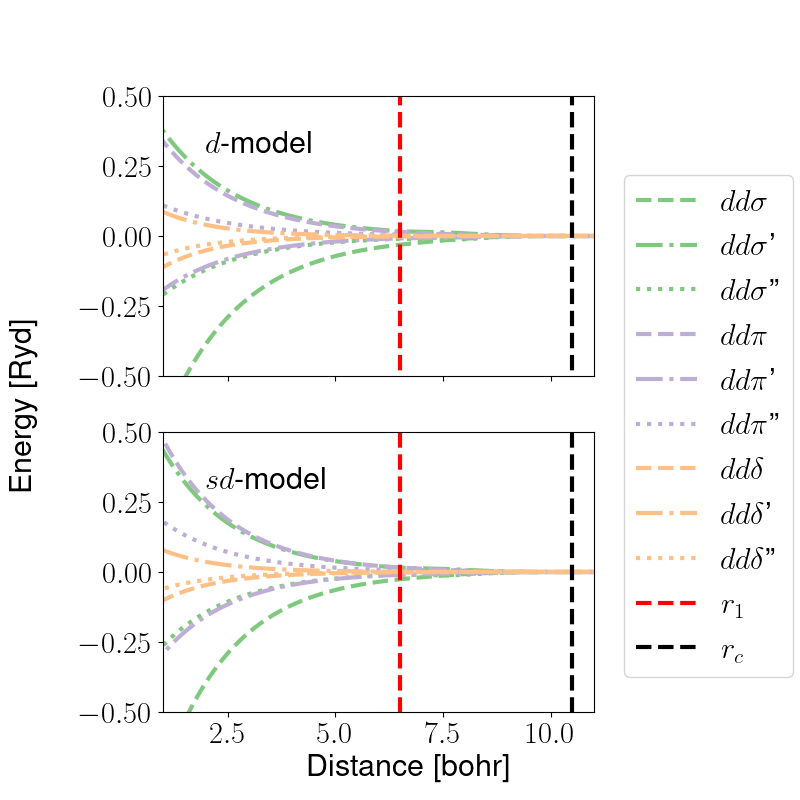
\includegraphics[width=\textwidth]{./images/d_sd_bond_integrals.png}
    \caption[Bond integrals of both $d$ and $sd$ titanium tight-binding models.] {Bond integrals of both $d$ and $sd$ titanium tight-binding models. First and second derivatives shown to demonstrate that there are no abberations when the bond integrals decay to zero between $r_1$ and $r_c$.} %square is table contents, curly is in the chapter
    \label{fig:d_sd_bond_integrals}
  \end{center}
\end{figure}



\begin{table}[htbp]
\label{tab:orgaec642b}
\centering
\begin{tabular}{lrlr}
Quantity & \(d\) model & \(sd\) model & Target\\
\hline
a\textsubscript{hcp} & 5.58523112 &  & 5.57678969\\
c/a & 1.58371266 &  & 1.58731122\\
a\textsubscript{omega} & 8.93475285 &  & 8.73254342\\
c\textsubscript{omega} & 5.38726911 &  & 5.32343103\\
a\textsubscript{4h} & 5.57584691 &  & 5.56325146\\
c\textsubscript{4h} & 18.09810672 &  & 17.75908031\\
a\textsubscript{6h} & 5.57365569 &  & 5.54639384\\
c\textsubscript{6h} & 27.18378460 &  & 26.77136353\\
a\textsubscript{bcc} & 6.20079768 &  & 6.17948863\\
a\textsubscript{fcc} & 7.87290654 &  & 7.88677000\\
DE(o,h) & 0.58764167 &  & -0.63343333\\
DE(4h,h) & 1.58019500 &  & 3.17160000\\
DE(6h,h) & 2.48264833 &  & 3.72005000\\
DE(b,h) & 5.35128500 &  & 7.63520000\\
DE(f,h) & 3.78088500 &  & 4.51880000\\
c\textsubscript{11} & 171.60928873 &  & 176.10000000\\
c\textsubscript{33} & 198.90063708 &  & 190.50000000\\
c\textsubscript{44} & 47.42549704 &  & 50.80000000\\
c\textsubscript{12} & 94.65941969 &  & 86.90000000\\
c\textsubscript{13} & 61.22624060 &  & 68.30000000\\
M\textsubscript{freq}\textsubscript{0} & 2.59341377 &  & 2.85858719\\
M\textsubscript{freq}\textsubscript{1} & 2.59341378 &  & 2.85858719\\
M\textsubscript{freq}\textsubscript{2} & 2.59341378 &  & 2.85858719\\
M\textsubscript{freq}\textsubscript{3} & 2.59341379 &  & 2.85858719\\
M\textsubscript{freq}\textsubscript{4} & 5.85272461 &  & 5.66706047\\
M\textsubscript{freq}\textsubscript{5} & 5.85272461 &  & 5.66706047\\
H\textsubscript{freq}\textsubscript{0} & 3.82320403 &  & 4.80643423\\
H\textsubscript{freq}\textsubscript{1} & 3.82320403 &  & 5.58010025\\
H\textsubscript{freq}\textsubscript{2} & 6.40288977 &  & 5.65316738\\
H\textsubscript{freq}\textsubscript{3} & 6.40288977 &  & 6.36651842\\
H\textsubscript{freq}\textsubscript{4} & 7.92857431 &  & 6.40050186\\
H\textsubscript{freq}\textsubscript{5} & 7.92857431 &  & 7.64082373\\
bandw.  G & 3.69394702 &  & 5.87085872\\
bandw.  K & 4.65178817 &  & 4.97424321\\
bandw.  M & 5.19329495 &  & 7.78109872\\
bandw.  L & 4.21232412 &  & 6.34433701\\
bandw.  H & 3.54700549 &  & 9.70902614\\
DOSerr\textsubscript{h} & 0.00000000 &  & 0.00000000\\
DOSerr\textsubscript{o} & 0.00000000 &  & 0.00000000\\
E\textsubscript{pris}\textsubscript{f} & 98.95340236 &  & 220.00000000\\
\end{tabular}
\end{table}

\section{sd fitting: Including hybridisation}
\label{sec:orge305c89}

We included s orbitals such that one could more readily model the
Ti\(^{4+}\) oxidation state of the Ti ion, which would give a more
physical representation of titanium ions in quantum electrochemistry
calculations.

\chapter{Methods}
\label{sec:org43387a2}

\section{Rugg}
\label{sec:org135f4e8}
Theoretical analysis showed 

Solute-dislocation interactions arise from two primary mechanisms:
elastic interactions mediated by the long-ranged strain fields
produced by a dislocation, and shorter-ranged interactions with the
dislocation core that are generally referred to as “chemical”
interactions (4, 6). The former are generally weak (on the scale of
\textasciitilde{}0.1 eV per solute atom); in fact, symmetry constraints have the
consequence that there should be no linear elastic interaction at
all between oxygen interstitials at octahedral sites and a straight
<a> screw dislocation in the hcp structure. Analysis is found in
the supplementary material. 


Short range interactions can change the restoring force of the
dislocation due to lattice slip. Which can by described by the
gamma surface energy. 

Two paths: 
\begin{itemize}
\item I  = octahedral site in perfect lattice
\item II = Newly formed octahedral site formed by slip of 0.5a

\item If oxygen on path of the slip plane (prismatic, I assume)
\begin{enumerate}
\item GSF energy is much higher than for pure ti
\item Original octahedral site gradually disappears and transforms
to a tetrahedral site with a lower interstitial volume, when
the magnitude of the slip is 0.5a.
\item Concurrently, a new octahedral site is formed on the basal
plane of the Ti structure.
\item Changing from the tetrahedral to the new octahedral site
reduces the energy by as much as 1.6 eV.
\item These results give a barrier for oxygen shuffle (hopping) from
path I to path II varies between 0.45-0.95eV, depending on
magnitude of slip displacement, which gives a large diffusion
barrier.
\item Large increase in energy coupled with the large diffusion
barrier means that the oxygen cannot move and thus there are
strengthening effects.
\item The volume changes can be correlated with changes in
interstitial volume upon dislocation slip.
\item The most pronounced volume changes occur on the prismatic slip
plane, where the core structure of the dislocation is spread.
\item Interaction energies are apparently quite weak (\textasciitilde{}60meV on neighbouring
prismatic planes to the dislocation spread) or a distance
larger than c/2 on the prismatic plane of the dislocation
spread.
\item With oxygen in the vicinity of the dislocation core there is
a strong repulsive interaction which causes the dislocation
to cross slip onto an adjacent prismatic plane.
\item If oxygen is on the basal plane (path II) then there is only
a small repulsive interaction (-50meV).
\end{enumerate}
\end{itemize}


So arguments summarised as follows:
\begin{enumerate}
\item As evidenced by oxygen being found on basal planes in lightly
deformed samples, due to the slip of a dislocation deforming the
octahedral site into one of a smaller interstitial volume,
oxygen will change site to an octahedral void on the basal plane
of the dislocation, where the oxygen will remain 'stuck'.
\item Cross-slip of the dislocation may occur onto another prismatic
plane. This will generate edge segments which connect the two
screw dislocations in each of their planes. These edge segments
can only move on the basal planes perpendicular to the prismatic
planes. Due to the high GSF energy, their mobility is limited.
\item The resolved shear stress to move these edge segments is zero if
one were to apply stress to cause the dislocation to move on the
prismatic plane. This effectively causes a pinning effect of the
oxygen near the dislocation core, providing a mechanism for
oxygen solute strengthening.
\end{enumerate}

\section{Chaari}
\label{sec:org7725474}

\begin{itemize}
\item Know that dislocation, in plane wave codes, seems to have a
ground state in the first order pyramidal plane and to move it
must change into a metastable state dissociated on the prismatic
plane to glide easily. This is the locking-unlocking mechanism of
Rodney.
\item Extend work of Rugg to see how oxygen can change the transitions
between core states which allow for glide.

\item Main results are
\begin{enumerate}
\item When the oxygen is placed in an octahedral site which is
destroyed upon dissociation of the dislocation into partials on either the
ground-state pyramidally spread core or the metastable
prismatic core, the core transforms to a compact
one, due to the strong repulsive effect of the oxygen. (This
site is the one between the partials.)
\item When the oxygen is away from the dislocation centre of the prismatically
spread configuration, the core is destabilised and it falls
into the ground-state prismatically spread configuration.
\item The narrowing of spreading (changing to compact core from
oxygen near the partials) can be evidenced by Yu, where
HAADF-STEM observations found that the dislocation core of
titanium was smaller with 0.1wt\% oxygen, where oxygen was
found in the core vicinity.
\item Yu \emph{et al} used a cell height of only one burger's vector, so
their interaction energies differ from those found by Chaari
(3b cell height). The interaction energies are much higher in
this work.
\item In the sites created by the stacking fault ribbon on
dissociation, the core configuration is stable.
\item The third case, where the stacking fault ribbon on the
pyramidal plane creates a new site by the pyramidal fault,
which correspond to octahedral sites in the twinned hcp
crystal For the pyramidal/mixed prismatic-pyramidal core
configurations, where this site is created, one finds that the
core remains/becomes close to the mixed prismatic-pyramidally
spread core.
\end{enumerate}
\end{itemize}

Conclusions

\begin{enumerate}
\item Lowest energy core configuration in Ti-O alloys is the
pyramidally spread core.
\item Predict that oxygen does not segregate to dislocations in these
alloys.
\item When a glissile prismatic core encounters an oxygen atom, the
core transforms to one that is pyramidally spread, to avoid the
obstacle.
\item This is evidenced by shorter glide distances on the prismatic
plane between pinning points in experiments.
\item Due to this cross-slip, jogs are formed, which agrees with
\emph{post-mortem} analysis showing that most screw dislocations have
jogs in the presence of oxygen. This explains high lattice
friction.
\item At higher temperatures, the bypass mechanism will be in
competition with oxygen migrating out of the repulsive region,
allowing the dislocation to remain in its glide plane.
\item A reconstruction of the pyramidal core induced by interaction
with oxygen allows us to understand why cross-slip in pyramidal
planes becomes more active with the addition of oxygen. And it
can glide in the pyramidal plane by nucleation of kink-pairs.
\end{enumerate}








\chapter{What did each method find}
\label{sec:org9822d6f}

\chapter{}
\label{sec:org933235b}

\chapter{Dislocation-carbon interactions in Fe-C}
\label{sec:orgb88bba5}
\label{chapter:dislocation_carbon_FeC}

\section{Introduction}
\label{sec:orgabbe8cc}

Martensitic steels are frequently used in bearings due to their resilience to service conditions,
being subject to high rotational speeds and contact pressures. However, under cyclic loading
exceeding a given contact stress, the microstructure of the steel can decay due to the accumulation
of plasticity. This signals the onset of rolling contact fatigue (RCF), which increases the risk of
failure from subsurface crack initiation. The microstructural decay corresponds to the observation
of Dark Etching Regions (DERs) as seen in optical microscopy, where the darkness of these regions is due
to the higher reactivity of DER phases to the etchant; exacerbated by
the roughness of the DER region \cite{skf2019}. See figure \ref{fuderpicture}.

\begin{figure}[htbp]
\centering
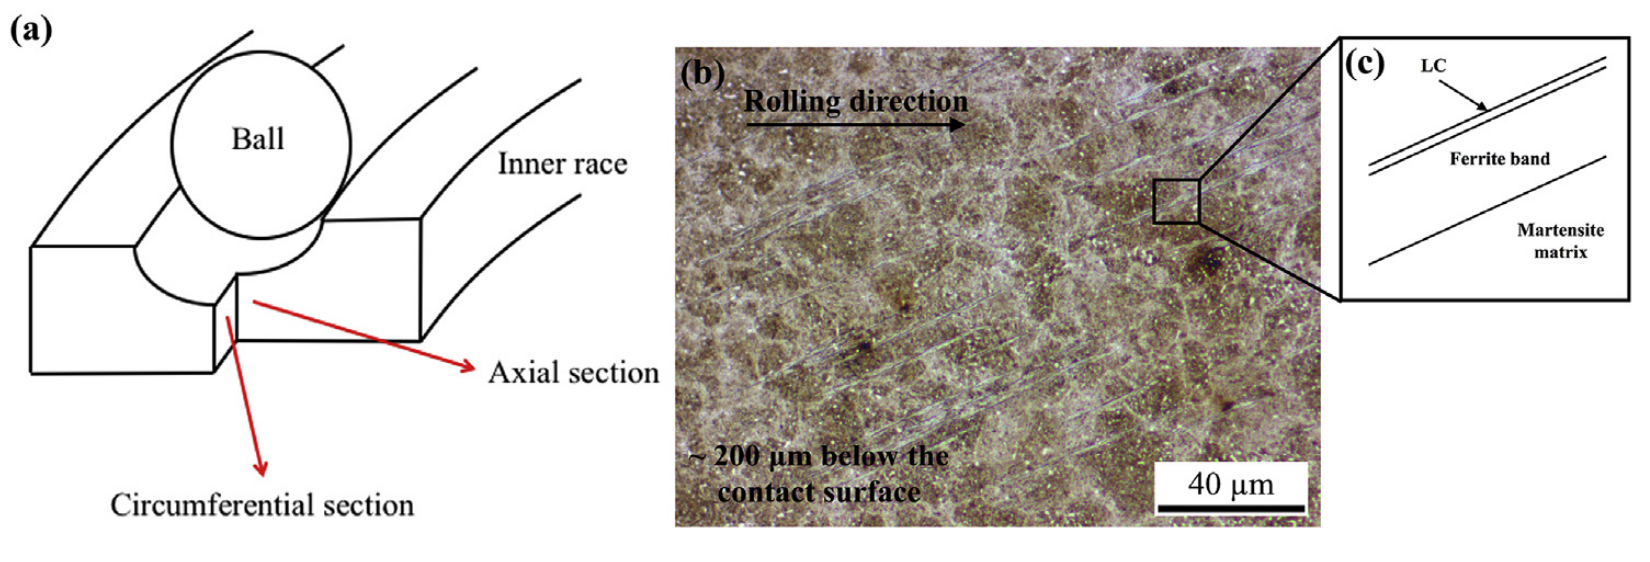
\includegraphics[width=.9\linewidth]{/home/tigany/Documents/docs/Management/Images/der_picture_fu.png}
\caption{Diagram of DER location within a bearing and its characteristics, taken from \cite{Fu2017}. (a) Axial and circumferential sections of a bearing inner ring. (b) Circumferential section of a bearing inner ring under optical microscope, where ferrite bands (white etching bands) are formed in the subsurface. (c) Diagram showing the structure of a WEB consisting of a ferrite band and a LC adjacent to it. One can see the DER region is composed of regions of ferrite interspersed in the parent martensite with lenticular carbides bordering the ferrite bands. \label{fuderpicture}}
\end{figure}


Decay of the martensitic microstructure is complex, with observation of many different
phenomena. Martensite transforms to ferrite microbands as a result of strain localization
\cite{Fu2017,il_micros_alter_rollin_contac_fatig,jonesil_metal_obser_ball_bearin_fatig_phenom,70_micros_microh_resid_stres_chang,Swahn1976,Voskamp1997,voskamp97_state_resid_stres_induc_by,polonsky95_white_etchin_band_format_rollin_bearin,vsmelova17_elect_micros_inves_micros_alter}. Residual
carbides, untouched at the start of DER formation, gradually dissolve within ferrite and
martensite \cite{70_micros_microh_resid_stres_chang,Swahn1976,Osterlund_1980}. Further RCF
progression leads to the formation of low and high angle ferrite features, White Etching Bands
(WEBs), composed of nanocrystalline \cite{Voskamp1997,Osterlund_1980,Mitamura_2007} and elongated
ferrite \cite{vsmelova17_elect_micros_inves_micros_alter}. Lenticular carbides precipitate at the
boundaries of these ferrite bands \cite{Swahn1976,Osterlund_1980}. Thickening of these carbides
occurs during DER development and is correlated with WEB growth
\cite{Fu2017,fu17_strain_induc_marten_decay_bearin,Warhadpande1_2013,Warhadpande2013}. Reductions in
dislocation density in nanocrystalline (heavily deformed) ferrite have been observed in the later
stages of DER formation \cite{skf2019,voskamp80_gradual_chang_resid_stres_micros}.



Carbon migration is thought to be the mechanism by which this degradation occurs, but it is not
definitively known how or where carbon migrates with the onset of DER formation. The key questions
are: where does excess carbon from the martensitic matrix find itself when the structure decays to
low solubility (0.02 wt\%) ferrite? and how is the carbon transported, given its low diffusivity in
martensite/DER phases
\cite{hashemi11_stren_hardn_statis_correl_api_x65_steel}?


Fu \emph{et al.} propose that carbon atoms inside the martensite would segregate to
pre-existing/residual carbides, increasing their size
\cite{fu17_strain_induc_marten_decay_bearin}. This theory was successfully applied to the
growth of lenticular carbides \cite{Fu2017}, however, problems arise with the application to
temper carbide growth: if carbides were to form in martensite, they should follow the
Bagaryatskii/Isaichev orientation relationship, but observations suggest a lack of any orientation
relationship \cite{Bhadeshia2018}. Temper carbides residing within DERs have irregular
shapes/diffuse boundaries, which are seemingly due to the incomplete \emph{dissolution} of \emph{temper}
carbides, which is at odds with the theory of Fu \emph{et al.}.

A plausible mechanism for carbon migration is that it is driven by dislocation glide, which is as
follows
\cite{Fu2017,Swahn1976,voskamp97_state_resid_stres_induc_by,fu17_strain_induc_marten_decay_bearin,Warhadpande1_2013,Warhadpande2013}. Due
to the high dislocation density exhibited in martensite, carbon segregates to dislocations in
Cottrell atmospheres, causing pinning. Strain generated by cyclic stresses allow dislocations to
escape their carbon rich environment. The free dislocations re-attract carbon, allowing the
Cottrell atmospheres to reform, subsequently re-pinning the dislocations, creating a net carbon
flux.  This mechanism allows for the movement of carbon during the martensite-ferrite transition,
while also explaining how excess carbon can move from the ferrite phases to lenticular carbides at
the boundaries, describing the process behind both WEB growth and carbide thickening. Moreover, it
explains the dissolution of residual carbides, both in ferrite WEBs and martensite, due to
dislocation rearrangement and pile ups at the carbide interface drawing carbon atoms out, due to a
more favourable binding to dislocations. However, as to how this process occurs on the atomistic
scale, or if it is indeed feasible, is unknown.



Experimentally probing dislocation-assisted carbon migration has proven difficult and inconclusive. Work needs to be done
to understand dislocation-carbon interactions; more specifically: how dislocations move carbon
within the temperature and stress regimes experienced during operation; where carbon is
transported to and what the resultant dislocation networks are.


To shed light on this mechanism, a multi-scale modelling approach can be
used. Atomistics can provide information of the 2d Peierls energy landscape which dislocations are
subject to in iron; and how this landscape is modified by the binding of carbon to
dislocations. This data can be used in a line tension model of a dislocation to determine the
kink-pair formation energies of dislocations as a function of carbon content and stress. Finally,
one can use a kinetic Monte Carlo (kMC) model of dislocation glide by thermally activated
kink-pair nucleation, in an environment of carbon. From this last stage of coarse-graining, one
can determine in which regimes of temperature, stress and carbon concentration,
dislocation-assisted carbon migration becomes a feasible mechanism behind DER formation, with
predictions of dislocation velocity, dislocation configurations and where carbon moves with
dislocation glide.

In this report, we will focus on the atomistic portion of this project,
directed at understanding dislocation-carbon interactions at the atomistic scale in ferrite (bcc
iron).
With further knowledge of the fundamental mechanism behind DER formation, we can hope to suppress
dislocation motion in the martensitic matrix, mitigating failure by RCF.



\section{Computational Method}
\label{sec:orgf447060}


We use the tight-binding model of Paxton and Elsässer \cite{Paxton2013}, which has been shown to
describe the binding energies of carbon complexes in bcc iron, in good agreement with DFT
calculations. This model reproduces the two screw dislocation core structures---the easy and hard
\(1/2\langle 111 \rangle\) cores---exhibited in bcc iron. Study of both is crucial to understanding
solute-dislocation interactions. The easy core is the ground state in pure iron, but solutes, such
as hydrogen and carbon, have been shown to reconstruct this core into the hard core
configuration \cite{Ventelon2015,itakura13_effec_hydrog_atoms_screw_disloc}. Computationally cheaper
models, which do not incorporate quantum mechanics, such as the EAM, cannot reproduce these
behaviours.


\subsection{Peierls Potential}
\label{sec:orgd9b90dc}

To determine the Peierls potential of the \(1/2\langle 111 \rangle\) screw dislocation, we followed the
procedure detailed in Itakura \cite{Itakura2012}. Quadrupolar arrays of dislocations were
constructed by placing dislocations of antiparallel \(1/2\langle 111\rangle\) Burgers vectors in an "S"
arrangement \cite{Clouet2012}, with initial displacements determined by anisotropic elasticity
solutions. See figure \ref{fig:dislocationschematics}, left. A quadrupolar arrangement minimises
the stress each dislocation experiences in the simulation. These displacements were modified to
be periodic, thereby removing artificial stacking faults which would appear between periodic
images after introduction of the dislocation dipole. This was achieved by the subtraction of a
linear error term from the superposition of displacement fields arising from the dislocations in
the simulation cell and its periodic images \cite{vasilybulatov2006}. To accommodate for the
internal stress upon introduction of a dislocation dipole into the simulation cell, an elastic
strain was applied to the cell, resulting in an additional tilt component to cell vectors
\cite{Clouet2012,vasilybulatov2006,Clouet2009}. Simulation cells were constructed with different initial core
positions, which were sampled from the triangular region "EHS" (easy, hard and split) core
positions, as detailed in figure \ref{sampledpositions}. To fix the dislocation positions during
relaxation, the three atoms surrounding the easy core, for each dislocation, were fixed in \(Z\)
coordinate during relaxation, where \(Z\) is a \(\langle 111 \rangle\) direction, along the dislocation line. The
k-point sampling mesh for each of these cells was 5x5x30.


        \begin{figure}
    \begin{tabular}{cc}
	     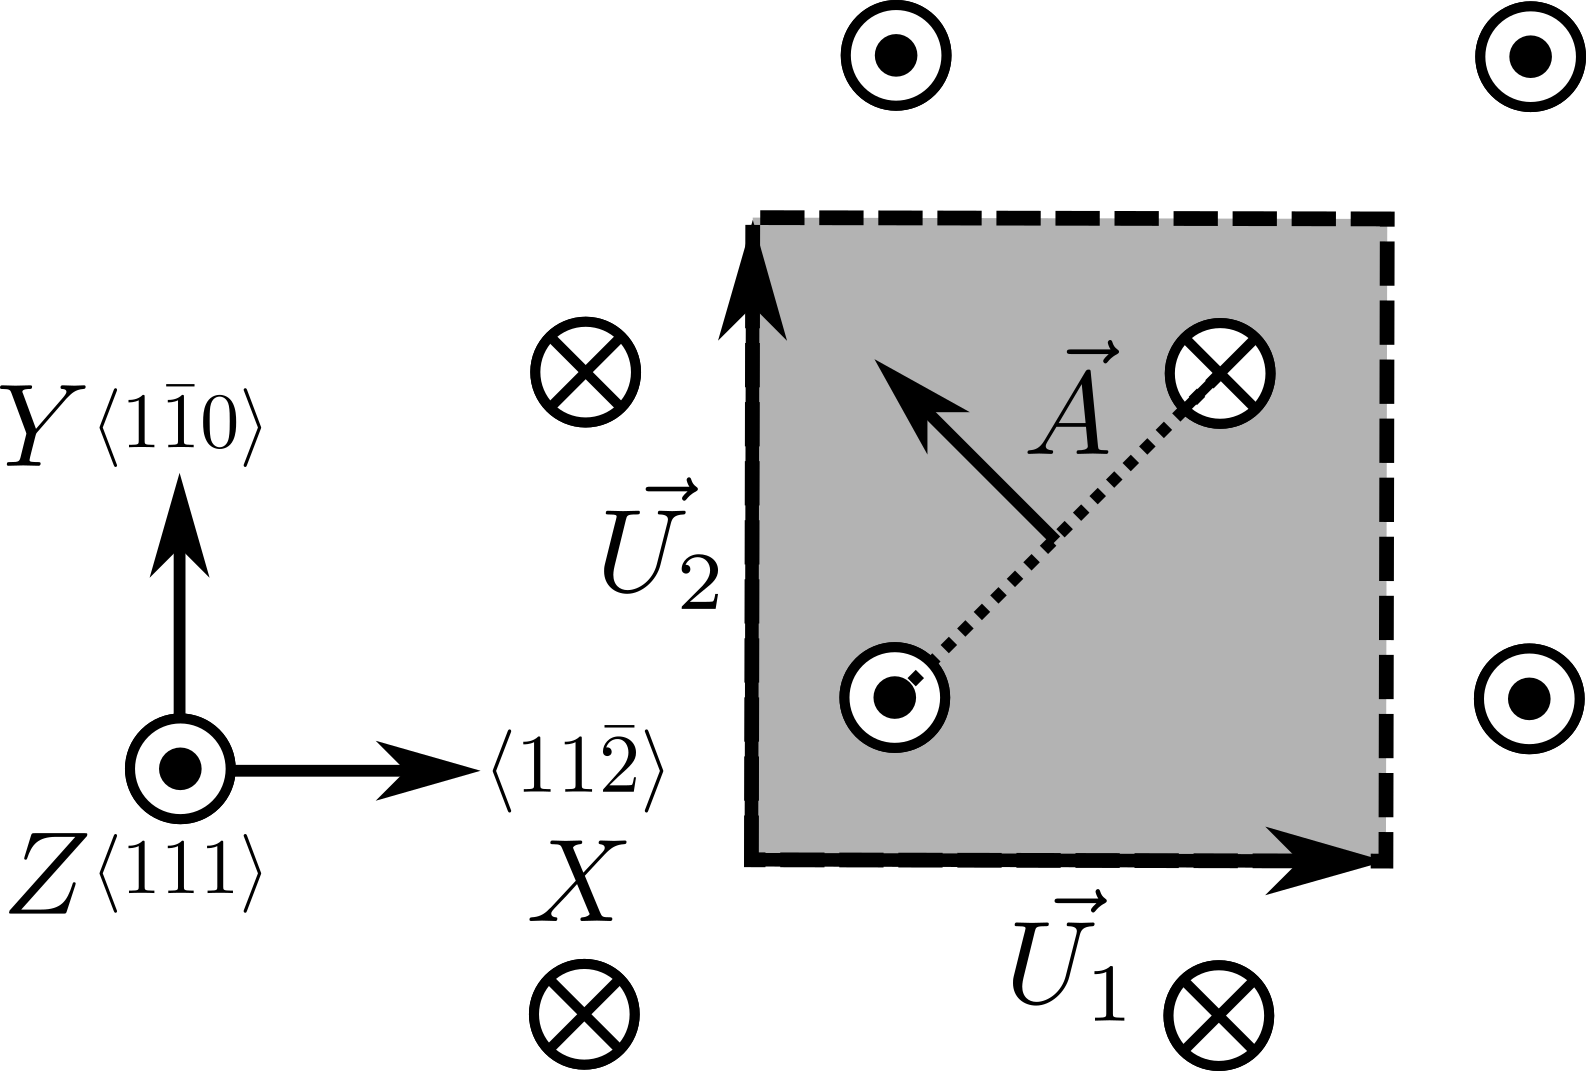
\includegraphics[width=0.5\textwidth]{Images/s_arrangement_quadrupole.png} &
             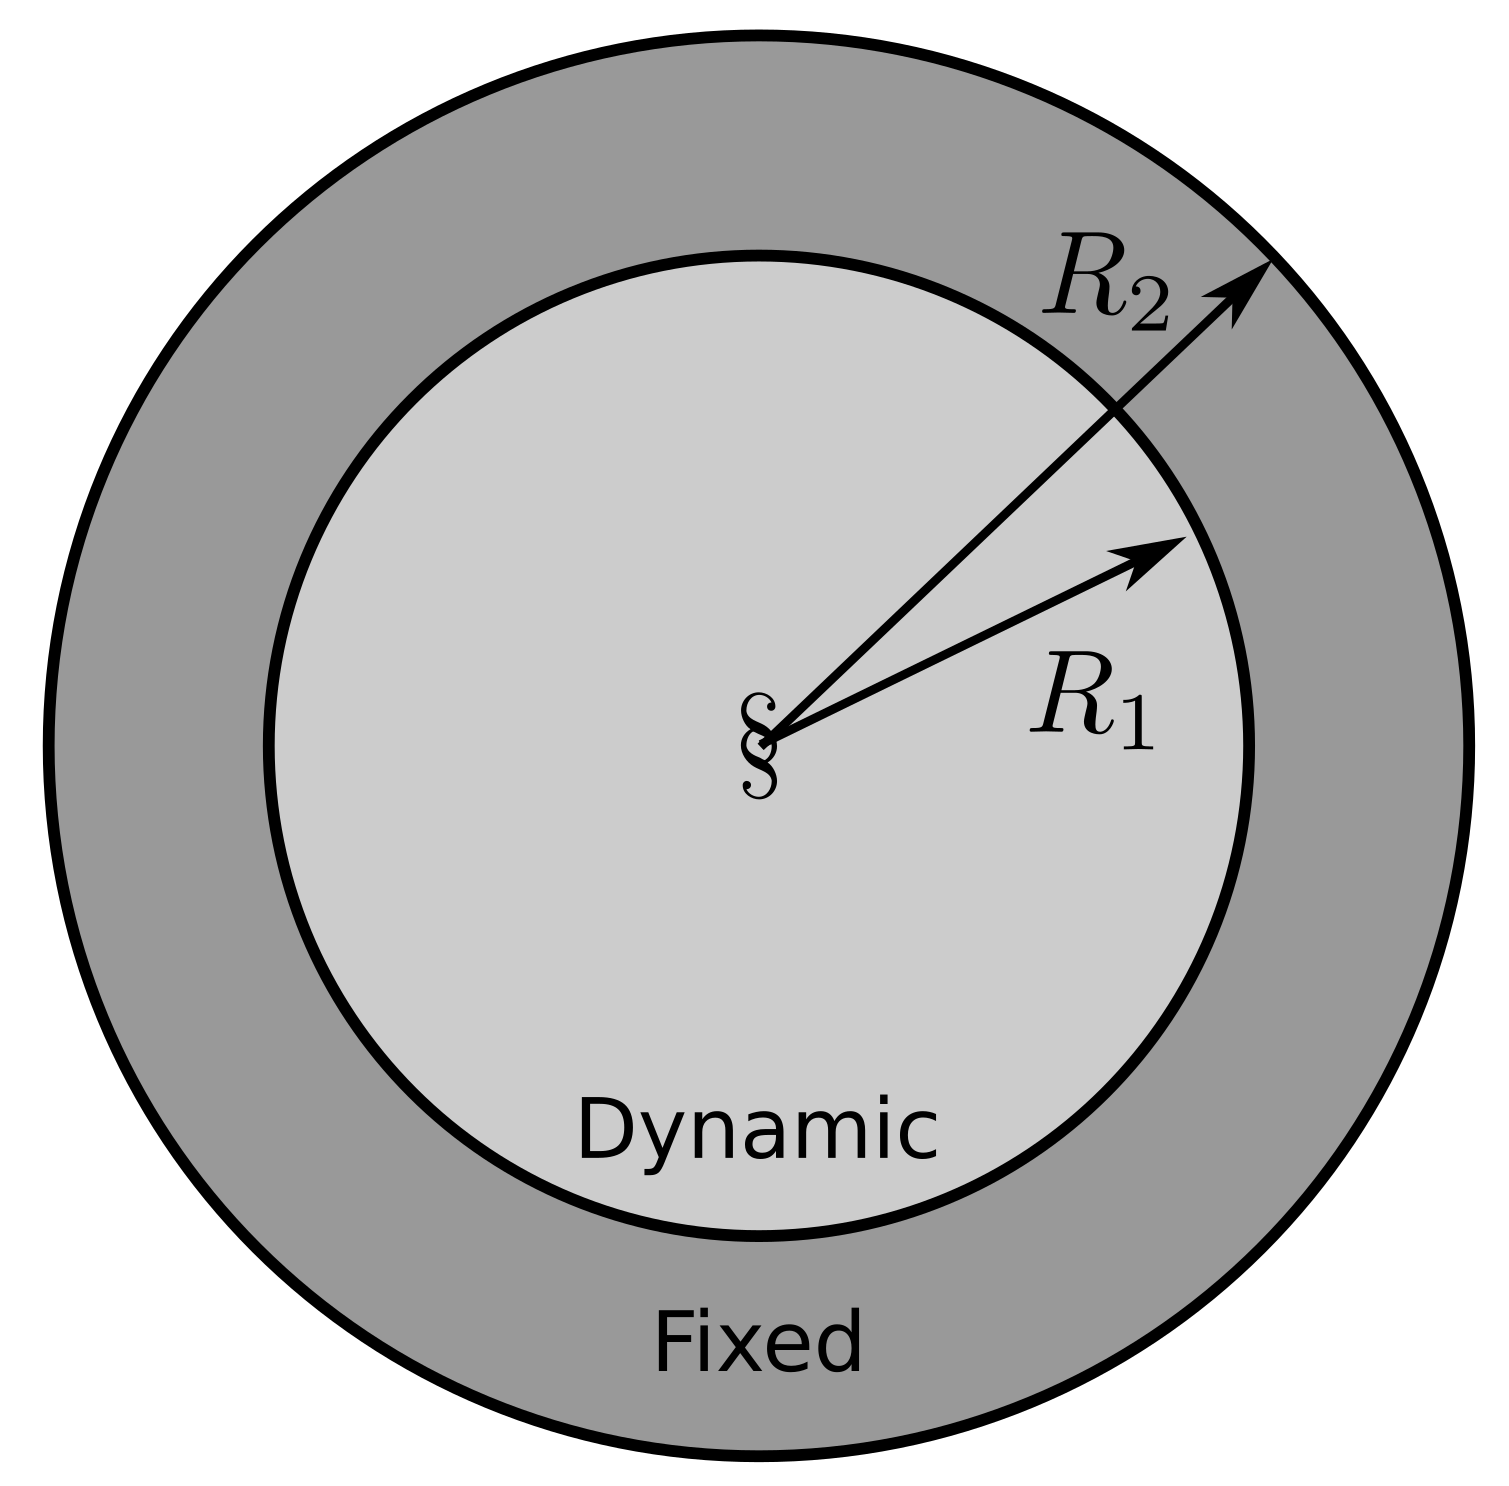
\includegraphics[width=0.45\textwidth]{Images/cluster_method_schematic.png}  \\
    \end{tabular}
\caption{Schematics of dislocation simulation methods. Left: quadrupolar arrangement of dislocations in a simulation cell (grey square). This arrangement  minimises the stress experienced by each dislocation in a periodic simulation. Cell vectors $\vec{U}_1$ and $\vec{U}_2$ are shown; $\vec{A}$ defines the cut plane between the dipoles. The dislocation positions, and their corresponding burger's vector direction, are denoted by the symbols $\otimes$ and $\odot$, which are antiparallel to each other. Tilt components added to cell vectors to accomodate for the plastic strain are not shown. Right: cluster method, where atoms are displaced according the displacement field from the screw dislocation at the centre of the cluster, denoted by "\S". Atoms in the annulus $R_2 - R_1$ are fixed in position to the anisotropic elasticity solutions. Within $R_1$, all atoms can relax. Periodicity is only imposed in the $Z$ direction.}
	\label{fig:dislocationschematics}
    \end{figure}



        \begin{figure}
    \begin{tabular}{cc}
	     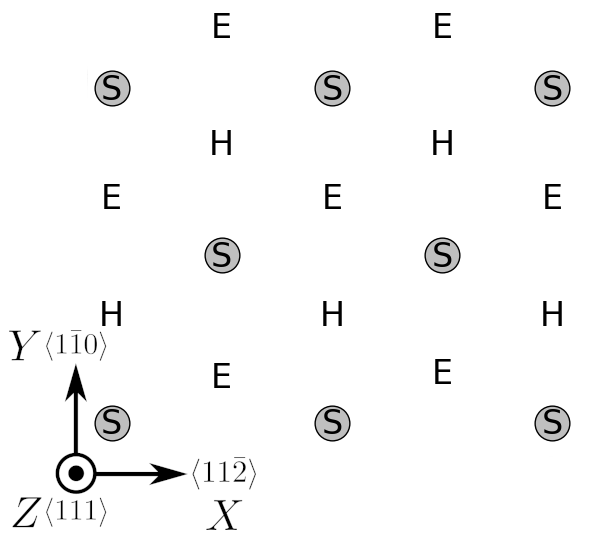
\includegraphics[width=0.5\textwidth]{Images/hardeasycoreatomdiagram_coordnew.png} &
             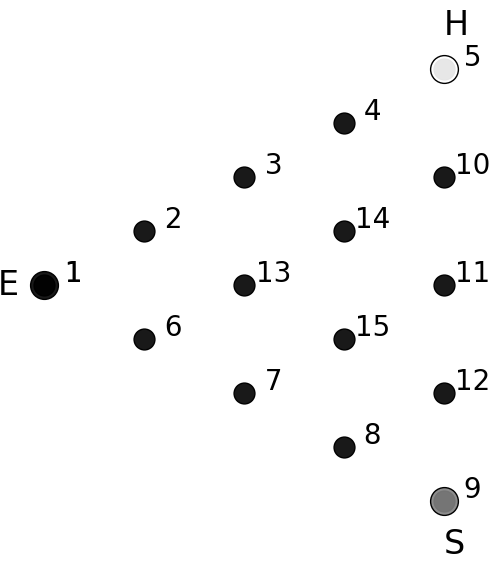
\includegraphics[width=0.45\textwidth]{Images/peierls_potential_positions_tbe.png}  \\
    \end{tabular}
\caption{Diagrams of dislocation core positions. "E", "H" and "S" correspond to the easy, hard and split core positions respectively. Left: core positions as seen along the $Z=\langle 111 \rangle$ direction, along the dislocation line. Atomic positions are shown as grey circles. Right: positions sampled within the triangle EHS used to determine the Peierls potential.  \label{sampledpositions}}
	\label{fig:peierlspot}
    \end{figure}


The interaction energy between the dislocation dipole and periodic images was defined differently
to Itakura \cite{Itakura2012}. We followed the prescription of Bulatov and Cai \cite{vasilybulatov2006} to
find a regularised interaction energy, which is independent of truncation limit, in contrast to
the formulas quoted in Itakura's papers. Details can be found in section \ref{sec:Ainteractionenergy}.




The Peierls potential \(\Delta E_{\text{P}}^i\), for an isolated dislocation at the \(i^{\text{th}}\) core
position, can be calculated from
\begin{equation}
 \Delta E_{\text{P}}^i = \Delta E_{\text{tbe}}^{i} - \Delta E_{\text{INT}}^{i} ,\label{eq:peierlspot}
 \end{equation}
where \(\Delta\) refers to quantities, per dislocation, relative to the relaxed easy core configuration
(labelled as E/1, as in figure \ref{sampledpositions}). \emph{e.g} \(\Delta E_{\text{tbe}}^{i} = \frac{1}{2} (
    E_{\text{tbe}}^{i} - E_{\text{tbe}}^{\text{E}} )\) is the difference in energy, per dislocation, between
a relaxed cell which has the two dislocation cores placed at position \(i\), \(E_{\text{tbe}}^{i}\), and a relaxed
cell which has the two cores placed in easy core positions \(E_{\text{tbe}}^{\text{E}}\), divided by the number of
dislocations in each of the simulation cells. Dislocation-dislocation interaction
energies are included in this term, due to dislocations in the simulation cell---and
periodic images---interacting with each other, as can be readily seen in figure
\ref{fig:dislocationschematics}. To model the energy landscape of an isolated dislocation, these
interaction energies must be subracted, which is achieved by the correction term \(\Delta E_{\text{INT}}^{i}
    = \frac{1}{2} ( E_{\text{INT}}^{i} - E_{\text{INT}}^{\text{E}} )\).

\subsection{Preliminary calculations}
\label{sec:orgeb0168d}

To determine the binding energy of carbon to dislocations, we used the cluster method, as shown
in figure \ref{fig:dislocationschematics}, right. Simulation
cells consisted of a cylindrical cluster of atoms, with a single dislocation introduced into the
centre using displacements from anisotropic elasticity solutions. Each of the clusters were
centred on the easy or hard core positions. The cluster of atoms was split into two regions: a
central region of dynamic atoms with radius \(R_1\), and an annulus of atoms, between \(R_1\) and \(R_2\),
which were fixed in position to the displacements from anisotropic elasticity.


To confirm the anisotropic elasticity solutions were correct, we compared the
displacements against the analytic solutions to the straight screw dislocation, as given in Hirth
and Lothe \cite{Anderson2017}. Furthermore, energy scaling relations were verified. We
inserted dislocations into cells of varying radii: \(R_1 = x\sqrt{2}a_{\text{bcc}}\), and \(R_2 =
    (x+1)\sqrt{2}a_{\text{bcc}}\), where \(x \in \{2\dots5\}\). The excess energy
was defined as the energy difference of a cell with a dislocation inserted, \(E_{\text{d}}\), with
respect to a perfect cell reference energy of the same geometry,

\begin{equation}
 E_{\text{excess}} =   E_{\text{core}} + E_{\text{elastic}} = E_{\text{d}} - E_{\text{perfect}}   ,\label{eq:excessenergy}
 \end{equation}
where
\(E_{\text{elastic}} = ( \mu b^2 / 4\pi )\ln (R/ r_c)\), with \(R = R_2\) and \(r_c = b\).

Initially, large cells of \(R_1 = 6\sqrt{2}a_{\text{bcc}}\), and \(R_2 =
    7\sqrt{2}a_{\text{bcc}}\) with depth of single burger's vector, were relaxed
for both the easy and hard cores, which consisted of 522 and 540 atoms
respectively. The three atoms surrounding the core were constrained to only
relax in \(X-Y\) plane, to fix the dislocation upon relaxation.
The k-point sampling mesh for each of these cells was 1x1x24.

From the relaxed cells, a smaller region of 174 atoms, with \(R_1 = 3\sqrt{2}a_{\text{bcc}}\), and \(R_2
    = 4\sqrt{2}a_{\text{bcc}}\), was cut from the dynamic regions. This smaller cell was extended to a
thickness of 3\(b\) in the \(Z\) direction. Carbon interstitials were inserted into octahedral sites
near the dislocation core, in the middle layer. Exploiting reflection and rotational symmetry,
only 10 interstitial sites needed to be used to obtain the binding energies of carbon \(\sim2\) b from
the core, denoted by iH\(j\) and iE\(j\), where \(j \in \{1\dots10\}\). The final binding sites are denoted
by H\(k\) and E\(j\), where \(k \in \{1\dots7\}\). The three atoms surrounding the core in the first and
third layers were again constrained to relax only in the \(X\) and \(Y\) directions. No such
constraints were imposed on the middle layer.

Interestingly, if one to pre-emptively include the distortion
carbon into the cell, by superposing the displacement field
generated from carbon in an otherwise perfect cell of 3b
length---one does not find the true ground state structures, as
predicted by dipole calculations which allow all degrees of freedom
to be relaxed.

\subsection{Fe-C binding energies}
\label{sec:org06864d3}
We calculated the carbon-dislocation binding energies as in Itakura
 \cite{itakura13_effec_hydrog_atoms_screw_disloc}.

The binding energy is given by
\begin{equation}
E_b = -( E_{\text{d+C}} + E_{\text{perfect}}- E_{\text{d}} - E_{\text{C ref.} } ),
\end{equation}

where \(E_{\text{d+C}}\) is the total energy of a relaxed cluster with a
carbon interstitial and a dislocation, \(E_{\text{d}}\) is the total
energy of a relaxed cluster with a dislocation and \(E_{\text{C
     ref.}}\) is the total energy of a relaxed perfect cluster with a single carbon in
an octahedral site. A positive binding energy indicates favourable binding.

The zero-point energy (ZPE) is calculated as in Itakura. Details can be found in \ref{sec:zeropointenergy}.
The ZPE corrected binding energy is given by
\[ E^{\text{Z}}_{b} = E_b + \Delta E_z,  \]
where \(\Delta E_z = E_z - E_{z}^{\text{C ref.}}\) and \(E_{z}^{\text{C ref.}} = 202.5 \text{meV}\) is the zero-point energy of carbon
situated in an octahedral site in a perfect cluster of the same size.

Calculations were also
\subsection{Carbon concentration on dislocation line}
\label{sec:org5b4d1d0}
\label{sec:carbon_concentration}

Using the Fe-C binding energies, one can predict the equilibrium carbon
concentration of a carbon binding site \(c_d\), using a thermodynamical mean-field model \cite{Treglia1999,Ventelon2015,mclean1957grain}, under the
assumption that carbon atoms around the core are sufficiently spaced such
that intersite interaction energies are negligible.

The concentration is given by,
\begin{equation}
\frac{ c_d^{i} }{1 -  c_d^{i} } = \frac{ c_{\text{bulk}} }{1 - c_{\text{bulk}} } \text{exp} \Big(
\frac{-E_{\text{seg}}^i(c_d)}{k_{\text{B}}T}  \Big),    \label{eq:cd}
\end{equation}
where \(i\) denotes the \(i^{\text{th}}\) carbon binding site.
\(E_{\text{seg}}^i\) is the mean segregation energy defined as

\[ E_{\text{seg}}^i(c_d) = -E_{\text{b}}^{i} + 2c_d
     V_{\text{CC}},\]

where \(E_{\text{b}}^{i}\), is the corresponding dislocation-solute binding
energy (in the convention of attraction denoting a positive binding
energy). \(c_d^{i}\) is the average concentration of the \(i^{\text{th}}\)
carbon site bound to dislocations. \(c_{\text{bulk}}\) is the carbon
concentration in the bulk, with \(c_{\text{nom}}\) the nominal carbon
concentration per Fe atom. \(V_{\text{CC}} = 0.30 \text{eV}\) is the carbon-carbon
first-neighbour repulsion term, which is calculated as in Ventelon
\cite{Ventelon2015}. This repulsion term was calculated from carbon in the H1
prismatic site. It was assumed that this repulsion term is the same for
carbon in the E2 site.


In a given volume \(V\), the number of carbon sites along the dislocation
cores is given by \(N_d = \rho V/b\), with \(\rho\) the dislocation density, and
the number of octahedral sites is \(N_{\text{oct}} = 6V/a_{\text{bcc}}\). This
imposes constraints on the carbon concentrations: \(N_{\text{oct}}
     c_{\text{bulk}} + N_d c_d = N_{\text{oct}} c_{\text{nom}}/3\), where the
factor of 3 is because there are three octahedral sites per Fe atom in the
bcc lattice. Using this relation, equation \eqref{eq:cd} can be solved
self-consistently to give the carbon concentration around the core, as a
function of nominal carbon concentration and temperature. The nominal carbon
concentration was taken to be the maximum solubility of ferrite in the DER
region, 0.02 wt\% \(\approx 1000\) appm
\cite{hashemi11_stren_hardn_statis_correl_api_x65_steel}. Calculations of 10
and 500 appm were also performed. The dislocation density was varied between
\(1\times10^{12}\), \(1\times10^{14}\) and \(5\times10^{15}\), to see the effects
of low densities up to the upper bound of dislocation densities
\(\sim5\times10^{15}\) found in Fe-0.61wt\%C martensite
\cite{morito03_disloc_densit_within_lath_marten}.


Further discussion on carbon concentration formulations is given in section
\ref{sec:concentration_statistics_discussion}.

\subsection{Line Tension Model}
\label{sec:org8f75a83}
\label{sec:ltmodelintro}

The kink-pair formation enthalpy is defined as the minimum energy necessary to to
create a kink-pair from a dislocation in a Peierls valley. One can find this by
sampling the energy landscape seen by a dislocation line which moves one peierls
valley to the next, from which the minimum enthalpy path can be sought. The difference
between the maximum enthalpy image, corresponding to a dislocation configuration in a
transition state, and enthalpy of the initial state, is the kink-pair
formation enthalpy. One can efficiently determine the minimum enthalpy path using the
String/Nudged Elastic Band (NEB) algorithms. In these methods, a set of images, which
interpolate between the initial and final states, are relaxed along the energy
landscape.


From atomistic calculations of the Peierls potential and carbon-dislocation binding energies, one
can construct a line tension model of a dislocation from which we can obtain the kink-pair
formation energies as a function of stress and carbon content
\cite{Anderson2017,Itakura2012,itakura13_effec_hydrog_atoms_screw_disloc}. This model views the
dislocation as an elastic chain which moves in the Peierls potential \(\Delta
    E_{\text{P}}\). Models of this type---consisting of a one-dimensional chain of particles with
spring force interactions between nearest-neighbours, in a substrate potential---are also called
Frenkel-Kontorova models, and have been crucial in some of the first investigations into
kink-pair formation, among other non-linear processes \cite{Braun1998,Kontorova1938,Frenkel1939,Rodney2009}.

The dislocation is modelled as a discretised line, with layer labels \(j\). The energy of the
dislocation line is given by:

\[ H_{\text{LT}}(\sigma) = \frac{K}{2} \sum_j (\vec{P}_j - \vec{P}_{j+1} )^2  + \sum_j \Delta E_{\text{P}}  (\vec{P}_j) +
    (\sigma \cdot \vec{b}) \times \vec{l} \cdot \vec{P}_j  - \sum_{j,k} E_{\text{C}} (|\vec{P}_j-\vec{P}_k^{\text{C}}|), \label{eq:line-tension}\]

where \(K\) is a constant calculated from atomistics, \(\Delta E_{\text{P}}\) is the
Peierls potential, \(\sigma\) is the stress applied and \(\vec{b}\) is the burger's vector,
with the dislocation line sense given by \(\vec{l}\). \(\vec{P_{j}}\) corresponds to the
dislocation core position in a given layer. \(E_{\text{C}}
    (|\vec{P}_j-\vec{P}_k^{\text{C}}|)\) is the binding energy of a particular carbon \(k\),
at position \(\vec{P}_k^{\text{C}}\), to a dislocation core positioned at
\(\vec{P}_j\). The kink-pair formation enthalpy can then be found using the string method
to relax images which interpolate between the initial and final states (straight
dislocations in adjacent peierls valleys), to find the height of the transition-state
barrier. A \texttt{julia} implementation of the string algorithm, accelerated by use of an ODE
solver, was used to relax the images \cite{Makri2019}. The implementation was validated
on the dataset of Itakura \cite{Itakura2012}.



\begin{enumerate}
\item Line-tension model in carbon environment
\label{sec:org2d1054d}

Dislocations form Cotrell atmospheres of carbon, which influence their
motion. Analysis of the dynamics of a dislocation moving from one Peierls
valley to the next, in an environment of carbon in equilibrium with the
bulk, can provide estimates of: the mean energy barrier experienced by a
straight dislocation segment upon glide, and the mean kink-pair formation
enthalpy, both as functions of nominal carbon concentration. Results of the latter
can be used as inputs to a self-consistent kinetic Monte-Carlo
(SCkMC) model of dislocation glide, which has been shown to predict
dislocation structures in hydrogen-charged iron \cite{Gong2020}. The kink-pair
formation enthalpy calculations in this paper study were performed in
the limit of slow dislocation glide, allowing carbon to equilibrate between
sites, however more accurate results may be possible by accounting for
dislocation velocity in a self-consistent manner.


The binding sites of carbon around the easy and hard core dislocation
positions were found from atomistic simulations, detailed in section
\ref{sec:fec_binding}. Movement of a dislocation between peierls valleys
generates intermediate core positions which lie between the easy and hard
cores. Carbon trap sites are not well-defined for these intermediate
dislocation positions. To circumvent this, trap site positions were smoothly mapped between
the easy and hard core positions by use of the dislocation core coordinate
\(P_x\). Further information on the mapping of sites can be found in appendix
\label{sec:smoothsitemapping}.


The carbon concentration on the dislocation line was calculated by the
self-consistent thermodynamical mean-field model, detailed in
\ref{sec:carbon_concentration}. The concentration was fixed to the value
obtained using the H1 binding energy, \(c_{\text{total}} = c_d^{\text{H}1}\),
imposing the assumption that the dislocation neither rejects or absorbs
carbon, despite changes in the carbon environment upon core
movement. Thus carbon concentration on the dislocation line remained in
equilibrium with the bulk during the simulations.

The equilibrium concentration of carbon in a trap site \(i\),
\(c_{i}^{\text{e}}\) was initially determined by use of
Maxwell-Boltzmann statistics \cite{Anderson2017}, as done by Cottrell and
Bilby \cite{Cottrell1949}, and Gong \cite{Gong2020},

\[  c_{i}^{\text{e}}(x) = c_d^{\text{H}1} \frac{ e^{-E_i(x) /
     k_{\text{b}} T } }{\sum_j e^{-E_j(x) / k_{\text{b}}T} }.  \label{eq:maxwellboltzmann_conc}\]

These concentrations modify the interaction energy of a given site
multiplicatively, such that the total interaction energy of a dislocation in
an environment of solutes is given by

\[ E_{\text{INT}}^{\text{e}} = \sum_j c_j^{\text{e}} E_j(x).\]


Kink-pair formation enthalpies were obtained using the string method, as
detailed in section \ref{sec:ltmodelintro}.


\item Extension to more Fermi-Dirac statistics
\label{sec:orgf4a60c0}
\label{sec:concentration_statistics_discussion}

Cottrell and Bilby's assumption of Maxwell-Boltzmann statistics, as seen in
equation \eqref{eq:maxwellboltzmann_conc}, is valid for small
dislocation-solute binding energies, which are generally found for solutes far from the
dislocation \cite{Veiga2013}. However, close to the dislocation core, we
expect a strong binding of carbon to dislocations, as such, Maxwell-Bolzmann
statistics fails to be a good description of carbon occupancies: one finds
unphysically large occupancies, due to carbon being able to occupy the same
site \cite{Nematollahi2016}.

For a more realisitic description of carbon occupancies, one must account
for the limited number of carbon sites close to the dislocation core, which
are either occupied or not. This problem, of distributing indistinguishable
particles (neglecting inter-/intra-site interactions) between sites which
can only be singly-occupied, is reminiscent of Fermi-Dirac statistics, which
was applied by Nematollahi \cite{Nematollahi2016} to treat carbon occupancies
around an easy core up to a cut off of 0.04---a result obtained by the EAM
calculations of Veiga \cite{Veiga2011}. This distribution was assumed to be
true, however, it neglected the effect of assumptions which were not
explicitly taken into account. Louat \cite{Louat1956} provided a more rigorous
derivation for the concentration of solutes close to the dislocation core,
which has been used by many in recent years
\cite{Ventelon2015,Treglia1999,mclean1957grain,Veiga2013,Luthi2019}. In this
formulation, it is assumed that the area around the dislocation is divided
into a number of sub-regions (an effective lattice) where only one solute
atom can occupy each position, and there are no inter-line or inter-site
interactions. One only accounts for the configurational entropy of the
effective lattice; electronic, vibrational and magnetic entropic
contributions are not taken into account \cite{Ventelon2015}. This treatment
of configurational entropy becomes inaccurate for low binding energies, as
noted the case of hydrogen/hydrogen-vacancy complexes in Fe
\cite{Davidson2020}: with low enough binding energies, the species is able to
move in a smooth and continuous potential, resulting in a larger
configurational phase space available than just the sampled binding sites
taken into. We expect due to the large binding energy of carbon to
dislocations, relative to hydrogen, for a range of distances, the
configurational entropy would not be significantly enhanced compared to the lattice model.
\end{enumerate}


\section{Results}
\label{sec:orgc951007}

\subsection{Peierls Potential}
\label{sec:org77730ee}

        \begin{figure}
\centering
    \begin{tabular}{c}
	     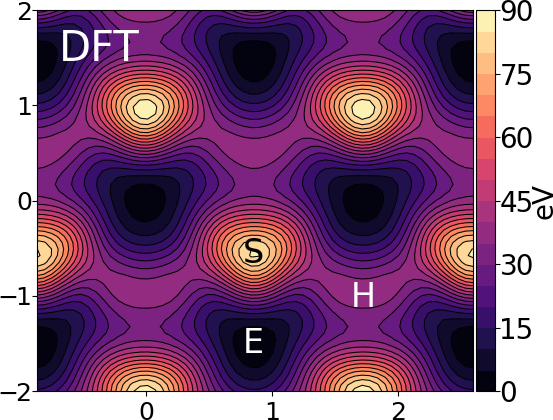
\includegraphics[width=0.5\textwidth]{Images/peierls_potential_dft_labelled_zeal.png} \\
             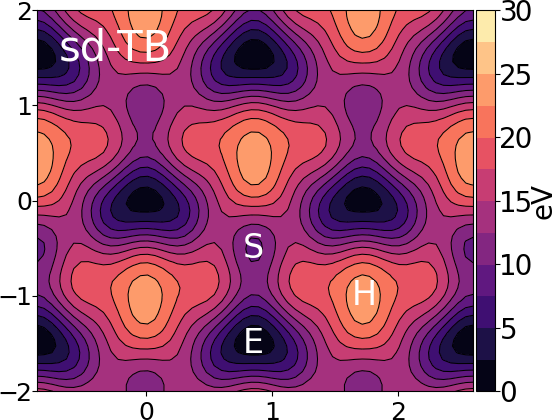
\includegraphics[width=0.5\textwidth]{Images/peierls_potential_sdTB_labelled_zeal.png}  \\
             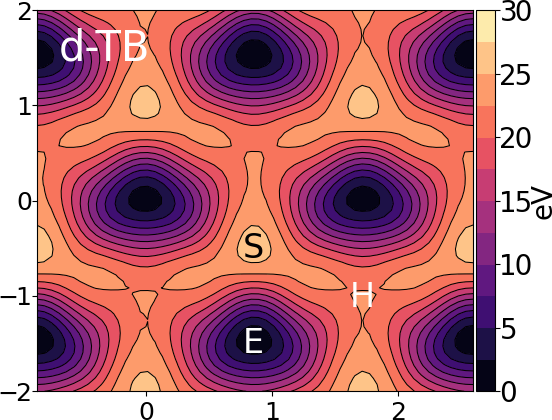
\includegraphics[width=0.5\textwidth]{Images/peierls_potential_dTB_labelled_zeal.png}  \\
    \end{tabular}
\caption{Comparison of 2d Peierls potentials of the $1/2\langle 111\rangle$ screw dislocation between DFT \cite{Itakura2012} (top) and tight-binding ($sd$ non-orthogonal middle, canonical d, bottom). $x-y$ axes in units of $d=a\sqrt{2} / 3$.Energy scale is in meV. "E", "H" and "S" correspond to easy, hard and split core positions respectively, with the latter also corresponding to atomic positions. The relative energies between the different core positions is smaller in tight-binding compared to DFT. The split core as seen in tight-binding is reminiscent of EAM potentials, where the split core energy is lower than that of the hard core. The discrepancy is probably due to an insufficient repulsion at close range within the tight-binding model.}
	\label{fig:peierlspot}
    \end{figure}



Comparison of 2d Peierls potentials of the \(1/2\langle 111 \rangle\)
screw dislocation between DFT and tight-binding models can be found in
figure \ref{fig:peierlspot}, with data found in table
\ref{tab:peierlspot}. The sampled energies were interpolated using 2d
cubic splines. The relative energies between the different core
positions was found to be smaller in both tight-binding models compared
to DFT. These are artifacts of the models, which have been reproduced in
atomistic NEB calculations of the \(1/2\langle 111\rangle\) screw
dislocation Peierls barrier using the canonical \(d\text{-band}\) model:
the Peierls barrier in this model is approximately half
that of DFT \cite{Simpson2019}.

The Peierls potential of the \(d\text{-band}\) model was found to be more
reminiscent of DFT, compared to the \(s\text{-d}\) model; but the
deviation is small: the maximum difference between the \(d\text{/}s\text{-}d\)
models being \(\sim 10\) meV, with the \(d\text{-band}\) model being, on average,
\(\sim+3\) meV higher.

The split core energy is lower than that of the hard
core, which is reminiscent of EAM potentials \cite{Itakura2012}, but not
as severe, as seen in figure \ref{hardsplittransition}. Some of
this discrepancy can be attributed to the to erroneous interaction term
included by Itakura, as detailed above---interaction energies can become
arbitrarily high, if not made independent of truncation limit---but
likely there are effects in DFT which are not encapsulated fully within
the tight-binding description, such as a lack of core electron repulsion
upon deformation of the lattice, which would increase the relative
energy difference. Consequences of this discrepancy on future kMC
simulations are discussed in section \ref{sec:discussion}.


\begin{table}[htbp]
\caption{Table of energies used to calculate the Peierls potential. All values in meV. \(\Delta E_{\text{P}}^{\text{DFT}}\) values taken from \cite{Itakura2012}. \label{tab:peierlspot}}
\centering
\begin{tabular}{rrrrrr}
Pos & \(\Delta E_{\text{INT}}\) & \(\Delta E_{\text{tbe}}\) & \(\Delta E_{\text{P}}^{sd}\) & \(\Delta E_{\text{P}}^{d}\) & \(\Delta E_{\text{P}}^{\text{DFT}}\)\\
\hline
1 & 0 & 0 & 0 & 0.0 & 0\\
2 & -0.7 & 7.3 & 7.9 & 6.3 & 3.2\\
3 & -1.4 & 16.0 & 17.4 & 15.1 & 19.2\\
4 & -2.0 & 22.2 & 24.2 & 20.4 & 31.1\\
5 & -2.5 & 24.8 & 27.4 & 22.6 & 39.3\\
6 & -3.3 & 3.0 & 6.3 & 4.6 & 11.5\\
7 & -6.5 & 7.1 & 13.6 & 12.7 & 39.9\\
8 & -9.6 & 13.0 & 22.6 & 22.7 & 75.2\\
9 & -12.5 & 5.4 & 17.9 & 26.8 & 108.9\\
10 & -4.8 & 22.1 & 26.9 & 23.0 & 34.8\\
11 & -7.2 & 18.2 & 25.4 & 23.5 & 37.9\\
12 & -9.8 & 14.0 & 23.8 & 24.4 & 60.7\\
13 & -3.8 & 11.5 & 15.3 & 13.2 & 17.6\\
14 & -6.9 & 15.1 & 22.0 & 20.3 & 29.9\\
15 & -4.3 & 18.6 & 22.9 & 20.0 & 39.7\\
\end{tabular}
\end{table}




        \begin{figure}
\centering
    \begin{tabular}{cc}
	     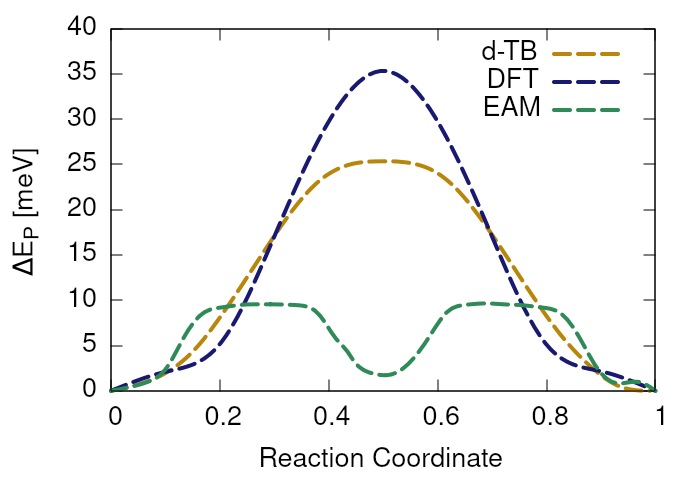
\includegraphics[width=0.5\textwidth]{Images/peierls_potential_atomistic_results.png} &
             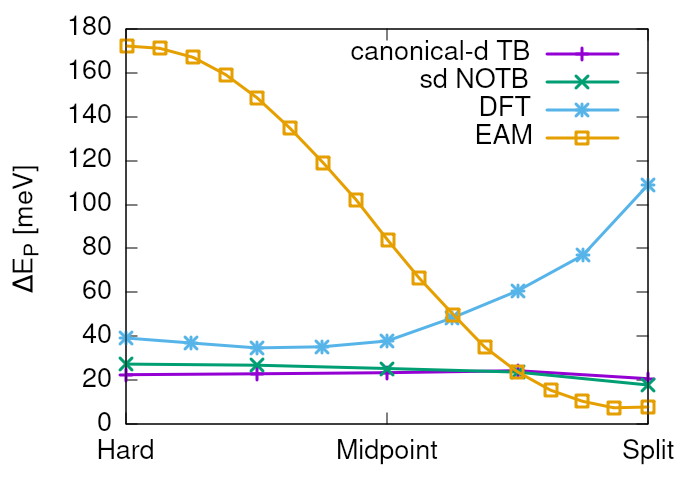
\includegraphics[width=0.48\textwidth]{Images/hard-split_transition_w_canonical.png}  \\
a) & b)\\
    \end{tabular}
\caption{Left: Peierls barriers from atomistic calculations using  canonical-$d\text{-band}$ tight-binding, DFT and the Mendelev EAM potential, plots of the corresponding dislocation pathways can be found in figure \ref{easyeasytransition}. The EAM potential of Mendelev \cite{Mendelev2003} has an unphysical well in the centre of the potential, while tight-binding and DFT produce single-humped potentials. Right: Peierls potential along the hard-split line. One can see in $s\text{-}d$ tight-binding model pathway is similar in shape to the EAM potential of Mendelev \cite{Mendelev2003}: it decreases consistently from the hard core to the split core. In DFT one finds a saddle point between the hard core and the midpoint. }
   \label{hardsplittransition}
    \end{figure}


The transitional kink shape from the \(s\text{-}d\) and \(d\text{-band}\) Peierls
potentials may differ compared to DFT, with dislocation core positions
possibly being situated closer to the split core position, similar to EAM
potentials \cite{Itakura2012,Mendelev2003}. Following the Peierls potential
along the H-S direction, as seen in figure \ref{hardsplittransition}, we see
that the Itakura potential has a saddle point minimum, which corresponds to
the dislocation core positions found upon kink-pair formation
\cite{Itakura2012}. In the \(s\text{-}d\) model, the Peierls potential decreases
monotonically along the H-S line and there is a subtle maximum found in the
\(d-\text{band}\) model. This data suggests there may be a deviation in the
dislocation path found in DFT, in moving from one peierls valley to the next along the H-S line. Atomistic calculation of
the Peierls barrier between two easy core positions in the canonical
\(d\text{-band}\) model found core positions of the transitional kink state to
go through the metastable point, similar to DFT \cite{Simpson2019}, which
suggest the deviation may not be severe. Section \ref{sec:ltmodel} discusses the
effect the Peierls potential has on the pathway taken by a
dislocation moving from one Peierls valley to the next.

\subsection{Preliminary calculations}
\label{sec:org8e4f4ec}


To validate the cluster simulation method, the excess energy, defined as the difference in energy
between a cell with a dislocation, and a perfect reference cell, was plotted as as function of
\(\ln (R/r_c)\), where \(R = R_2\) of the cluster and \(r_c = b\), as seen in
figure \ref{lnrdep}. In isotropic elasticity theory, this should give a linear dependence where the gradient
corresponds to \(\mu b^2 / 4\pi\), with the \(y\) intercept corresponding to the
core energy \(E_{\text{core}}\). This is well reproduced by our model, except at low \(\ln (R/r_c)\)
as expected, where the cell size is not large enough to accommodate for sufficient relaxation of
the dislocation core, increasing the core energy, which is not accounted for in elasticity theory.


\begin{figure}[htbp]
\centering
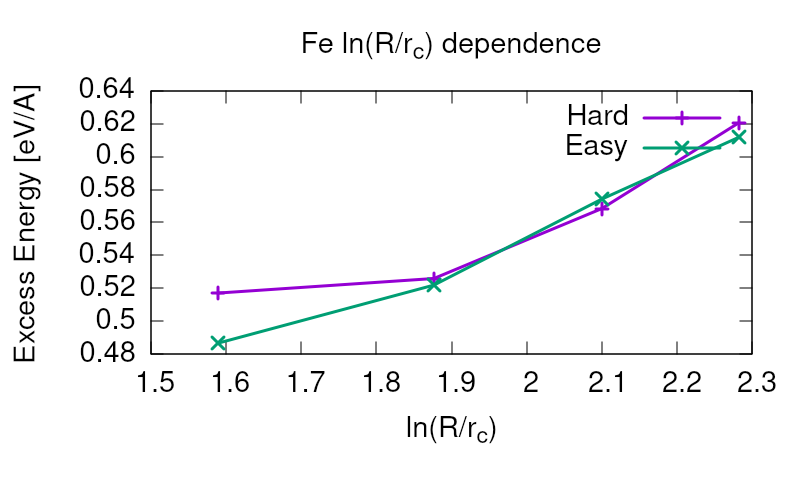
\includegraphics[width=0.7\textwidth]{/home/tigany/Documents/docs/Management/Images/img_fe_size_dependence_on_log_of_core_radius.png}
\caption{Excess energy of dislocation clusters with differing radii for both the easy and hard core configurations. The prediction from elasticity theory is given by the black, dashed line. Deviation of both cores occur when cell size is small, creating an increase in the core energy, which elasticity theory cannot account for. \label{lnrdep}}
\end{figure}




The energy cost to transform from the easy to the hard core can be estimated by
the difference in excess energies between the cores in the limit of
\(\ln (\frac{R}{R_0}) \rightarrow 0\). At the smallest measured value, one finds that the core energy
difference \(\Delta E_{\text{core}}^{\text{Easy-Hard}} = 76\) meV/b, which is in good agreement with the DFT
value of 82 meV/b \cite{Itakura2012}.


For a line tension model of a dislocation, it is necessary to
ascertain the energy, denoted \(E_{\text{L}} = E_{\text{el}} + E_{\text{core}}\) as in Proville
\cite{Rodney2009}. This can be obtained by subtracting the total
energies of relaxed dislocation configurations to obtain the core
energy.



\subsection{Fe-C binding energies}
\label{sec:orge8929d0}
\label{sec:fec_binding}

As found in DFT simulations by Ventelon \cite{Ventelon2015}, when a carbon was placed in the
vicinity of a relaxed easy dislocation core---in either of the two nearest, distinguishable,
octahedral sites---a spontaneous reconstruction of the dislocation core occurred: from easy to
hard. Upon reconstruction, the dislocation core moved to a neighbouring triangle, when looking
along the \(\langle 111\rangle\) direction, where the carbon found itself situated in the centre. This will be
called a prismatic site, as in Ventelon's paper. This confirms that both hard and easy
dislocation cores must be studied to fully understand screw dislocation behaviour in bcc iron.


The binding energies of carbon to both the hard and easy cores can be seen in table
\ref{tab:bindingenergies}, with the resulting distribution of carbon in figures
\ref{easybindingenergydist} and \ref{hardbindingenergydist}. The distribution of carbon strongly
depends on the type of core it finds itself situated near. The easy core only significantly
modifies the position of the iE1 site, to the E1 site, situated in the centre of an adjacent
triangle. All other sites are unaffected, so there is a one-to-one correspondence between all
\(\text{iE}j\) and \(\text{E}j\) sites, where \(j \in \{2\dots10\}\). There are carbon basins available close
to the triangular region containing the core, but not inside.

Carbon favours a prismatic site within the hard core (H1), which has the highest
binding energy, 1.29 eV, of all sites considered. There are no binding sites apparent in a triangular
annulus (of width \(a_{\text{bcc}}\sqrt{2}/2\)) surrounding the hard core triangle due to the
destruction/volume reduction of octahedral sites near the hard core. The initial octahedral
sites, iH1 and iH2 decay to the H1 site. Similarly, iH3 and iH4 decay to the H2 site, with iH9
and iH10 decaying to a H7 site. Relations between each of the sites is given in table
\ref{decayrelations}.


\begin{table}[htbp]
\caption{Decay relations between the initial and final sites upon relaxation of carbon intersitials around the hard core. \label{decayrelations}}
\centering
\begin{tabular}{ll}
Initial & Final\\
\hline
iH1, iH2 & H1\\
iH3, iH4 & H2\\
iH5 & H3\\
iH6 & H4\\
iH7 & H5\\
iH8 & H6\\
iH9, iH10 & H7\\
\end{tabular}
\end{table}


Note that interactions between carbon atoms around the core are not taken into account here:
figures \ref{easybindingenergydist} and \ref{hardbindingenergydist} are purely diagrammatic and not
what one expects the true distribution of carbon around a screw dislocation would be. Carbon is strongly
repulsive at first nearest-neighbour distances, which would modify each of these
distributions.


 \begin{figure}
\centering
     \begin{tabular}{l}
 	           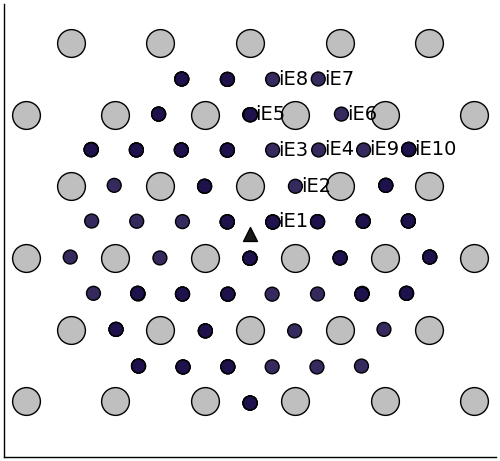
\includegraphics[width=0.7\textwidth]{Images/easy_core_fe_C_initial_positioning.png}  \\
 	           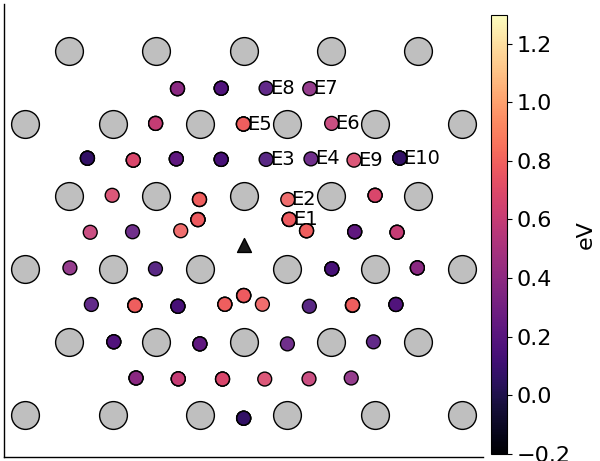
\includegraphics[width=0.85\textwidth]{Images/easy_core_fe_C_positioning_energies_e10_label.png}  \\

     	      \end{tabular}
 \caption{ Initial (top) and final (bottom) positions and binding energies (eV) of carbon around the easy core. Binding energies are not shown for the initial positions. Top: initial positions before relaxation. Bottom: final positions and binding energies after relaxation. The core was constrained by fixing the top and bottom three atoms surrounding each of the cores. As shown by Ventelon \cite{Ventelon2015}, the first and second closest octahedral sites to the hard core decay to a prismatic position inside the hard core. }
 \label{easybindingenergydist}
    \end{figure}


 \begin{figure}
\centering
     \begin{tabular}{l}
 	           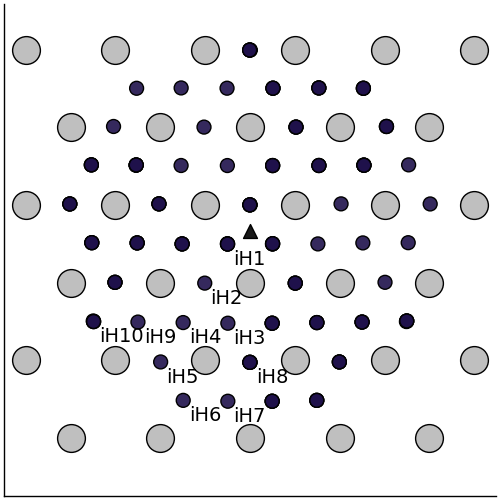
\includegraphics[width=0.7\textwidth]{Images/hard_core_fe_C_initial_positioning.png}  \\
 	           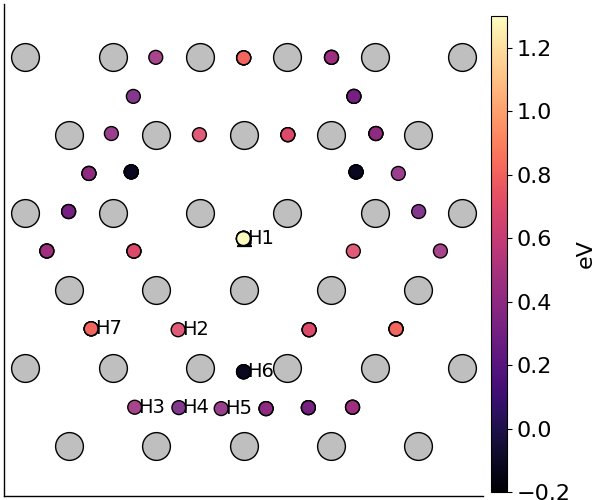
\includegraphics[width=0.85\textwidth]{Images/hard_core_fe_C_positioning_energies_h7_label.png}  \\

     	      \end{tabular}
 \caption{ Initial (top) and final (bottom) positions and binding energies (eV) of carbon around the hard core. The core was constrained by fixing the three atoms surrounding each of the cores in the top and bottom layers. As shown by Ventelon \cite{Ventelon2015}, the first and second closest octahedral sites to the hard core decay to a prismatic position inside the hard core. }
 \label{hardbindingenergydist}
    \end{figure}




    \begin{table*}
\centering
	\begin{tabular}{cccccc}
	\hline
    Site Type & distance from core [b] & $E^{z}$ [eV] & $\Delta E^{z}$ [eV] & $E_b$ [eV] & $E_b^{z}$ [eV]  \\
    	 \hline
    % 00        &                    --  &   0.203      &               0.000 &             &         --     \\
    %           &                        &              &                     &             &                \\\hline
    E1        &                   0.57 &   0.185      & 	     -0.018 &       0.793 &          0.775 \\
    E2        &                   0.70 &   0.202      & 	     -0.001 &       0.793 &          0.793 \\
    E3        &                   0.99 &   0.205      & 	      0.002 &       0.137 &          0.139 \\
    E4        &                   1.21 &   0.208      & 	      0.005 &       0.229 &          0.234 \\
    E5        &                   1.36 &   0.210      & 	      0.008 &       0.784 &          0.791 \\
    E6        &                   1.66 &   0.209      & 	      0.007 &       0.597 &          0.603 \\
    E7        &                   1.89 &   0.206      & 	      0.003 &       0.385 &          0.388 \\
    E8        &                   1.77 &   0.203      & 	      0.000 &       0.177 &          0.178 \\
    E9        &                   1.52 &   0.201      & 	      0.000 &       0.683 &          0.683 \\
    E10       &                   1.95 &   0.202      & 	      0.000 &       0.067 &          0.067 \\ \hline
    H1        &                   0.00 &   0.196      & 	     -0.006 &       1.298 &          1.291 [ 0.881\textsuperscript{a}, 0.790\textsuperscript{b}  ] \\
    H2        &                   1.19 &   0.210      & 	      0.007 &       0.691 &          0.698 \\
    H3        &                   2.12 &   0.209      & 	      0.007 &       0.461 &          0.467 \\
    H4        &                   1.91 &   0.207      & 	      0.005 &       0.311 &          0.316 \\
    H5        &                   1.80 &   0.208      & 	      0.006 &       0.403 &          0.409 \\
    H6        &                   1.40 &   0.207      & 	      0.005 &      -0.119 &         -0.114 \\
    H7        &                   1.35 &   0.206      & 	      0.006 &       0.825 &          0.819 \\

	\end{tabular}
 	\caption{Table of energies leading to the zero-point energy corrected binding energy using the cluster method for simulation of dislocation-carbon interactions. \textsuperscript{a} Tight-binding quadrupolar array results, starting from a fully relaxed easy core quadrupole extended to a depth of 3b with carbon introduced into the iH1 site in the middle layer, by both dislocations. \textsuperscript{b} DFT results of Ventelon, using the same quadrupolar configuration as in \textsuperscript{a}. In both quadrupolar simulations, carbon ended up in the H1 site.}
	\label{tab:bindingenergies}
    \end{table*}

These binding energies agree well with experiment and atomistic/elastic calculations. EAM simulations
by Clouet \cite{Clouet2008,Becquart2007} found a maximum binding energy of 0.41 eV by calculating
the elastic dipole tensor within Eshelby theory. Hanlumyuang et al. \cite{Hanlumyuang2010},
similarly conducted DFT and EAM calculations for the interaction energy 12\AA{} from the core, and
their calculations agreed with the continuum limit of Eshelby theory with a binding energy of
0.2 eV. In DFT calculations by Ventelon \cite{Ventelon2015}, the interaction energy of a carbon in a
hard core prism configuration was found to be 0.79 eV for a thickness in the \(Z\) direction of
3\(b\) (0.73eV for \(6b\))---in the convention that a positive binding energy indicates
attraction. This is significantly lower than the 1.29eV interaction energy of tight-binding.
This discrepancy can be partially explained by the fact that the cells have not been allowed to
relax with all degrees of freedom, as in the Ventelon results: the three atoms around the screw
core are fixed in \(Z\) to so the dislocation core position does not change upon
relaxation.

Repeating the calculation for the binding of a H1 carbon to a screw
dislocation using a quadrupolar array, allowing for all atoms to relax, gives a
binding energy of 0.88 eV. This agrees very well with the DFT results of Ventelon
\cite{Ventelon2015}.

A source of error for this discrepancy is likely from the fitting of the tight-binding model
itself. The Peierls barrier of this \(s\text{-}d\) model of iron, necessary for Fe-C
interactions, has been shown to be half that found in DFT \cite{Simpson2019}, but the
solution energies for Fe-C defect complexes are well described. This implies there is
insufficient repulsion between Fe-Fe species upon deformation, leading to a larger
resultant Fe-C binding energy from tight-binding.



\subsection{Carbon concentration along on line}
\label{sec:org43adba5}

The variation of carbon concentration along the dislocation line for the highest
binding energy sites of the easy and hard cores can be seen in figure
\ref{cdhardeasy}. We see at low temperatures, all dislocations are
decorated with carbon. As temperature increases, the amount of carbon
decorating the dislocations starts to decrease. Due to the lower binding
energy of carbon to the easy core, desaturation occurred at a lower
temperature compared to the hard core. Dislocation densities near the upper
bound of what has been observed in martensite, \(\rho \approx10^{15}\), reduce
the temperature at which carbon concentration starts to decrease on the
dislocation core. Lower nominal carbon concentrations cause carbon
concentrations around the dislocation to decrease at a lower temperature.

In the high-purity iron case, \(C_{\text{nom}} = 10\) appm, we find at
dislocation densities above \(\rho \approx10^{15}\), that there is a reduction
in the maximum concentration permitted in the material, with increasing
dislocation density. This is due to the fact that there is not enough carbon
for all of the dislocations, as such the concentration on the dislocation line
drops.

In the operating temperature range of \(40-90\deg\text{C} = 310-360\deg\text{K}\), we expect most hard
core sites are saturated. Given the high concentrations of the E1/E2 sites around the easy core
in this range, we expect all dislocations will be of the hard core type, due to reconstruction of
the easy core by the adjacent carbon.

\begin{landscape}
 \begin{figure}
  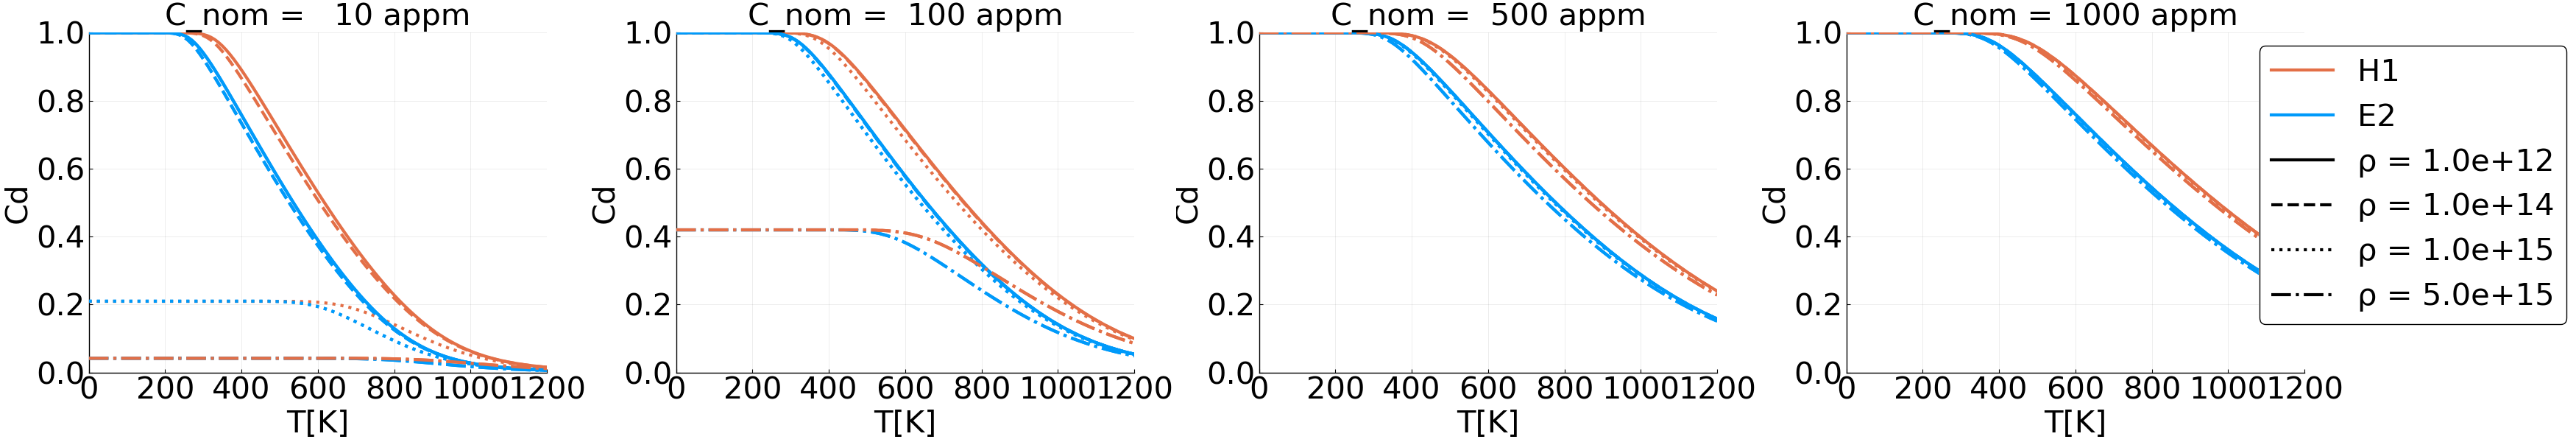
\includegraphics[width=1.6\textwidth]{Images/mcclean_isotherm_all_e2_h1.png}
   \caption{Variation of carbon concentration on the dislocation line $c_d$ for the highest-energy binding sites for the hard core (H1) and easy core (E2). Solid, dashed, dotted and dash-dotted lines correspond to dislocation densities of $1\times10^{12}$, $1\times10^{14}$, $1\times10^{15}$ and $5\times10^{15}$ respectively. The nominal carbon concentrations are 10, 100, 500 and 1000 appm from left to right, where around 1000 appm corresponds to the concentration of carbon at the solubility limit of C in ferrite: 0.02wt\%. $c_d$ and $c_{\text{bulk}}$ reached self-consistency, with an absolute tolerance of $1\times 10^{-6}$. C-C interactions were taken into account with the repulsive first-neighbour interaction energy $V_{\text{CC}}=0.30$ eV. No intersite interactions were taken into account. The maximum concentration of carbon around the easy core, drops off at a lower temperature than that of the hard core due to lower binding energy of the E$2$ site compared to the H1 site. The operating temperature is taken to be $50\deg$ C $= 320 \deg$ K.}\label{cdhardeasy}
\end{figure}
\end{landscape}





\subsection{Line Tension Model}
\label{sec:orgb8fbbf1}
\label{sec:ltmodel}

\textbf{*} Insert here what the line tension model neglects in terms of energetics \textbf{*}
\begin{enumerate}
\item Prerequisites
\label{sec:orgd6d58ad}

The \(K\) coefficient for the line tension model was calculated from atomistic simulations, using
the method of Itakura \cite{Itakura2012}, by calculation of a Hessian from the displacement of
atoms surrounding the dislocation core. Tight-binding gave \(K = 0.734\) eV\AA{}\(^{-2}\), which agrees well
with DFT, where \(K = 0.816\) eV\AA{}\(^{-2}\).


[\begin{figure}[htbp]
\centering
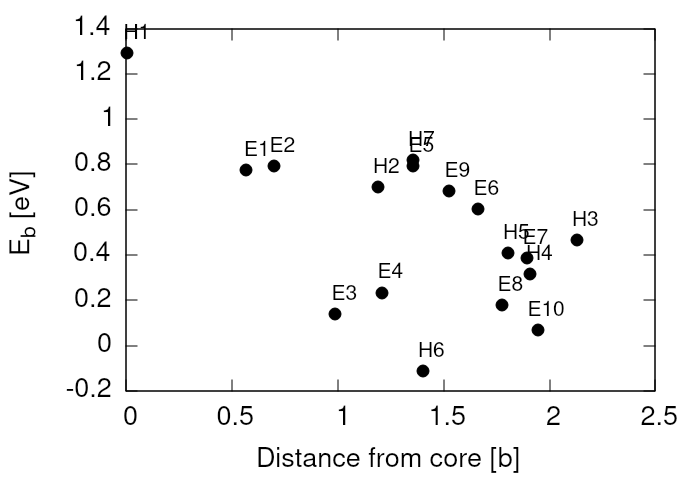
\includegraphics[width=0.7\textwidth]{/home/tigany/Documents/docs/Management/Images/fe_c_binding_energy_distance.png}
\caption{Distance dependence of the binding energies of carbon to the \(1/2\langle 111 \rangle\) screw dislocation in iron. Positive binding energies denote a favourable binding. \label{distancedep}}
\end{figure}]

Dislocation-carbon binding energies were found to decay with distance, as seen in figures
\ref{distancedep} and \ref{lorentzianfit}. A Lorentzian was fit to specific binding energies such
that a continuous function could be used to describe binding within
the line tension model. This is a purely empirical model. The
choice of sites used for the fitting is discussed in section
\ref{sec:discussion}.




\begin{figure}[htbp]
\centering
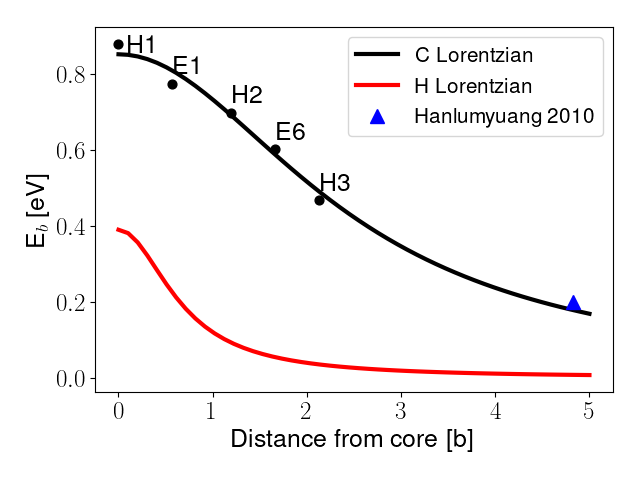
\includegraphics[width=0.7\textwidth]{iron/Images/binding_energy_dependence_C_H_lorentzian_with_scatter.png}
\caption{Parameterised distance dependence of carbon binding energies to the \(1/2\langle 111 \rangle\) screw dislocation in iron. The sites chosen to fit to were determined by those sites a prismatic carbon in a hard core configuration would find itself, if the dislocation were to move without it along the \(X = \langle\bar{2}11\rangle\) direction. The triangle, labelled Hanlumyuang, refers to the binding energy resulting from measurement of the elastic dipole tensor from DFT calculations evaluated at \(12\AA\) \cite{Hanlumyuang2010}. Binding energy of hydrogen to the \(1/2\langle 111 \rangle\) screw dislocation also shown for comparison \cite{itakura13_effec_hydrog_atoms_screw_disloc} \label{lorentzianfit}}
\end{figure}

This distance-dependence agrees well with previous calculations of the binding energy
at larger distances from the core \cite{Hanlumyuang2010}.

\item Kink-pair formation in pure iron
\label{sec:org1f635fe}

\begin{figure}[htbp]
\centering
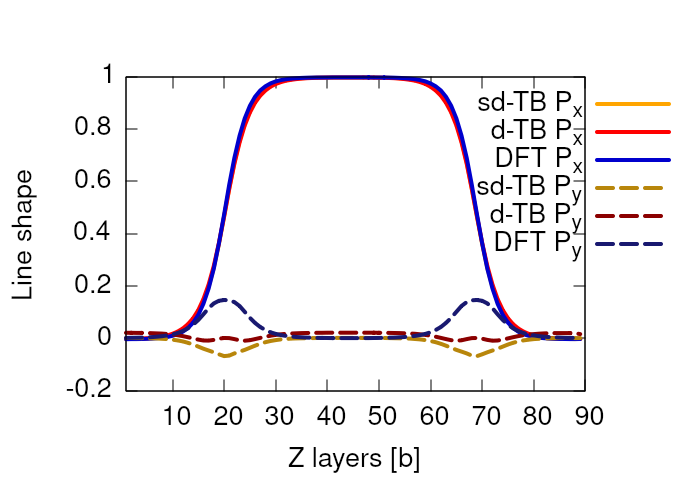
\includegraphics[width=0.7\textwidth]{iron/Images/lineshape-all_correct_gradient.png}
\caption{Core positions of the line tension model from DFT (blue) and tight-binding (yellow) for the middle image corresponding the MEP and the kink-pair formation energy. Images were relaxed using the ODE String method of Makri and Ortner \cite{Makri2019}. \(P_x\) and \(P_y\) correspond to the x/y-coordinate of the dislocation core position in each of the discretised layers of the dislocation. One finds that the kink width in tight-binding is wider than that found in DFT, which corresponds with the fact that the width is proportional to \(b\sqrt{K/\Delta E_P}\), where the reduction in \(\Delta E_P^{\text{tbe}}\) is greater than the reduction in \(K_{\text{tbe}}\).   \label{lineshape}.}
\end{figure}



In figure \ref{lineshape}, one can see the \(P_x\) and \(P_y\) core positions which
result from the highest enthalpy image of kink-pair formation for the
canonical-\(d\) and \(sd\) tight-binding models, where the DFT comparison is from
\cite{Itakura2012}. Plots of the corresponding dislocation core pathway, \(P_j =
     (P^j_x, P^j_y)\), looking down the dislocation line, are shown in
\ref{easyeasytransition}.

The \(P_x\) line shape agrees well with the DFT-based results. The kink width
was found to be slightly wider: \(W_k \sim 11b\) in tight-binding from the
line-tension model, compared to \(10b\) in DFT and atomistic tight-binding
results \cite{Simpson2019}. The larger width from tight-binding compared to
DFT results from the width being proportional to \(b\sqrt{K/\Delta E_P}\)
\cite{Itakura2012}, with the discrepancy between the \(K^{\text{tbe} }\) and
\(K^{\text{DFT} }\), being smaller than that of the Peierls
potential. Differences in the \(P_y\) line shape are noticeable, with the
canonical-\(d\) model reproducing the result closest to the DFT \(P_y\) line
shape.

The differences in line shapes manifest themselves clearly in
plots of the dislocation pathway, figure \ref{easyeasytransition}, where we
see the path a dislocation takes looking down the dislocation line.
The core pathway dips below the midline in both the
\(d\) and \(sd\) models, with a more pronounced effect being shown by the \(sd\)
model. Apart from this discrepancy, we see there is good agreement between
tight-binding to DFT when compared to the EAM potential of Mendelev
\cite{Mendelev2003} in which we see a path which passes close to the split-core
position. This is expected due to the low value of the Peierls potential of
the EAM, as seen in figure \ref{hardsplittransition}.



\begin{figure}[htbp]
\centering
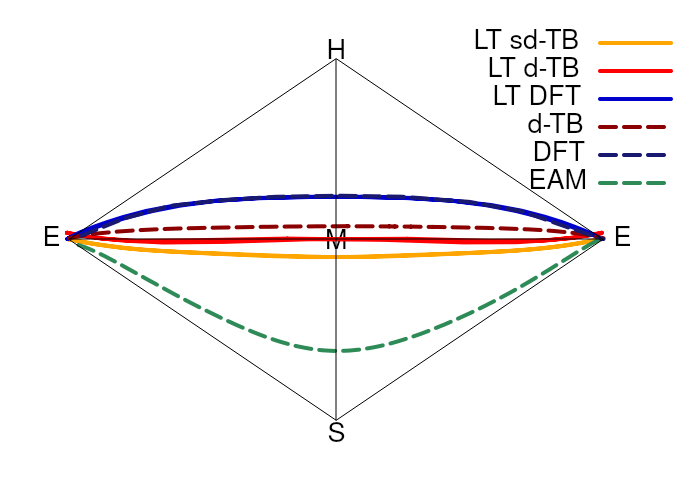
\includegraphics[width=0.7\textwidth]{iron/Images/easy-easy_transition_pathway_combined_dTB_sdTB_DFT_EAM_dotted_smooth_colour.png}
\caption{Comparison of minimum energy pathways from different atomistic calculations to the line-tension model. Dashed lines correspond to atomistic calculations. Solid lines are results from the line-tension models. Tight-binding follows a pathway much closer to that of DFT. EAM potentials predict that the dislocation core goes to the split core and then back to the easy core. Even though the Peierls landscape found in tight binding has similar characteristics to the EAM in terms of the energetic ordering of different core states, the description of the minimum energy pathway of the \(1/2\langle 111 \rangle\) screw dislocation as it moves between core positions is in good agreement with DFT. \label{easyeasytransition}}
\end{figure}



The kink-pair formation enthalpies obtained from the tight-binding models can
be found in table \ref{kink-pair_formation_enthalpy_pure}. Tight-binding
underestimates the kink-pair formation enthalpy by \(0.18\) eV, in comparison to
DFT. This can largely be attributed to the difference in Peierls potentials
between DFT and tight-binding.

\begin{table}[htbp]
\caption{Kink-pair formation energies between DFT, and the two flavours of tight-binding used with the line-tension model \label{kink-pair_formation_enthalpy_pure}.}
\centering
\begin{tabular}{ll}
Method & \(H_{\text{k}}\)\\
\hline
DFT & 0.71 eV\\
TB (sd-non-orthog.) & 0.56 eV\\
TB (d-orthog.) & 0.53 eV\\
\end{tabular}
\end{table}


\item Kink-pair formation enthalpy with a single carbon
\label{sec:orgaacc02e}

To understand how kink-pair nucleation is affected by carbon, one
can study the formation of a kink-pair but with the
additional interaction of a single carbon ahead of the dislocation.

We place carbon in the E1 site, the highest binding energy site of carbon to
the easy dislocation core. The carbon is fixed in place during kink-pair
formation, as such we are assuming a regime in which the dislocation
velocity is much greater than the diffusion of carbon. Carbon-dislocations
interactions are only permitted between the dislocation segment closest to
the carbon.


    \begin{figure}
\centering
	\begin{tabular}{r}
		      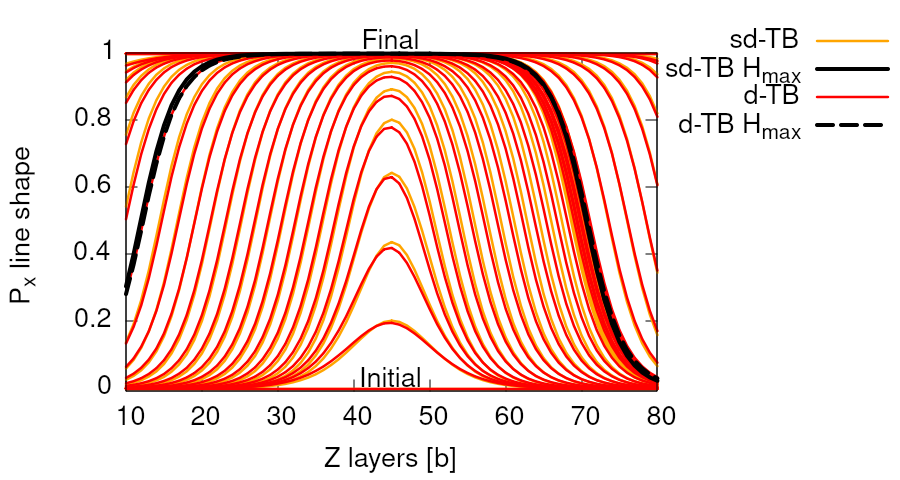
\includegraphics[width=0.75\textwidth]{Images/lineshape_no_carbon_sd_dTB_off_kilter_hmax_label.png} \\
		      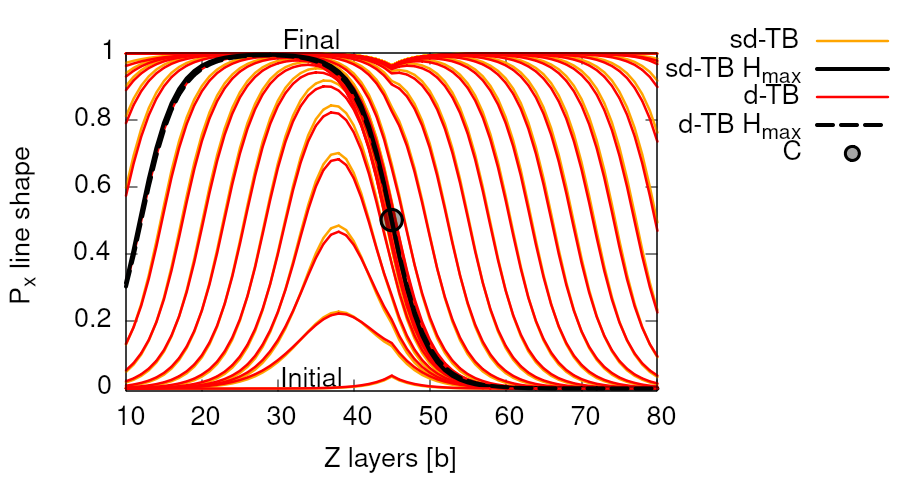
\includegraphics[width=0.75\textwidth]{Images/lineshape_with_carbon_sd_dTB_off_kilter_hmax_label.png}  \\

		 \end{tabular}
    \caption{ Comparison of $P_x$ lineshapes for the $sd$ and $d$ models in pure iron (top) and iron with a single carbon interacting with the central dislocation segment in E1 site (bottom). The highest enthalpy images, $H_{\text{max}}$, for each of the models are shown in black. In pure iron, the $d$ model lineshapes are offset from the $sd$ due to the different Peierls potentials involved. With carbon along the path of migration, we find the dislocation intersects the solute, due to its large binding energy.}
    \label{fig:alllineshapes}
       \end{figure}


\(P_x\) line shapes obtained during kink-pair formation can be seen in figure
\ref{fig:alllineshapes}. The addition of carbon causes a cusp in the
dislocation line towards the carbon in the initial and final images, due to
the reduction in potential the central dislocation segment experiences due
to carbon interaction. As the dislocation bows out to form a kink pair, the
cusp becomes less prominent. As we reach the transition state, the dislocation
image intersects the carbon position, to minimise energy.

The pathway corresponding to the highest enthalpy image, can be seen in
figure \ref{fig:pathwaysinglec}. Looking along a direction, we see the path a
dislocation takes in going between adjacent peierls valleys is asymmetric,
as expected due to the due to the strong binding of carbon.

These features agree very well with the line tension model in Itakura
\cite{itakura13_effec_hydrog_atoms_screw_disloc}, focussing on the case of
dislocations undergoing kink-pair formation in the presence of a single
hydrogen atom.

\begin{figure}[htbp]
\centering
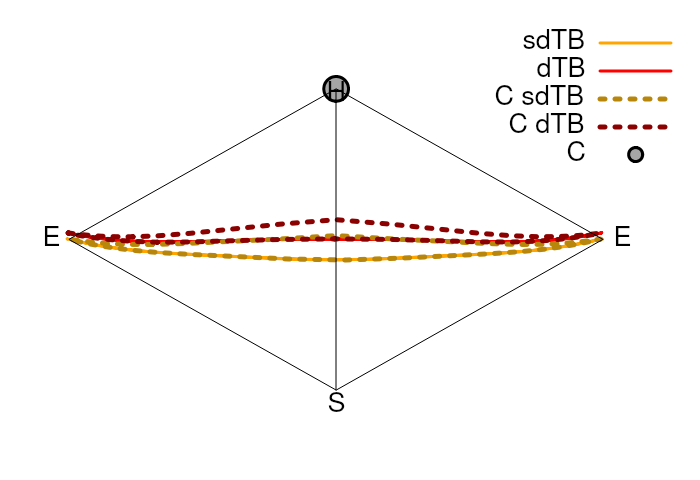
\includegraphics[width=0.8\textwidth]{iron/Images/pathway_single_carbon_sd_d.png}
\caption{The migration path of the highest enthalpy images for both the \(sd\) and \(d\) tight-binding models with a single carbon in an E1 site. Carbon causes a deviation of the kink-pair formation path from the pure iron case (solid lines), due to carbon-dislocation binding. \label{fig:pathwaysinglec}}
\end{figure}


\begin{figure}[htbp]
\centering
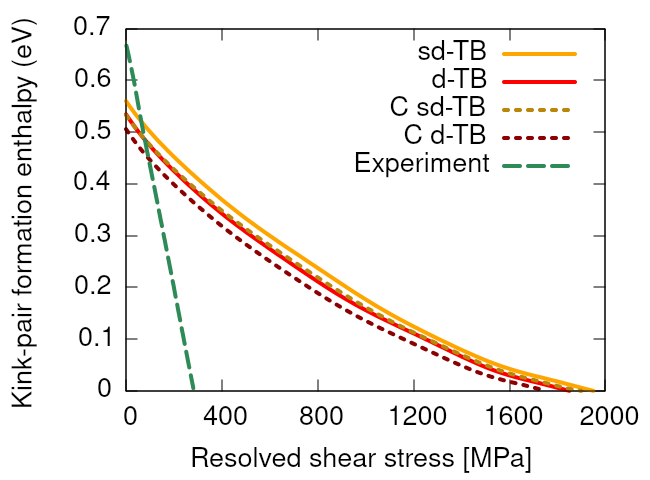
\includegraphics[width=0.8\textwidth]{iron/Images/kink-pair_formation_enthalpies_dTB_sdTB_2000_big.png}
\caption{Dependence of the kink-pair formation enthalpy with increasing stress on the \([111](1\bar{1}0)\) direction. Solid lines: pure iron. Dotted lines: carbon ahead of the dislocation line in an octahedral site. Experimental data taken from Spitzig \cite{Spitzig_1970}. \label{kinkpairstress}}
\end{figure}



The kink-pair formation enthalpy of \(sd\) and \(d\) iron models, in both pure
iron, and with carbon ahead of the dislocation line are shown in figure
\ref{kinkpairstress}. The shape agrees well with results of the line tension
model of Itakura \cite{Itakura2012}, and from atomistic calculations of EAM
\cite{Proville2012} and GAP \cite{Maresca2018} Fe potentials. We find that
carbon produces a consistent reduction of \(\sim 25\text{meV}\) to the
kink-pair formation enthalpy when placed ahead of the dislocation line. The
reduction is surprisingly small compared to the effect of hydrogen
interaction with dislocations
\cite{itakura13_effec_hydrog_atoms_screw_disloc}, which gives a reduction of \(\sim 110 \text{meV}\). The discrepancy between carbon and hydrogen is due to
the more gradual decrease of the carbon-dislocation interaction---over the
distance between the initial and transition states---compared to the
hydrogen-dislocation interaction, as shown in figure
\ref{lorentzianfit}. Comparing the two interaction functions, we have at the
peierls valley \(P_{\text{disl}}=(0,0)\), and \(P^{\text{H}} = P^{\text{C}} =
     (1.17 \AA, 0.68 \AA)\) giving a distance \(d = 0.54b\) between the dislocation and
the solute. The difference in the interaction energy for a dislocation
segment in the final position in interaction for hydrogen \(\Delta
     E_b^{\text{H}} = E_b(\text{H},0) - E_b(\text{H},0.54b) = 150\) meV, whereas
for carbon we have \(\Delta E_b^{\text{C}} = E_b(\text{C},0) - E_b(C,0.54b) =
     40\) meV.


Due to the longer range of the interaction function, we expect that a single carbon
will provide comparable decreases to the kink-pair formation up to distances up to 5b,
if placed ahead of the dislocation line. At equilibrium, where carbon exhibits
long-range ordering along the dislocation line in the H1 and H2 sites \cite{Luthi2019},
we can expect a decrease in the kink-pair formation enthalpy. Line-tension simulations in
ordered carbon environments are necessary to account for this properly. We can approximately
treat some of these effects using an effective carbon-dislocation interaction
along the dislocation line during kink-pair formation, as shown in section
\ref{sec:kinkpairformationequib}.



The stress at which the kink-pair formation enthalpy becomes zero is the Peierls
stress. In the zero temperature limit, we can approximately account for quantum
effects, such as tunnelling and zero-point energy, by subtracting the Wigner
correction, determined by quantum transition state theory
\cite{Proville2012,Henkelman2006}, from the kink-pair formation enthalpy. Calculating
this correction within atomistic tight-binding simulations is currently
intractable. The correction has been calculated using the Mendelev EAM potential
\cite{Mendelev2003} for a screw dislocation undergoing kink-pair nucleation
\cite{Proville2012}. The Wigner correction obtained is 0.09eV. We find find that the
Peierls stress obtained for both the \(sd\) and \(d\) models is \(\approx1.2\text{GPa}\), see table
\ref{wignercorrection}.


\begin{table}[htbp]
\caption{Peierls stress of screw dislocation taken from the line tension model with the effect of the correction to the Peierls stress from quantum effects, estimated by Proville \cite{Proville2012}. DFT results are found from papers of Itakura and Krach \cite{Itakura2012,Kraych2019}, where Itakura \emph{et al.} used a DFT-derived line-tension model, and Kraych used DFT NEB calculations. \(^{*}\) corresponds to use of Itakura DFT data in this implementation of the line-tension model.  \label{wignercorrection}}
\centering
\begin{tabular}{lrr}
Model & Peierls Stress [GPa] & Peierls Stress with Wigner correction [GPa]\\
\hline
sd-TB & 1.95 & 1.35\\
C sd-TB & 1.90 & 1.30\\
\hline
d-TB & 1.85 & 1.30\\
C sd-TB & 1.75 & 1.20\\
\hline
DFT [Kraych, 2019] & 2.00 & \\
DFT [Itakura, 2012] & 1.00 [*2.10] & \\
\end{tabular}
\end{table}



Discrepancies in the kink-pair formation enthalpy compared to experimental
measurements of Spitzig \cite{Spitzig_1970}, can be attributed to multiple
sources. In bcc metals, experimental measurements of the CRSS, which can be
linked to the kink-pair formation enthalpy, are thought to measure the
stress required to operate Frank-Read sources which have been blocked due to
the back stress of generated screw dislocations \cite{Groger2007}. As mixed
dislocations bow out from the source, long screw segments form---due to the
higher mobility of mixed/edge character segments compared to screw
segments. Between the source and the screw dislocations, there are non-screw
dislocations, stresses from which act in conjunction with applied stress to
reduce the necessary CRSS by 2-3 times. As such the enthalpy barrier
obtained from the experimental CRSS measurements of Spitzig, cannot be
directly compared to the true kink-pair formation enthalpy necessary for a
single screw dislocation to undergo thermally-activated movement.

\item Kink-pair nucleation rate
\label{sec:org1daff70}
\label{sec:kink-pair_nucleation_rate}

One can use an Arrhenius law to calculate the attempt frequency of a process given an
energy barrier \(E_{\text{barrier} }\) \cite{Henkelman2000},

\begin{equation} \label{eq:jumprate}
   \nu ( E_{\text{barrier}},T ) = \nu_0 \exp \big( - \frac{ E_{\text{barrier} }}{ k_{\text{B}} T} \big),
\end{equation}

where \(\nu_0\) is an initial attempt frequency.

The kink-pair nucleation rate of a dislocation of length \(N_d\) burgers vectors is
given as \cite{itakura13_effec_hydrog_atoms_screw_disloc}:


\begin{equation} \label{eq:kinkrate}
\nu_{\text{d}} = \nu ( H_k(\sigma),T ) N_d,
\end{equation}

where \(H_k(\sigma)\) is the kink-pair formation
enthalpy. Experimental results of \emph{in situ} straining of Fe from Caillard
\cite{Caillard2010}, enable calculation of the attempt frequency for stable
kink-pairs: assuming \(b = 2\mu\text{m}\), \(T=\) 300K and an applied stress of
33MPa one obtains \(\nu_{\text{d} } = 81s^{-1}\).

There will be an enhancement of the rate due to carbon occupying sites ahead
of the dislocation. Given a concentration of carbon on the dislocation line, \(c_d\), we
have in the sites ahead, the rate enhancement factor is

\begin{equation} \label{eq:enhancementfactor}
  f_r(c_d,\Delta H_{k},T) = 1 + c_d W_k \{  \exp( \Delta H_{k}/k_{\text{B}}T ) - 1 \}.
\end{equation}

where \(\Delta H_{k} = H_k - H_k^{\text{C}} =\) 25meV and \(W_k \sim 10b\) is the
kink-width. Assuming \(T=300\) K, and assuming the concentration of carbon is
\(c_d^{\text{E2}}\), we obtain enhancement factors as
shown in table \ref{rateenhancement}.


\begin{table}[htbp]
\caption{Enhancement factors to the kink nucleation rate and corresponding critical temperatures. \(c_d\) was taken as the value reached from self-consistency at T=300K, at a dislocation density of \(\rho = 10^{15}\), as seen in figure \ref{cdhardeasy}. Kink-pair nucleation rate enhancements steadily increase until concentrations at which all dislocations are decorated with carbon, in the cases of \(C_{\text{nom}} \geq 500\) appm. The critical temperatures are all well above operating temperature, so we can expect rate enhancements during operation. \label{rateenhancement}}
\centering
\begin{tabular}{rrr}
\(c_{\text{nom}}\) [appm] & \(f_r\), Rate Enhancement factor & \(T_{\text{U}}\) [K]\\
\hline
10 & 4.4 & 745\\
100 & 7.9 & 1329\\
500 & 17.3 & 3043\\
1000 & 17.3 & 3043\\
\end{tabular}
\end{table}


These rate enhancements are an order of magnitude less compared to what one finds with
hydrogen in iron \cite{Simpson2019}, due to the small reduction to the kink-pair
formation enthalpy with carbon. However, this only accounts for a the effect of a
single carbon just ahead of the core. Complex ordering phenomena of carbon has been
found along the screw dislocation in Fe, which could enhance the kink-nucleation rate
\cite{Luthi2019}. Ising models parameterised on \emph{ab-initio} data give equilibrium
concentrations of different carbon trap sites along the dislocation core, accounting
for carbon-carbon repulsion. They predict H1 and H2-type sites in adjacent
layers can have concentrations which are \(\sim 1.0\) and \(\sim 0.25\) respectively, when
the nominal carbon concentration is 100 appm. The effect of multiple
carbon-dislocation interactions on the the kink-pair formation enthalpy has yet to be
determined, but we expect \(\Delta H_{\text{k}}\) and therefore the rate enhancement, to increase.

Significant enhancement of the nucleation rate occurs when the rate enhancement factor
is on the order of \(f_r \sim 1\) or greater. Defining \(c_d^E = \frac{1}{W_k \{\exp(
    \Delta H_{k}/k_{\text{B}}T ) - 1 \}}\), one can impose a condition when \(c_d^E > c_d\),
defining a critical temperature \(T_{\text{U}}\) after which these enhancements are not
deemed important. See table \ref{rateenhancement}. All the critical temperatures
are found to be above operating temperature.





The diffusion coefficient of carbon in bcc Fe has been calculated in DFT as
\(D_{\text{C}} = 1.44 \times10^{-7} \text{m}^2\text{s}^{-1}\), which agrees well with
experiment \cite{Jiang2003,daSilva1976}. The attempt frequency is related to the
diffusion coefficient by \(\nu_0 = 6D_0 / a^2\) \cite{Ramasubramaniam2008}, which gives
the attempt frequency of carbon as \(\nu_{\text{C}}^0 = 1.0 \times10^{13} s^{-1}\)
\cite{Nematollahi2016}. The migration energy barrier of carbon in bcc Fe was found to be
\(E^{\text{m bulk}}_{\text{C}} = 0.87 \text{eV}\) in DFT calculations.

From the experimental rate of stable kink-pair nucleation \(\nu_{\text{d}} = 88 s^{-1}\)
from Caillard, we can estimate the prefactor \(\nu_{\text{d}}^0 = 0.99 \times
    10^8\text{s}^{-1}\) using experimental the kink-pair formation enthalpy at 33 MPa
\cite{itakura13_effec_hydrog_atoms_screw_disloc}.

The average velocity associated with a process undergoing thermal activation of a
barrier is given by \(\bar{v} = d_{\text{barrier}}\nu\), where \(d_{\text{barrier}}\) is
the distance between the the initial and final states of the barrier. For dislocations
we use \(d_{\text{d}} = a\sqrt{2/3}\) is the distance between Peierls valleys for
kink-pair formation and \(d_{\text{C}} = 1.2\AA\) is the distance between octahedral
sites which carbon can jump to. As these distances are on the same order of magnitude,
we omit the explicit calculation of velocities for clarity, using the attempt frequencies for comparisons.

At \(T=300 \text{K}\) and \(C_{\text{nom}} = 1000 \text{appm}\), around the solubility
limit of carbon in ferrite (0.02 wt\% C), we have \(\nu_{\text{C}}(E^{\text{m
    bulk}}_{\text{C}},300) = 2.4\times 10^{-2} s^{-1}\), with \(f_r(1000
    \text{appm})\nu_{\text{d}}(H_{\text{k}},300) = 1.7 \times 10^{-1} s^{-1}\). This shows
that in the bulk, carbon cannot be assumed to move with the dislocation, as the
attempt frequency of carbon is an order of magnitude less than that of kink-pair
formation.

However, it has been shown in EAM calculations that much lower carbon migration
barriers exist in the vicinity of a screw dislocations \cite{Nematollahi2016}. The
migration barrier of carbon is reduced to \(E^{\text{m disl.}}_{\text{C}} = 0.2
    \text{eV}\). Using this value we obtain \(\nu_{\text{C}}(E^{\text{m
    disl.}}_{\text{C}}, 300) = 4.4 \times 10^{9} s^{-1}\). We see that the average carbon velocity
will be much greater than that of dislocations undergoing thermally-activated movement, as
such we can assume that in the high-mobility zone, that carbon is able to move with
dislocations.


The timescale of carbon redistribution with dislocation movement remains negligible as
long as the kink-pair formation enthalpy with carbon \(H_{\text{k}}^{\text{C}}(\sigma)\)
is greater than the migration barrier energy in high mobility zone:
\(H_{\text{k}}(\sigma) - \Delta H_{\text{k}}^{\text{C}}(\sigma) >
    E^{\text{m}}_{\text{C}}\). Using this value, we can obtain an upper critical stress
\(\sigma^{\text{U}}_c \sim 210 \text{MPa}\), above which carbon cannot enhance
dislocation mobility, as it cannot catch up with the dislocation.

\item Kink-trapping
\label{sec:org6713796}

Kink-trapping is the energetic barrier to kink-migration along the dislocation line
due to the change in binding energy of a kink sweeping past a defect. The
kink-trapping effect due to carbon can be estimated as follows
\cite{itakura13_effec_hydrog_atoms_screw_disloc}. If a
kink-pair were to form with a carbon in an E1 site behind the dislocation, the carbon-dislocation binding
energy will change. We can assume carbon remains in its
site upon movement: the barrier to kink-migration has been shown to be small
\cite{itakura13_effec_hydrog_atoms_screw_disloc,Simpson2019,Gong2020}, as such kink-migration is
orders of magnitude faster than that of carbon diffusion.

As the kink sweeps past, the E1 site becomes an E6 site, resulting in a
difference in binding energy of \(\Delta E_b^{\text{E}1\rightarrow
      \text{E}6} = 0.775 - 0.603 = 172\) meV. This trapping effect is expected to
decrease with applied stress, as shown in Itakura, but this is left for
future work.

The kink-trapping effect of carbon will be pronounced when a dislocation
moves from its equilibrium position as there will be multiple carbons along
the dislocation line \cite{Luthi2019}. This effect has yet to be estimated.

This is an important effect to account for, as solute drag has been shown to reduce
the kink-migration velocity sufficiently such that
jogs can form on dislocations due to the collision of kinks on different glide
planes causing pinning and the formation of edge dipoles seen in experiment \cite{Gong2020,Katzarov2017b}.
\end{enumerate}

\subsection{Line-tension equilibrium conditions}
\label{sec:orga9d5b33}

\begin{enumerate}
\item Dynamics of straight 1/2\(\langle 111 \rangle\) screw dislocation
\label{sec:org9233989}

Figure \ref{fig:straighttbequib} shows the potential a straight screw
dislocation experiences as it moves between peierls valleys in an
equilibrium carbon environment, allowing carbon to redistribute between trap
sites upon glide. The potential a dislocation experiences decreases as
carbon concentration is increased. This is due to the stabilisation of the
hard core position with increases in carbon content. With stabilisation,
E1/2 sites are distorted into H1 sites. At concentrations \(\gt
     20\text{appm}\), the mean carbon-dislocation interaction energy becomes
greater in magnitude than the bare Peierls potential, resulting in a
potential well.


\begin{figure}[htbp]
\centering
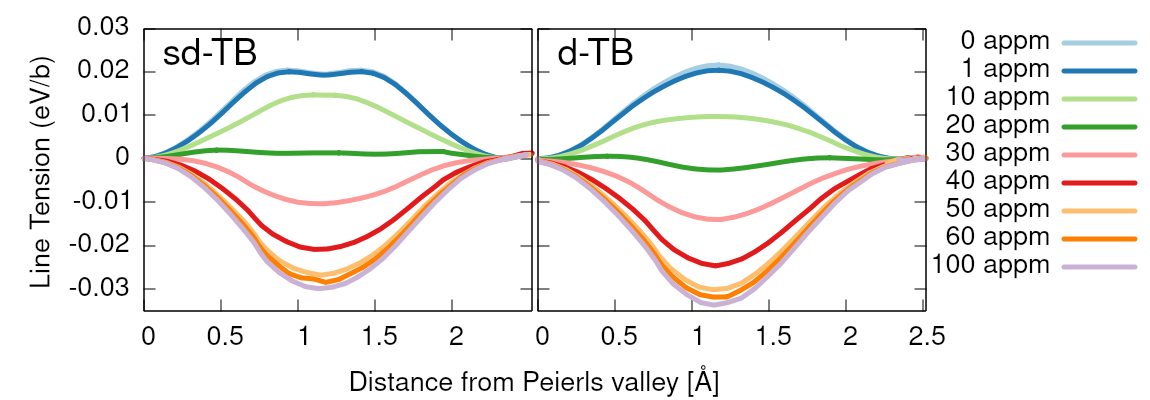
\includegraphics[width=.9\linewidth]{iron/Images/straight_line_enthalpies_equib_both.png}
\caption{Enthalpies of straight screw dislocation in the line-tension model in an environment of carbon with concentrations determined by thermodynamical mean field model. Carbon concentration on the dislocation on the dislocation line is in equilibrium with the bulk according to the concentration given by the H1 site, where carbon is able to redistribute between the sites according to Maxwell-Boltzmann statistics. \label{fig:straighttbequib}}
\end{figure}



Figure \ref{fig:straighttbstatic} shows the case where the concentration of
carbon is not allowed to equilibrate: simulating the limit of rapid glide,
where the occupancies of carbon in all trap sites is fixed to the value
determined at the initial easy-core configuration of the straight
dislocation. The occupancies decrease rapidly with distance from the
core. As such, the energy a straight dislocation experiences, relative to the initial
dislocation position, increases with
distance from the Peierls valley, due to a reduction in the
dislocation-carbon interaction energy from a lack of carbon occupancy.


\begin{figure}[htbp]
\centering
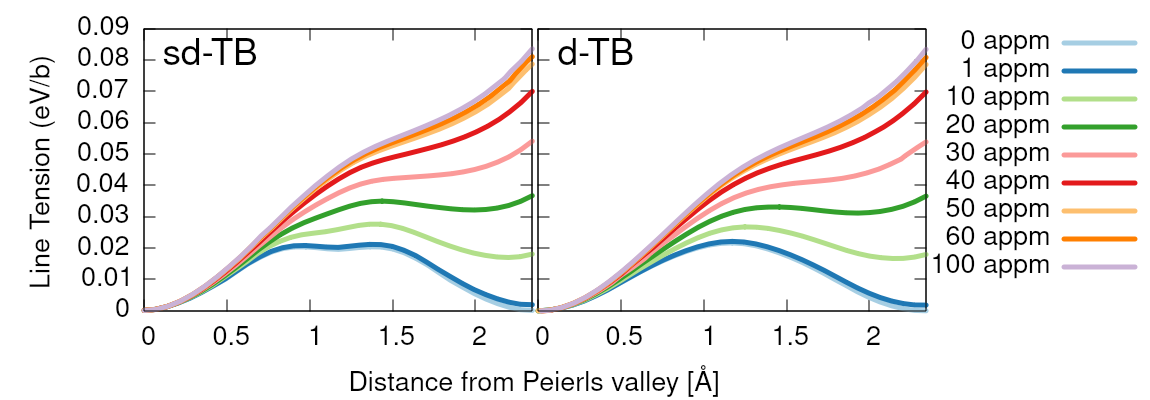
\includegraphics[width=.9\linewidth]{iron/Images/straight_line_enthalpies_static_both.png}
\caption{Enthalpies of straight screw dislocation in the line-tension model in an environment of carbon with concentrations determined by thermodynamical mean field model. Concentration of carbon in each of the sites is fixed to its initial value, simulating the limit where carbon does not have time to equlibriate with dislocation movement. \label{fig:straighttbstatic}}
\end{figure}

In reality, we have a situation which is between the two. This can be accounted for by
a continuity term which is dependent on dislocation velocity \cite{Gong2020}.

\item Dynamics of kink-pair formation in equilibrium
\label{sec:org0f3f659}
\label{sec:kinkpairformationequib}
The line-tension upon kink-pair formation, in the limit of slow glide, can
be seen in figure \ref{fig:kinkpairequib}. As the hard core is stabilised with
increasing carbon content, the line tension decreases, due to the negation
of the bare Peierls potential with increasing carbon-dislocation interaction
energy. At nominal concentrations greater than 20 appm, the string method
finds lower energy dislocation configurations away from the straight initial
easy core position favoured at lower concentrations.

\begin{figure}[htbp]
\centering
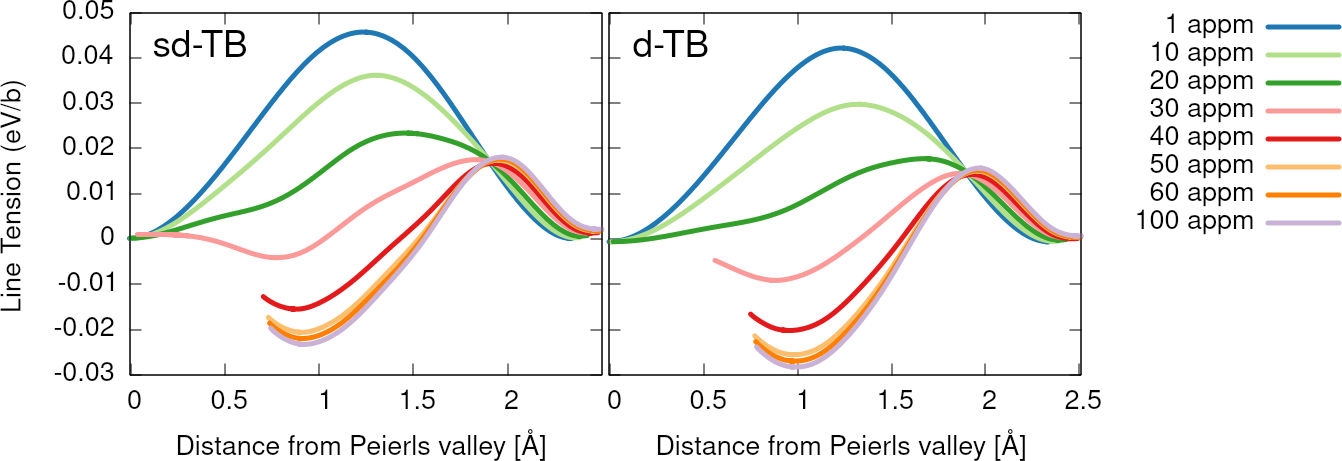
\includegraphics[width=1.\textwidth]{iron/Images/kink-pair_equilibrium_combined_moving_sites.png}
\caption{Enthalpies of the maximum enthalpy images upon kink-pair formation with increasing carbon content. Carbon interaction causes a reduction in the enthalpy barrier as due to the negation of the effect of the bare Peierls potential. As the nominal carbon concentration passes 20 appm, the hard core is stabilised, thus causing the string method algorithm to find a global minimum closer to the hard core position. \label{fig:kinkpairequib}}
\end{figure}


With increasing carbon concentration, both tight-binding models exhibit a
deviation of the maximum enthalpy pathway towards the hard core, as shown in figure
\ref{fig:kpequibpath}. At each concentration, the path a dislocation takes in the \(d\)
tight-binding model is closer to the hard core, due to the morphology of its
peierls potential.


\begin{figure}[htbp]
\centering
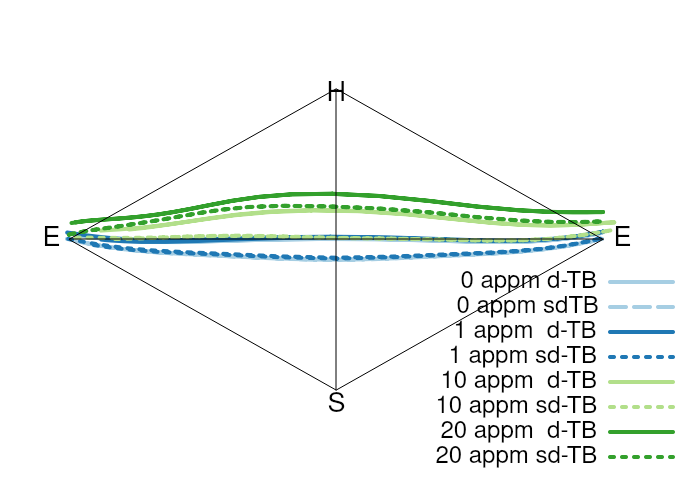
\includegraphics[width=0.8\textwidth]{iron/Images/pathway_equilibrium_sdTB_dTB_20appm_all.png}
\caption{Maximum enthalpy pathways found upon kink-pair formation in an environment of carbon for both tight-binding models at different nominal carbon concentrations. Concentrations shown are before the easy core becomes unstable. With an increase in carbon content, path starts to deviate towards the hard core. \label{fig:kpequibpath}}
\end{figure}

The lineshapes of the \(P_x\) dislocation coordinate on kink-pair formation broaden with carbon
content due to the attraction of the dislocation line to carbon sites.

\begin{figure}[htbp]
\centering
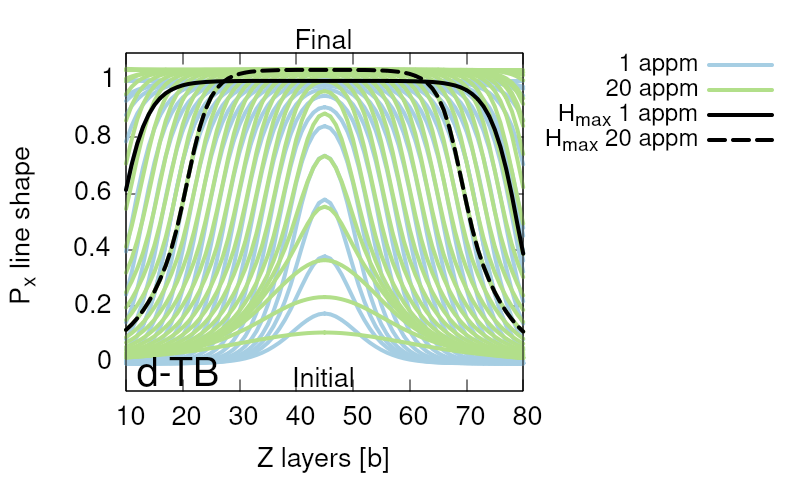
\includegraphics[width=0.9\textwidth]{iron/Images/lineshapes_dtb_moving_sites_labelled18.png}
\caption{\(P_x\) lineshape comparison of differing concentrations of the canonical-\(d\) tight-binding model.}
\end{figure}


\begin{figure}[htbp]
\centering
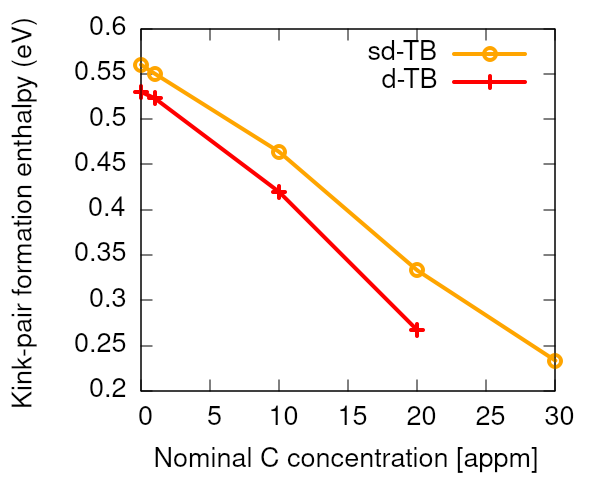
\includegraphics[width=0.7\textwidth]{iron/Images/kink-pair_formation_equilibrium_sdtb_dtb_30appm.png}
\caption{Kink-pair formation enthalpy dependence on nominal carbon concentration without the application of stress. There is a consistent decrease in the mean kink-pair formation enthalpy with carbon content.}
\end{figure}

The kink-pair formation enthalpy in an effective carbon concentration can be
seen to decrease with increasing carbon content. At concentrations greater
than 20 appm, the hard core is stabilised. Line-tension calculations of the
kink-pair formation of a dislocation moving from the stabilised hard
core to an adjacent hard-core position are necessary to ascertain the
kink-pair formation enthalpy at higher carbon contents. We expect, as
was seen in self-consistent calculations of the kink-pair formation enthalpy
in hydrogen, that the trend will be reversed: the kink-pair formation
enthalpy will increase with carbon content, once the hard core has been stabilised.


One can see the effect that these mean enthalpies have on the kink-pair nucleation
rate. Using the results of the kink-pair formation enthalpy from the canonical-\(d\)
tight-binding model, and using equations \eqref{eq:kinkrate} and \eqref{eq:jumprate}
we have the rates as shown in table \ref{eqkinkrate}. The rate enhancement factor is not
included here as the concentration term is taken into account in the
kink-pair formation calculation itself.

\begin{table}[htbp]
\caption{Kink-pair nucleation rate in an environment of carbon using the results of the canonical \(d \text{-band}\) model, using from equations \eqref{eq:kinkrate} and \eqref{eq:jumprate} \label{eqkinkrate}}
\centering
\begin{tabular}{rr}
\(c_{\text{nom}}\) [appm] & \(\nu^{\text{d}}\)\\
\hline
10 & 8.7\\
20 & 2881.8\\
\end{tabular}
\end{table}


Allowing carbon to equilibrate between trap sites during kink-pair formation, we see a
large enhancement to the kink pair nucleation rate, increasing dislocation
velocity. Carbon remains with screw dislocations upon movement, due to the low barrier
to migration in the high-mobility zone resulting in a velocity orders of magnitude
greater than that of dislocation motion. The analysis shown here is approximate. A
more complete description necessitates a self-consistent treatment of the kink-pair
formation enthalpies, as \(H_{\text{k}} = H_{\text{k}}(\bar{v}_{\text{d}})\) and
\(\bar{v}_{\text{d}} = \bar{v}_{\text{d}}(H_{\text{k}})\). This is left for future work.
\end{enumerate}




\subsection{Diffusion Barriers}
\label{sec:orgbd62493}

The diffusion barriers of carbon close to the easy core have been found to decrease---for some
transitions---from 0.87eV for bulk diffusion, down to barriers around 0.2eV
\cite{Nematollahi2016}. In the calculations shown in section \ref{sec:kink-pair_nucleation_rate}, we
see that carbon is able to keep up with the dislocation in a range of moderate velocities only if this
diffusion barrier is lowered to such a level.

However, the predictive power of the EAM potential used to obtain these barriers is limited. The
Mendelev EAM potential used in these calculations is unable to reproduce: the 2D Peierls
potential, which is double-humped, instead of single-humped \cite{Mendelev2003}; the metastable
hard core structure, which exibits a spontaneous reconstruction to the hard core from the easy core and, the binding energies of
carbon close to the dislocation core---being roughly half that found in Ventelon and this work
\cite{Becquart2007,Ventelon2015}. These discrepancies are likely due to the inherent lack of
quantum mechanics in the EAM description of bonding, which seems necessary for an accurate
description of energetics close to the dislocation core. As such, it remains to be seen if the
diffusion barriers, and consequent diffusion rates obtained from this EAM potential are faithful.

As seen in figure \ref{cdhardeasy}, at moderate dislocation densities, we expect all dislocations
to be decorated with carbon, and be of hard-core type. As such, it is important to ascertain the
diffusion barriers of carbon around the hard core, as it is the core we expect to find most
commonly in iron. From this, we can ascertain if there exists a high-mobility zone around
dislocations in bcc iron, validating the EAM results of Nematollahi and the Fe-C potential of Becquart \cite{Nematollahi2016,Becquart2007}.

\begin{enumerate}
\item Theory
\label{sec:org3b56bea}

Using the diffusion barriers, we can find useful quantities, such as diffusion coefficients for each
of the carbon sites around the hard core of the dislocation.

We follow the method detailed in the calculations ofof Lu \emph{et al.} \cite{Lu2013a}. The diffusion
coefficient is given by

\[ D = D_0 \exp \left( -E_{\text{a}}/kT \right)  \]

where \(D_0\) is a prefactor, and \(E_{\text{a} }\) is the activation
energy. This can also be equivalently expressed as

\[ D = n\beta d^2 \Gamma, \]

where \(n\) is the number of nearest neighbour stable sites for the
diffusing atom, \(\beta\) is the jump probability in the direction of
diffusion, \(d\) is the length of the jump directed in the direction of
diffusion and \(\Gamma\) is the jump rate between adjacent sites of the
diffusing atom.

The jump rate is given by the equation,


\[ \Gamma = \frac{kT}{h} \frac{\prod_{i=1}^{3N-6} \left[ 1 - \exp
     \left( -h \nu^0_i / kT \right)  \right] }{\prod_{i=1}^{3N-7} \left[ 1 - \exp
     \left( -h \nu^*_i / kT \right)  \right]} \exp \left( -\Delta H_{
     \text{m}  } / kT \right)  \]

Where we have the \(i^{\text{th}}\) normal mode frequency of the initial and saddle point images as \(\nu^0_i\)
and \(\nu^*_i\), respectively, where \(\Delta H_m\) is the difference in enthalpies between the saddle
point and the initial image.

Can alternatively find \(\Gamma\) by obtaining the phonon free energy of a given image,

\[ F_{ \text{vib} } = kT \int_0^{\infty} g(\nu) \ln \left[ 2\sinh \left(\frac{
     h\nu}{kT} \right)  \right] \text{d}  \nu \]

and so the jump rate can be expressed as

\[ \Gamma = \frac{kT}{h} \exp \left[ - \left \Delta F_{ \text{vib} } + \Delta H_{
     \text({m} \right) / kT \right]  \]

The zero point energy is included in the vibrational term.

Included in this is the assumption that using the harmonic approximation is valid throughout
this. However for accurate elucidation of effects at finite temperature, anharmonicity must be
included.

\item Computational Method
\label{sec:org3952113}

Elucidation of the diffusion barriers of carbon, was achieved using the Climbing-Image Nudged
Elastic Band (CI-NEB) method with either 5 or 9 images. Fully-relaxed cluster simulation cells of
dislocation-carbon interactions, as detailed above, were used for the initial and final
images. Intermediate images were initially determined by a linear interpolation between the
two. The same k-point mesh, \(1\times 1 \times 12\) was used. The images were relaxed until all
forces were below 20 meV\(\AA^{-1}\). To prevent rotations and translations \cite{berne1998classical},
six degrees of freedom were fixed for each image. The CI-NEB algorithm allows for the highest
energy image to climb, by simply neglecting the spring forces acting on the image. This gives the
true saddle point. Restoring forces were checked for each of the highest energy images.



The difference in vibrational free energies between cells comes from the difference in carbon
placement from the initial images. One expects only significant changes the force constants calculated from the
displacement of an atom close to the carbon defect. This implies that a good
approximation to the true phonon free energy difference can be calculated using a subset of the
original cell. This would further decrease the computational time necessary to obtain the
vibrational free energy.

To facilitate the vibrational free energy calculations, we use the \texttt{phonopy} package
\cite{phonopy}. With the addition of the defect in the cell, there is no symmetry to reduce the
computational cost. This necessitates the displacement of each atom three
times, for each degree of freedom. To reduce
the computational cost, we allow \texttt{phonopy} to generate displacements from a smaller cell of
radius \(R = 3\sqrt{2}a_\text{bcc}\), cut out from the dynamic region. We assume here that the
extra vibrational modes which arise from the omitted part of the computational cell will have a
negligible effect on the difference in free energies, and thus the jump rate. The displacements
generated are applied to the original cell and a calculation of the forces, under
self-consistency to a charge tolerance of \(1e-6\), is performed. The forces acting on particular
atoms are extracted and fed into phonopy, from which we obtain the vibrational free energy.


\item Enthalpies in dislocation movement with static carbon
\label{sec:org3764bc9}

The change in Gibbs free energy between differing configurations
of a dislocation-carbon system can indicate favourable
transitions, resulting in potential mechanisms for dislocation-assisted carbon
migration. For example, consider a dislocation going from the hard
to the easy core, with carbon segregated to the core in particular
sites. If the Gibbs free energy difference is less than zero, we
can regard the change as favourable for the system. This allows us
to search for potential mechanisms which allow carbon to move with
the dislocation. Assuming the whole dislocation line moves at at
once, and neglecting the energy difference arising from the
slightly different elastic dipole tensors generated from the
different environments of carbon around each core, from equation
\ref{eq:line-tension} we have the change in enthalpy as


    \begin{equation}
\Delta H_{\text{LT} }(\sigma) =      \Delta H_{ \text{core 1 + C}\alpha \rightarrow \text{core 2 + C}\beta }
       =  \Delta E_{\text{core}}^{\text{1} \rightarrow \text{2}}
	   + (\sigma \cdot \vec{b}) \times \vec{l}  \cdot ( \Delta\vec{P}_{\text{core}} )
       - \Delta E_{\text{b}}^{\text{C}\alpha \rightarrow \text{C}\beta},
    \end{equation}

where \(\alpha\) and \(\beta\) are indices for different carbon binding sites of
core 1 or core 2, \(\Delta \vec{P}_{\text{core} }\), is the change in core
position of the dislocation and \(\Delta E^{1\rightarrow 2}_{\text{core} }\)
is the difference in energy between the cores.

The change in the Gibbs free energy is given by

\[\Delta G(T,\sigma) = \Delta H(\sigma) -
     T\Delta S =
     \Delta H_{\text{LT}}(\sigma) + \Delta F_{\text{vib} }(T,V) + \Delta F_{\text{conf} }(T,V).\]

We neglect electronic and magnetic contributions to the free energy, and assume constant volume.

The vibrational contribution to the free energy can be obtained by
calculation of the phonon density of states, as done by
calculations by \texttt{phonopy}. Considering only those binding sites sampled
close to the core, there are up to six equivalent sites for carbon around
the core, due to the three-fold rotational symmetry about the dislocation
core in addition to three \(C_2\) point groups with rotation axes at \(30\deg\), \(90\deg\)
and \(120\deg\), as measured from the \$x\$-axis, as seen in figure
\ref{hardbindingenergydist}. The configurational entropy
therefore has a maximum magnitude of \(S_{\text{conf} } =
     k_{\text{b} }\ln (\Omega) = k_{\text{B}} \ln(6)\), as such we can say the
change in configurational entropy is negligible, due to the magnitude of the
Boltzmann constant causing it to be orders of magnitude less than the other terms. Therefore we obtain

\begin{equation}
 \Delta G
   =  \Delta E_{\text{core}}^{\text{1} \rightarrow \text{2}}
       + \Delta F_{\text{vib} }
       + (\sigma \cdot \vec{b}) \times \vec{l}  \cdot ( \Delta\vec{P}_{\text{core}} )
       - \Delta E_{\text{b}}^{\text{C}\alpha \rightarrow \text{C}\beta}
\end{equation}

In going from the hard core to the easy core, we have:

    \begin{align}
     \Delta G_{ \text{d. hard + C}\alpha \rightarrow \text{d. easy + C}\beta }
       &=   - \Delta E_{\text{core}}^{\text{Easy-Hard}}
    	   + (\sigma \cdot \vec{b}) \times \vec{l}  \cdot ( \vec{P}_{\text{hard}} - \vec{P}_{\text{easy}} )
       - \Delta E_{\text{b}}^{\text{H}\alpha \rightarrow \text{E}\beta}\\
&= - 40\text{meV} - \sigma_{yz} \cdot \frac{\sqrt{3}}{2} a_{\text{bcc} } + \Delta F_{\text{vib} } - \Delta E_{\text{b}}^{\text{H}\alpha \rightarrow \text{E}\beta}
    \end{align}

\[ \therefore \quad \text{if}\quad \Delta F_{\text{vib} } < 40 \text{meV} + \sigma_{yz} \cdot \frac{\sqrt{3}}{2} a_{\text{bcc} } + \Delta E_{\text{b}}^{\text{H}\alpha \rightarrow \text{E}\beta} \]

then the change is favourable.




at zero stress, we have

\begin{equation}
 \Delta E_{ \text{core 1 + C}\alpha \rightarrow \text{core 2 + C}\beta }
   =  \Delta E_{\text{core}}^{\text{1} \rightarrow \text{2}} - \Delta E_{\text{b}}^{\text{C}\alpha \rightarrow \text{C}\beta}
\end{equation}


If this energy change, \(\Delta E_{
     \text{core 1 + C}\alpha \rightarrow \text{core 2 + C}\beta }\) is negative, then one can assume
   that this is a favourable process, and the difference in enthalpy is available for the activation of a
   diffusion barrier. We can think of the second term, as the work done by the dislocation against
   the external stress field to move to an adjacent core position. In general, the stress tensor
   used should incorporate the stress due to the tetragonal distortion of the carbon as well as
   applied stress. We do not incorporate this effect in this analysis.


\begin{enumerate}
\item Caveats for the calculation of the vibrational free energy on a subsection of lattice
\label{sec:orgc0589f6}

In doing the phonon calculations on a subset of the simulation cell, one
assumes here that the force constants generated are not long-ranged. To
properly analyse this, one can analyse the properties of the force constants
using the Hellman-Feynman theorem and linear response theory
\cite{Finnis2003}.

It was shown by Pettifor and Finnis \cite{Pettifor1987} in Finnis-Sinclair
models that the magnitude of the force constants, out to more than six
shells of neighbours, depends strongly on the band structure and the value
of the Fermi energy, and does not fall off rapidly or even monotonically
with distance.

There are other approximations to calculating the change in the free energy:
the Debye model, or the local harmonic model \cite{Garbulsky1996}.
\end{enumerate}


\item Modification of occupancies due to diffusion barrier
\label{sec:org10f520c}


To model the solute atmosphere around a dislocation in an environment of
carbon, which is allowed to diffuse, we can use a discrete diffusion model,
as detailed in Yoshinaga \cite{Yoshinaga1971}. Applying harmonic
transition-state theory to the migration of carbon to adjacent sites around each of the cores,
we are able to ascertain the energy barriers, and therefore the rates of
carbon diffusion around each of the cores, from which we can determine the
evolution of carbon concentration with time. Nematollahi \emph{et al.} \cite{Nematollahi2016} extended this model
to include the effect of changes in occupancy upon dislocation movement.

The total change in occupancy can by described by
the equation

\begin{align*}
  \frac{\partial \chi_i}{\partial t} = \sum_{j=1}^4
 \Big\{ &\chi_j (1 - \chi_i) \nu_0^{\text{migration}} \exp{\left[ -
E_{\text{barrier}}^{i\rightarrow j} / k_{\text{B}} T\right]}\\ -
       &\chi_i (1 - \chi_j) \nu_0^{\text{migration}} \exp{\left[ -
E_{\text{barrier}}^{j\rightarrow i} / k_{\text{B}} T\right]}
\Big\} + \frac{\bar{v}_{\text{disl}}}{a/2} [\chi_{j+} - \chi_{i}],\label{eq:discrete_diffusion_model}
\end{align*}

where \(\chi_i\), is the occupancy of a particular carbon site,
\(E_{\text{barrier}}^{j\rightarrow i}\), is the migration barrier of carbon
from site \(j\) to site \(i\), \(\nu_0\) is the attempt frequency. The summation
is over the four nearest sites available for carbon to diffuse to. The last term
in equation \eqref{eq:discrete_diffusion_model}, is a convection term,
allowing concentrations to change upon a dislocation moving with average velocity
\(\bar{v}_{\text{disl}}\). We use the convention of a dislocation moving along
the positive \$x\$-axis; as such, \(\chi_{j+}\)
is the occupation of a site to the right of site \(i\) the dislocation, which is biased
to move towards the \(\chi_i\) upon dislocation movement, and similarly site
\(i\) will move the the \(j-\) site, to the left of the dislocation.


In the paper of Gong \emph{et al.} \cite{Gong2020}, the diffusion model has a
different form. The occupancy of carbon is
taken as a proportion of the difference between the limiting cases of
dislocation movement: slow dislocation movement, where carbon is able to
equilibriate with the dislocation, and fast dislocation movement, where
carbon occupancies are fixed. This has the form of

\[ \frac{\partial \chi_i}{\partial t} = \bar{v}_{\text{disl} }\frac{\partial
     \chi_i}{\partial x} = \left( \chi_i^e(x) - \chi_i(x,\bar{v})
     \right) \nu_0^{\text{solute escape}} \exp{ - E_i(r) / k_{\text{B}} T}, \label{eq:ivo_diffusion_model} \]

where \(\chi^e_i\) is the equilibrium occupancy of site \(i\), \(\chi_i\) is the
true occupancy of the site, which is solved for, \(\nu_0^{\text{solute
     escape}}\) is the attempt frequency for carbon to escape the solute
atmosphere, and \(E_i(r)\) is the
\emph{binding} energy of carbon to the \(i^{\text{th}}\) site, which has been
parameterised by a dependence on the distance from the dislocation
core \(r\). This equation can be solved self-consistently with

\[ \bar{v}_{\text{disl}}(H_{\text{k}}) = h\nu^0_{\text{k} }
     \exp \left( -H_{\text{k}}(C_{\text{C}}, \sigma, \bar{v}_{\text{disl} }) \right), \]

where \(h = a\sqrt{2/3}\) is the distance between two Peierls valleys,
\(\nu^0_{\text{k} } = 2.31\times 10^{9} \text{s}^{-1}\) is the attempt
frequency for stable kink-pair formation and \(H_{\text{k} }\) is the
kink-pair formation enthalpy at a given carbon concentration, stress and
average dislocation velocity.


\begin{itemize}
\item In Ivo's paper, the change in occupancy has a time dependence,
which is due to the velocity of a dislocation.
\item This mediated between the two limiting regimes of static and
equilbrium occupancies upon dislocation motion.

\[ \frac{\partial \chi_i}{\partial t} = \bar{v}\frac{\partial
       \chi_i}{\partial x} = \left( \chi_i^e(x) - \chi_i(x,\bar{v})
       \right) \nu_0^{\text{solute escape}} \exp{ - E_i(r) / k_{\text{B}} T} \]

\item Here the attempt frequencies are different as one is for a
hydrogen to escape from the binding of the dislocation to the
bulk, and the other is to escape the relative energy barrier
between sites.

\item If it is possible to assume that one can superimpose the
occupancy effects of carbon \uline{diffusion}, then we can have an
equation for the velocity dependence.
\end{itemize}
\end{enumerate}



\section{Discussion}
\label{sec:org03ba825}
\label{sec:discussion}





The Peierls potential is reproduced well by tight-binding. For a Peierls potential more
reminiscent of finite temperature materials, one could have given a more thorough treatment of
magnetism. All calculations were performed at \$0\textdegree{}\$K, using the ferromagnetic ground state of
iron during dislocation relaxations. One could have performed multiple dislocation relaxations
using the noncollinear disordered local moment approximation to handle paramagnetism, as was
achieved by Casillas and Ventelon \cite{Casillas-Trujillo2020}. Their calculations showed that the
energy difference between the hard and easy cores is lowered to \(26 \pm 20\text{meV/}b\), from
\(40 \text{meV/}b\). The error bars are too large to confirm the hypothesis that that the Peierls
potential is significantly different, and the tight-binding results coincidentally fall exactly
into the middle of their range. As such, the resultant Peierls potential from ferromagnetic
calculations within tight-binding was deemed suitable for the line-tension model.

We see a reduction in the kink-pair formation enthalpy of pure iron in tight-binding,
by \(0.15 \text{eV}\) compared to DFT, due to the smaller overall Peierls potential in
both the \(sd\) and \(d\) tight-binding models. This would increase the rate of kink
nucleation in kMC models, causing a higher overall dislocation velocity. We do not
expect this discrepancy will significantly change the principal mechanisms observed,
or results obtained, from kMC simulations.


As in Lüthi \cite{Lthi2019}, carbon interactions were found to be vital in understanding how screw
dislocations move in steels, due to the spontaneous reconstruction of the pure iron ground state
(easy core) upon introduction of carbon. From the large binding energy of the H1 site, one would
expect a hard core with carbon in a prismatic site as the ground state configuration for pinned
dislocations.

In the context of dislocation-assisted carbon migration, with sufficient contact
stress, dislocations in their hard core ground state will be forced to move (say,
along the \(X = \langle\bar{2}11\rangle\) direction), which results in the hard core
reconstructing to an easy core. In the limit of rapid glide, the prismatic carbon will
stay in-place, becoming an E1 site. A drag force now acts to impede motion of the
dislocation, due to the binding of the carbon in the E1 site. Progression of
dislocation glide results in further reconstruction of the dislocation core to hard
and easy states, with the original carbon being situated in H2, E6 and H3 sites,
relative to the dislocation centre. Thus as the dislocation moves, there is a
significant drag force acting on the dislocation, which decreases the further the
dislocation moves from carbon, as one would expect. In this scenario, the kink-pair
formation would increase greatly, due to this drag force. However, due to the reduced
barrier for carbon migration within the vicinity of a dislocation and large average
velocity in comparison to the screw dislocation, we cannot assume that carbon will
stay in-place. These results suggest a dislocation-assisted carbon migration mechanism could be
feasible, but the last stage of the multi-scale model, SCkMC, is necessary to verify
this.



In normal operating temperatures of the bearing, one expects all dislocations to be hard cores
saturated with carbon in most of the \(\text{H}j\) sites, as seen in
the concentration analysis. In ferrite that has just transformed, assuming a C concentration of
0.6 wt\% as seen in martensite, we expect similar behaviour to the 1000 appm case as seen in
figure \ref{cdhardeasy}.



\section{Future work}
\label{sec:org6f77811}

Using the kink-pair formation enthalpies and the binding energies of carbon to screw dislocations, one can proceed
with self-consistent kinetic Monte Carlo simulations of dislocation glide in an environment of carbon to
understand how dislocations move carbon under applied stress, in different temperature
and nominal carbon concentration regimes.


It would be of interest to pursue atomistic calculations of carbon bound to edge
dislocations. Recent DFT/Eshelby theory calculations by Maugis \emph{et al.} \cite{Maugis2020}, show
under \emph{compressive} stress, carbon diffusivity is \emph{enhanced}. Pipe diffusion along edge
dislocations could therefore be an important aspect to consider in carbon transport, in addition
to the higher mobility of edge dislocations in bcc iron. As such, edge dislocations could be quite
important within the mechanism of dislocation-assisted carbon migration.

Ising and Monte Carlo models of intersite carbon interactions have been performed using the
results of DFT carbon-dislocation binding energies \cite{Lthi2019}. These calculations only
considered the hard core, with carbon binding sites of the H1 prismatic site and a H2 site, (which
they name \(P\) and \(O^{(4)}\) respectively). First neighbour C-C interactions were taken
into account, both along the dislocation line and between carbon sites. Using the tight-binding
calculations detailed in this report, we can easily apply and extend this analysis to consider more
binding sites around the hard core, and observe stable carbon distributions around the
easy core. Furthermore, we could calculate the kink-pair formation enthalpy in an
environment of multiple carbons, accounting for the long-range ordering exhibited by
carbon explicitly.


Analysis of carbon diffusion barriers around a dislocation are crucial to determining
the regimes in which disloction-assisted carbon migration is valid. EAM calculations by
Nematollahi \cite{Nematollahi2016}, find carbon migration energy barriers are
significantly reduced around dislocations, giving rise to a "high mobility zone".
Measurement of the migration barriers (and diffusion coefficient) for carbon to move to
different sites around a screw dislocation has not been achieved with a
quantum-mechanical interatomic force method, such as tight-binding, and could provide more accurate
esimations of the average carbon velocity, critical stresses and critical temperatures
above which carbon cannot catch up with dislocations---a crucial part of the theory of
dislocation-assisted carbon migration. Future work will be to measure this diffusion
barrier to determine if there are significant modifications to the kink-pair nucleation
rate.

\section{Conclusion}
\label{sec:org998cefd}

Dislocation-assisted carbon migration is thought to be a viable mechanism by which martensite
decays to form DER regions---mostly composed of ferrite interspersed in a martensitic
matrix---which enhances failure risk by RCF. There is dispute over where excess carbon from the
martensitic matrix finds itself upon transformation to ferrite, of much lower carbon
solubility. The current leading mechanism suggests carbon segregates to pre-existing carbides, yet
experimental results show in the late stages of DER formation, pre-existing carbides are partially
dissolved in areas of highly localized plasticity, implying segregation of carbon to
dislocations. As such, a thorough investigation of carbon-dislocation interactions is vital to
understanding how DER initially forms and progresses.

Atomistic calculations using tight-binding, the first stage in a multi-scale paradigm to
understand dislocation-assisted carbon migration, found a Peierls potential with characteristics
comparable to both EAM/DFT results.

Carbon distribution around the easy and hard cores were found to differ
significantly, with the largest binding energy being found by carbon being situated in a prismatic
site in the hard core. Carbon within 3\AA{} of the easy core caused reconstruction to the hard core,
with carbon in a prismatic site.

Equilibrium concentrations of carbon around the hard/easy cores at normal operating temperatures
suggest that all dislocations are of hard core type with carbon situated in a H1/prismatic site, with
reconstruction of all easy core dislocations to hard core, resulting in all dislocations being
pinned.

If a dislocation moves under stress from the hard core-prismatic carbon ground state, a large drag
force acts on the dislocation upon movement to adjacent easy and hard positions, assuming the carbon
will stay in place due to its low diffusion coefficient, relative to dislocation velocity. The
carbon-dislocation binding energies decrease with distance, and are in good agreement with
literature. This suggests that a dislocation-assisted carbon migration mechanism is plausible, but
more work needs to be done to confirm if so.

Calculations of the kink-pair formation enthalpy using a line-tension model finds a
single carbon to have a surprisingly subtle effect on the kink-pair formation
enthalpy. Allowing carbon to equlibriate between trap sites, we see the average
kink-pair formation enthalpy decreases significantly upon stabilisation of the hard
core. A self-consistent method is necessary to obtain more accurate estimates of the
kink-pair formation enthalpy and average dislocation velocity.

Further work will be done to ascertain diffusion barriers around the dislocation, which have been
shown to be significantly reduced from bulk values due to the presence of dislocations in DFT/EAM
calculations \cite{Nematollahi2016}. These migration energy barriers are crucial to the solute drag mechanism.

SCkMC simulations will be used to determine dislocation dynamics in an environment of carbon.


\clearpage
\chapter{Investigating dislocation-assisted carbon migration in bcc Fe}
\label{ch:FeC_carbon_migration}


% ********************************** Back Matter *******************************
% Backmatter should be commented out, if you are using appendices after References
%\backmatter

% ********************************** Bibliography ******************************
\begin{spacing}{0.9}

% To use the conventional natbib style referencing
% Bibliography style previews: http://nodonn.tipido.net/bibstyle.php
% Reference styles: http://sites.stat.psu.edu/~surajit/present/bib.htm


\bibliographystyle{ieeetr}
%\bibliographystyle{plainnat} % use this to have URLs listed in References
\cleardoublepage
\bibliography{../bibliography/zoteroLibrary.bib} % Path to your References.bib file


% If you would like to use BibLaTeX for your references, pass `custombib' as
% an option in the document class. The location of 'reference.bib' should be
% specified in the preamble.tex file in the custombib section.
% Comment out the lines related to natbib above and uncomment the following line.

% \printbibliography[heading=bibintoc, title={References}]


\end{spacing}

% ********************************** Appendices ********************************

\begin{appendices} % Using appendices environment for more functunality



\chapter{Regularisation of interaction energy in quadrupolar array}
\label{sec:orge7295bf}
\label{sec:Ainteractionenergy}


In isotropic elasticity, the elastic energy of a single dislocation dipole in an
infinite lattice is given by


\[ E_{\text{el}}^{\infty} = \frac{\mu b^2}{4\pi} \ln \left( \frac{r}{r_{c}} \right)  \]

The contribution from periodic images to the correction is

\[ E_{\text{img} } = E_{\text{el}} (\mathbf{a}, \mathbf{c}_i , r_c) - E_{\text{el}}^{\infty}
  (\mathbf{a}, r_c),\]

"Ghost" dipoles are introduced to account for the conditional convergence of the sum at \(\pm\alpha
  \mathbf{b}\) and \(\pm \beta\mathbf{b}\), where \(\alpha = \beta = 0.5\). We define \(E_{\text{dg}} (\mathbf{R})\) as the
interaction energy of a ghost dislocation and a dipole at \(\mathbf{R}\) anisotropic elasticity
equations as shown in \cite{Cai2003}.


Defining,
 \[ E_{\text{dd}} (\mathbf{R}) = \frac{\mu b^2}{2\pi}
  \ln \frac{|\mathbf{R}|^2}{|\mathbf{R}+\mathbf{a}|\cdot|\mathbf{R}-\mathbf{a}|},
  \]
we obtain,
\[ E_{\text{img}} = \frac{1}{2}\sum_{\mathbf{R}} [ E_{\text{dd}} (\mathbf{R}) - E_{\text{dg}} (\mathbf{R}) ] - \frac{1}{2}
  E_{\text{dg}} (\mathbf{R} = 0),  \]

which can be subtracted from the total energy as given from atomistic calculations, for a
regularised interaction energy.


\chapter{Zero-point energy calculation}
\label{sec:org4779751}
\label{sec:zeropointenergy}

After relaxation of the C-dislocation system, a 3x3 Hessian matrix is constructed by taking the
numerical derivative of forces observed on the carbon atom after displacement by \(\pm 0.015 \AA\) in
each of the \(X\), \(Y\) and \(Z\) directions.  The three atoms surrounding the core on the first and
third layers were again fixed in \(Z\) coordinate. The zero-point energy is given by

\[ E_z = \frac{1}{2} \sum_{i=1}^3 \frac{h}{2\pi} \sqrt{ k_i /
  m_{\text{C}} },  \]
where \(k_i\) are the eigenvalues of the Hessian and \(m_\text{C}\) is
the mass of carbon.

\chapter{Smooth mapping of sites in equilibrium line-tension model}
\label{sec:org04609de}
\label{sec:smoothsitemapping}

To approximate the position of trap sites upon dislocation movement, the
\$x\$-coordinate of the dislocation core position, \(P_x\), was used to obtain the trap
site positions around the core.

Focussing on one half of the the path of a dislocation between peierls
valleys, the segment of a dislocation going between an easy core to hard
core, one can define forward and backwards paths, a dislocation travelling
from the easy core towards the hard core, and vice versa. The trap sites at
the end points are well-defined: when \(P_x = P_x^{\text{easy}} = 0\), the trap
sites are exactly those found upon relaxation of the easy core, similarly,
when \(P_x = P_x^{\text{hard}} = a\sqrt{2} / (2\sqrt{3}) = d\), the trap sites are
those found upon relaxation of the hard core. These positions can be seen in
section \ref{sec:fec_binding}.

One can define trap site mappings for these forward and backwards paths: for an easy
core site to a hard core site, \(E_j^{\alpha} \rightarrow H_k^{\beta}\), and
from hard core to easy core \(H_l^{\gamma} \rightarrow E_m^{\delta}\), where
\(j,k,l,m\) denote a particular trap site position, with labels defined in section \ref{sec:fec_binding} and
\(\alpha,\beta,\gamma,\delta\) are labels which denote which of the six possible sectors the
site belongs to. These six sectors arise from the combination of the
three-fold rotational and reflection symmetry found in the crystal---thus one
need only have the trap sites for one sector and apply the appropriate rotation and/or
reflection to obtain the necessary trap site position at the given endpoint. These mappings are not
symmetric for the forward and backwards paths, \emph{e.g.} are many easy core trap
sites which map to the H1 site, due to its strong binding energy, as found in
atomistic simulations of reconstruction, but, quite clearly, these mappings


For a given mapping, one can linearly interpolate between the two positions to give a trap site position for an
intermediate dislocation core.

\[ P^{\text{trap forward}}_{j,k}(P_x) =  \left( 1-\frac{P_x}{d} \right) E_j^{\alpha} +   \frac{P_x}{d}H_k^{\beta},\]
\[ P^{\text{trap backward}}_{l,m}(P_x) =  \left( 1-\frac{P_x}{d} \right) E_m ^{\delta} + \frac{P_x}{d}H_l^{\gamma}.\]

To define trap site mappings for core positions at \(P_x > d\), one need only
swap the forward for the backwards path, due to reflection symmetry about
\(P_x = d\), thus allowing for well defined trap sites for all core positions
between the peierls valleys. This can be seen in the kink-pair formation of
the canonical-\(d\) tight-binding model in figure \ref{fig:kpoccupancies}.

\begin{figure}[htbp]
\centering
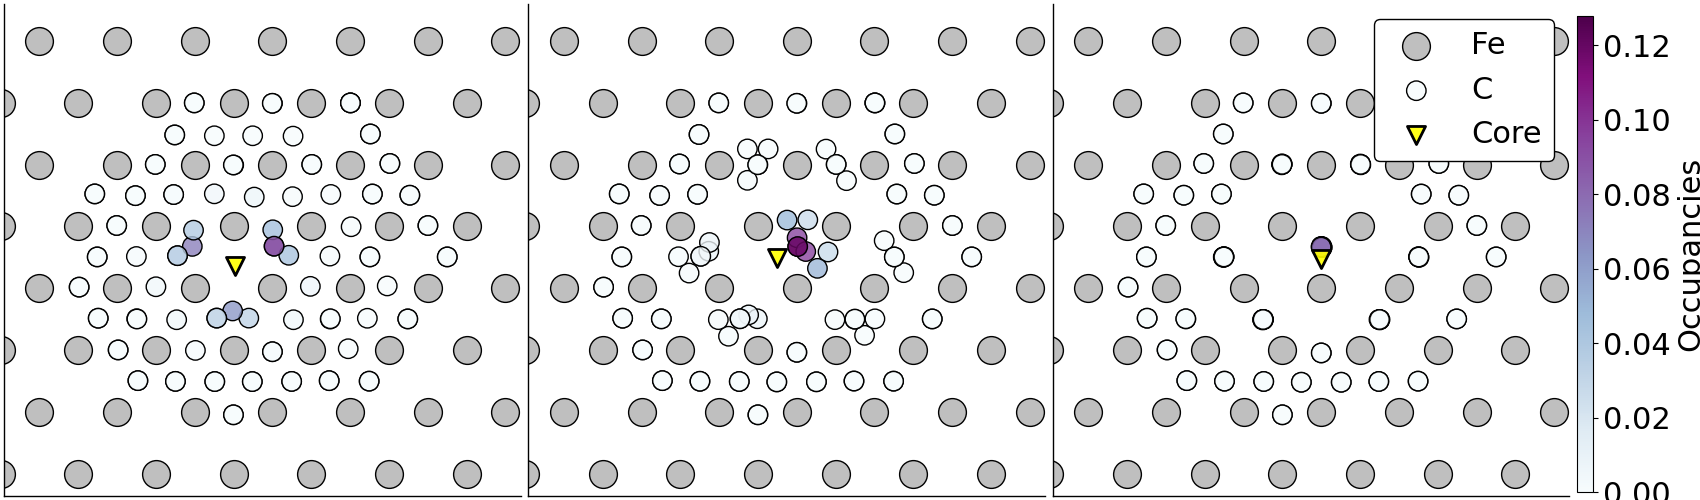
\includegraphics[width=1.\textwidth]{iron/Images/mclean_position_movement_occupancy_forward_alternate.png}
\caption{Positions of trap sites around dislocation segments upon kink-pair formation at a nominal carbon concentration of 30 appm. Path only shown to the hard core to demonstrate smooth mapping of trap sites going from easy to hard core. Equilibrium occupancies shown by coloured circles. \label{fig:kpoccupancies}}
\end{figure}


\end{appendices}

% *************************************** Index ********************************
\printthesisindex % If index is present
\end{document}